\documentclass[10pt,fleqn]{article} % Default font size and left-justified equations
\usepackage[%
    pdftitle={CIN : Cinématique du solide},
    pdfauthor={Xavier Pessoles}]{hyperref}
%\usepackage{pdfpages}

%----------------------------------------------------------------------------------------
%	VARIOUS REQUIRED PACKAGES AND CONFIGURATIONS
%----------------------------------------------------------------------------------------

\usepackage[top=2cm,bottom=2cm,left=2cm,right=2cm,a4paper]{geometry} % Page margins

\usepackage{graphicx} % Required for including pictures
\usepackage{float}
\usepackage[francais]{babel} % English language/hyphenation
\frenchbsetup{StandardLists=true} % Pour éviter la collision babel enumitem pour les listes

\usepackage{enumitem} % Customize lists
\setlist{nolistsep} % Reduce spacing between bullet points and numbered lists

\usepackage{booktabs} % Required for nicer horizontal rules in tables

\usepackage[svgnames]{xcolor} % Required for specifying colors by name
%\definecolor{ocre}{RGB}{243,102,25} % Define the orange color used for highlighting throughout the book
\definecolor{bleuxp}{RGB}{49,133,156} % Couleur ''bleue''
\definecolor{violetf}{RGB}{112,48,160} % Couleur ''violet''

\usepackage{enumitem}
\usepackage{pifont} % Pour les dinglist
\usepackage{multicol}
\usepackage{array} % Centrage vertical dans les tableaux
\usepackage{schemabloc}

% Requis par UPSTI pedagogique
\usepackage{etoolbox}         % Scripting
\usepackage{ifthen}           % Scripting
\usepackage{xargs}            % Pour arguments optionnels multiples
\usepackage{tabularx}         % Tableaux avancés


\usepackage{tikz} % Required for drawing custom shapes

% Définition des booleéns
\newif\iffiche
\newif\ifprof
\newif\iftd
\newif\ifcours
\newif\ifnormal
\newif\ifdifficile
\newif\iftdifficile
\newif\ifcolle
\newif\iflivret
\newif\ifcorrection % True si le corrigé existe, False Sinon

%----------------------------------------------------------------------------------------
%	FONTS
%----------------------------------------------------------------------------------------
\usepackage{bm}
\usepackage{siunitx}
\sisetup{output-decimal-marker = {,}}
\usepackage{textcomp}


\usepackage{avant} % Use the Avantgarde font for headings
%\usepackage{times} % Use the Times font for headings
%\usepackage{mathptmx} % Use the Adobe Times Roman as the default text font together with math symbols from the Sym­bol, Chancery and Com­puter Modern fonts
\usepackage[adobe-utopia]{mathdesign}
\usepackage{microtype} % Slightly tweak font spacing for aesthetics

%% Pour PdfLaTex
\usepackage[utf8]{inputenc} % Required for including letters with accents
\usepackage[T1]{fontenc} % Use 8-bit encoding that has 256 glyphs
% Pour xelatex
%\usepackage{fontspec}

\usepackage{amsmath}
%----------------------------------------------------------------------------------------
%	BIBLIOGRAPHY AND INDEX
%----------------------------------------------------------------------------------------

%\usepackage[style=alphabetic,citestyle=numeric,sorting=nyt,sortcites=true,autopunct=true,babel=hyphen,hyperref=true,abbreviate=false,backref=true,backend=biber]{biblatex}
\usepackage[style=alphabetic,citestyle=numeric,sorting=nyt,sortcites=true,autopunct=true,hyperref=true,abbreviate=false,backref=true,backend=biber]{biblatex}
\addbibresource{bibliography.bib} % BibTeX bibliography file
\defbibheading{bibempty}{}
\usepackage{calc} % For simpler calculation - used for spacing the index letter headings correctly
\usepackage{makeidx} % Required to make an index
\makeindex % Tells LaTeX to create the files required for indexing

%----------------------------------------------------------------------------------------
%	MAIN TABLE OF CONTENTS
%----------------------------------------------------------------------------------------

\usepackage{titletoc} % Required for manipulating the table of contents
\setcounter{tocdepth}{2}     % Dans la table des matieres
\setcounter{secnumdepth}{2}
\contentsmargin{0cm} % Removes the default margin


%----------------------------------------------------------------------------------------
%	PAGE HEADERS
%----------------------------------------------------------------------------------------

\usepackage{fancyhdr} % Required for header and footer configuration

%----------------------------------------------------------------------------------------
%	HYPERLINKS IN THE DOCUMENTS
%----------------------------------------------------------------------------------------


\hypersetup{hidelinks,backref=true,pagebackref=true,hyperindex=true,colorlinks=false,breaklinks=true,urlcolor= ocre,bookmarks=true,bookmarksopen=false,pdftitle={Title},pdfauthor={Author}}
\usepackage{bookmark}
\bookmarksetup{open,numbered,addtohook={%
\ifnum
	\bookmarkget{level}=0 % chapter
	\bookmarksetup{bold}%
\fi
\ifnum
	\bookmarkget{level}=-1 % part
	\bookmarksetup{color=bleuxp,bold}%
\fi}}

%----------------------------------------------------------------------------------------
%	THEOREM STYLES
%----------------------------------------------------------------------------------------

% Conflit avec la police adobe
%\usepackage{amsmath,amsfonts,amssymb,amsthm} % For math equations, theorems, symbols, etc
\usepackage{amsmath,amsthm}

\newcommand{\intoo}[2]{\mathopen{]}#1\,;#2\mathclose{[}}
\newcommand{\ud}{\mathop{\mathrm{{}d}}\mathopen{}}
\newcommand{\intff}[2]{\mathopen{[}#1\,;#2\mathclose{]}}
%\newtheorem{notation}{Notation}[chapter]
\newtheorem{notation}{Notation}[section]

% Boxed/framed environments
\newtheoremstyle{ocrenumbox}% % Theorem style name
{0pt}% Space above
{0pt}% Space below
{\normalfont}% % Body font
{}% Indent amount
{\small\bf\sffamily\color{bleuxp}}% % Theorem head font
{\;}% Punctuation after theorem head
{0.25em}% Space after theorem head
{\small\sffamily\color{bleuxp}\thmname{#1}\nobreakspace\thmnumber%{\@ifnotempty{#1}{}\@upn{#2}}% Theorem text (e.g. Theorem 2.1)
\thmnote{\nobreakspace\the\thm@notefont\sffamily\bfseries\color{black}---\nobreakspace#3.}} % Optional theorem note
\renewcommand{\qedsymbol}{$\blacksquare$}% Optional qed square


% Boite pour les corriges
\newtheoremstyle{correctionbox}% % Theorem style name
{0pt}% Space above
{0pt}% Space below
{\normalfont}% % Body font
{}% Indent amount
{\small\bf\sffamily\color{violet}}% % Theorem head font
{\;}% Punctuation after theorem head
{0.25em}% Space after theorem head
{\small\sffamily\color{bleuxp}\thmname{#1}\nobreakspace\thmnumber%{\@ifnotempty{#1}{}\@upn{#2}}% Theorem text (e.g. Theorem 2.1)
\thmnote{\nobreakspace\the\thm@notefont\sffamily\bfseries\color{black}---\nobreakspace#3.}} % Optional theorem note
\renewcommand{\qedsymbol}{$\blacksquare$}% Optional qed square



\newtheoremstyle{blacknumex}% Theorem style name
{5pt}% Space above
{5pt}% Space below
{\normalfont}% Body font
{} % Indent amount
{\small\bf\sffamily}% Theorem head font
{\;}% Punctuation after theorem head
{0.25em}% Space after theorem head
{\small\sffamily{\tiny\ensuremath{\blacksquare}}\nobreakspace\thmname{#1}\nobreakspace\thmnumber%{\@ifnotempty{#1}{}\@upn{#2}}% Theorem text (e.g. Theorem 2.1)
\thmnote{\nobreakspace\the\thm@notefont\sffamily\bfseries---\nobreakspace#3.}}% Optional theorem note

\newtheoremstyle{blacknumbox} % Theorem style name
{0pt}% Space above
{0pt}% Space below
{\normalfont}% Body font
{}% Indent amount
{\small\bf\sffamily}% Theorem head font
{\;}% Punctuation after theorem head
{0.25em}% Space after theorem head
{\small\sffamily\thmname{#1}\nobreakspace 
\thmnote{\nobreakspace\the\thm@notefont\sffamily\bfseries---\nobreakspace#3.}}% Optional theorem note

% Non-boxed/non-framed environments
\newtheoremstyle{ocrenum}% % Theorem style name
{5pt}% Space above
{5pt}% Space below
{\normalfont}% % Body font
{}% Indent amount
{\small\bf\sffamily\color{bleuxp}}% % Theorem head font
{\;}% Punctuation after theorem head
{0.25em}% Space after theorem head
{\small\sffamily\color{bleuxp}\thmname{#1}\nobreakspace%\thmnumber{\@ifnotempty{#1}{}\@upn{#2}}% Theorem text (e.g. Theorem 2.1)
\thmnote{\nobreakspace\the\thm@notefont\sffamily\bfseries\color{black}---\nobreakspace#3.}} % Optional theorem note
\renewcommand{\qedsymbol}{$\blacksquare$}% Optional qed square
\makeatother

% Environnement pour les titres de parties
\newtheoremstyle{partiebox} 
{0pt}% Space above
{0pt}% Space below
{\normalfont}% Body font
{}% Indent amount
{\small\bf\sffamily}% Theorem head font
{\;}% Punctuation after theorem head
{0.25em}% Space after theorem head




% Defines the theorem text style for each type of theorem to one of the three styles above
\newcounter{dummy} 
\numberwithin{dummy}{section}
\theoremstyle{ocrenumbox}
%\newtheorem{theoremeT}[dummy]{Théorème}
\newtheorem{theoremeT}[dummy]{Théorème}
\newtheorem{resultatT}[dummy]{Résultat}
\newtheorem{savoirT}[dummy]{Savoir}
\newtheorem{methodeT}[dummy]{Méthode}
\newtheorem{objectifT}[dummy]{Objectif}
%\newtheorem{problem}{Problem}[chapter]
\newtheorem{problem}{Problem}[section]
%\newtheorem{exerciseT}{Exercise}[chapter]
\newtheorem{exerciseT}{Exercice}[section]

\theoremstyle{blacknumex}
%\newtheorem{exampleT}{Example}[chapter]
\newtheorem{exempleT}{Exemple}[section]
\newtheorem{termT}{Terminal\\}[section]
\newtheorem{pyT}{Python\\}[section]
\newtheorem{sciT}{Scilab\\}[section]
\newtheorem{pseudoT}{Pseudo Code\\}[section]
\newtheorem{sqlT}{SQL\\}[section]

\theoremstyle{blacknumbox}
%\newtheorem{vocabulary}{Vocabulary}[chapter]
\newtheorem{vocabulary}{Vocabulaire}[section]
%\newtheorem{definitionT}{Definition}[section]
\newtheorem{definitionT}{Définition}[section]
\newtheorem{propT}{Propriété}[section]
\newtheorem{rappelT}{Rappel}[section]
\newtheorem{demoT}{Démonstration}[section]
\newtheorem{corollaryT}[dummy]{Corollaire}
\newtheorem{hypoT}{Hypothèse(s)}

\theoremstyle{ocrenum}
\newtheorem{proposition}[dummy]{Proposition}

\theoremstyle{partiebox}
\newtheorem{titrepartieT}[]{}
\newtheorem{titrechapitreT}[]{}

\theoremstyle{correctionbox}
\newtheorem{correctionT}[dummy]{\color{violet}{Correction}}

%----------------------------------------------------------------------------------------
%	DEFINITION OF COLORED BOXES
%----------------------------------------------------------------------------------------

\RequirePackage[framemethod=tikz]{mdframed} % Required for creating the theorem, definition, exercise and corollary boxes

% Theorem box
\newmdenv[skipabove=7pt,
skipbelow=7pt,
backgroundcolor=bleuxp!10,
linecolor=bleuxp,
innerleftmargin=5pt,
innerrightmargin=5pt,
innertopmargin=5pt,
leftmargin=0cm,
rightmargin=0cm,
innerbottommargin=5pt]{tBox}


% Correction
\newmdenv[skipabove=7pt,
skipbelow=7pt,
backgroundcolor=violet!10,
linecolor=violet,
innerleftmargin=5pt,
innerrightmargin=5pt,
innertopmargin=5pt,
leftmargin=0cm,
rightmargin=0cm,
innerbottommargin=5pt]{coBox}


% Exercise box	  
\newmdenv[skipabove=7pt,
skipbelow=7pt,
rightline=false,
leftline=true,
topline=false,
bottomline=false,
backgroundcolor=bleuxp!10,
linecolor=bleuxp,
innerleftmargin=5pt,
innerrightmargin=5pt,
innertopmargin=5pt,
innerbottommargin=5pt,
leftmargin=0cm,
rightmargin=0cm,
linewidth=4pt]{eBox}	

% Definition box
\newmdenv[skipabove=7pt,
skipbelow=7pt,
rightline=false,
leftline=true,
topline=false,
bottomline=false,
backgroundcolor=bleuxp!10,
linecolor=bleuxp,
innerleftmargin=5pt,
innerrightmargin=5pt,
innertopmargin=0pt,
leftmargin=0cm,
rightmargin=0cm,
linewidth=4pt,
innerbottommargin=0pt]{dBox}	

% Demonstration box
\newmdenv[skipabove=7pt,
skipbelow=7pt,
rightline=false,
leftline=true,
topline=false,
bottomline=false,
%backgroundcolor=bleuxp!10,
linecolor=bleuxp,
innerleftmargin=5pt,
innerrightmargin=5pt,
innertopmargin=0pt,
leftmargin=0cm,
rightmargin=0cm,
linewidth=4pt,
innerbottommargin=0pt]{demoBox}	

% Corollary box
\newmdenv[skipabove=7pt,
skipbelow=7pt,
rightline=false,
leftline=true,
topline=false,
bottomline=false,
linecolor=gray,
backgroundcolor=black!5,
innerleftmargin=5pt,
innerrightmargin=5pt,
innertopmargin=5pt,
leftmargin=0cm,
rightmargin=0cm,
linewidth=4pt,
innerbottommargin=5pt]{cBox}


% Hypothèses
\newmdenv[skipabove=7pt,
skipbelow=7pt,
rightline=false,
leftline=true,
topline=false,
bottomline=false,
linecolor=gray,
backgroundcolor=black!5,
innerleftmargin=5pt,
innerrightmargin=5pt,
innertopmargin=5pt,
leftmargin=0cm,
rightmargin=0cm,
linewidth=4pt,
innerbottommargin=5pt]{hyBox}


% Boite pour le titre de la partie (pBox)
\newmdenv[skipabove=7pt,
skipbelow=7pt,
rightline=true,
leftline=false,
topline=false,
bottomline=false,
linecolor=bleuxp,
backgroundcolor=none,
innerleftmargin=5pt,
innerrightmargin=5pt,
innertopmargin=5pt,
leftmargin=0cm,
rightmargin=0cm,
linewidth=4pt,
innerbottommargin=5pt]{pBox}

% Boite pour le titre du chapitre (chBox)
\newmdenv[skipabove=7pt,
skipbelow=7pt,
rightline=false,
leftline=true,
topline=false,
bottomline=false,
linecolor=bleuxp,
%backgroundcolor=black!5,
innerleftmargin=5pt,
innerrightmargin=5pt,
innertopmargin=5pt,
leftmargin=0cm,
rightmargin=0cm,
linewidth=4pt,
innerbottommargin=5pt]{chBox}


% Boite pour les exemples
\newmdenv[skipabove=7pt,
skipbelow=7pt,
rightline=false,
leftline=true,
topline=false,
bottomline=false,
linecolor=gray,
backgroundcolor=white,
innerleftmargin=5pt,
innerrightmargin=5pt,
innertopmargin=5pt,
leftmargin=0cm,
rightmargin=0cm,
linewidth=4pt,
innerbottommargin=5pt]{exBox}

% Boite pour le terminal
\newmdenv[skipabove=7pt,
skipbelow=7pt,
rightline=false,
leftline=true,
topline=false,
bottomline=false,
linecolor=gray,
backgroundcolor=white,
innerleftmargin=5pt,
innerrightmargin=5pt,
innertopmargin=5pt,
leftmargin=0cm,
rightmargin=0cm,
linewidth=4pt,
innerbottommargin=5pt]{termBox}


% Boite pour Python
\newmdenv[skipabove=7pt,
skipbelow=7pt,
rightline=false,
leftline=true,
topline=false,
bottomline=false,
linecolor=gray,
backgroundcolor=white,
innerleftmargin=5pt,
innerrightmargin=5pt,
innertopmargin=0pt,
leftmargin=0cm,
rightmargin=0cm,
linewidth=4pt,
innerbottommargin=5pt]{pyBox}

% Boite pour scilab
\newmdenv[skipabove=7pt,
skipbelow=7pt,
rightline=false,
leftline=true,
topline=false,
bottomline=false,
linecolor=gray,
backgroundcolor=white,
innerleftmargin=5pt,
innerrightmargin=5pt,
innertopmargin=5pt,
leftmargin=0cm,
rightmargin=0cm,
linewidth=4pt,
innerbottommargin=5pt]{sciBox}


% Boite pour pseudo
\newmdenv[skipabove=7pt,
skipbelow=7pt,
rightline=false,
leftline=true,
topline=false,
bottomline=false,
linecolor=gray,
backgroundcolor=white,
innerleftmargin=5pt,
innerrightmargin=5pt,
innertopmargin=5pt,
leftmargin=0cm,
rightmargin=0cm,
linewidth=4pt,
innerbottommargin=5pt]{pseudoBox}

% Boite pour pseudo
\newmdenv[skipabove=7pt,
skipbelow=7pt,
rightline=false,
leftline=true,
topline=false,
bottomline=false,
linecolor=gray,
backgroundcolor=white,
innerleftmargin=5pt,
innerrightmargin=5pt,
innertopmargin=5pt,
leftmargin=0cm,
rightmargin=0cm,
linewidth=4pt,
innerbottommargin=5pt]{sqlBox}


% Creates an environment for each type of theorem and assigns it a theorem text style from the "Theorem Styles" section above and a colored box from above
\newenvironment{theorem}{\begin{tBox}\begin{theoremeT}}{\end{theoremeT}\end{tBox}}
\newenvironment{resultat}{\begin{tBox}\begin{resultatT}}{\end{resultatT}\end{tBox}}
\newenvironment{methode}{\begin{tBox}\begin{methodeT}}{\end{methodeT}\end{tBox}}
\newenvironment{savoir}{\begin{tBox}\begin{savoirT}}{\end{savoirT}\end{tBox}}
\newenvironment{obj}{\begin{tBox}\begin{objectifT}}{\end{objectifT}\end{tBox}}
\newenvironment{corrige}{\begin{coBox}\begin{correctionT}}{\end{correctionT}\end{coBox}}
\newenvironment{exercise}{\begin{eBox}\begin{exerciseT}}{\hfill{\color{bleuxp}\tiny\ensuremath{\blacksquare}}\end{exerciseT}\end{eBox}}				  
\newenvironment{exercice}{\begin{eBox}\begin{exerciseT}}{\hfill{\color{bleuxp}\tiny\ensuremath{\blacksquare}}\end{exerciseT}\end{eBox}}				  

\newenvironment{definition}{\begin{dBox}\begin{definitionT}}{\end{definitionT}\end{dBox}}
\newenvironment{prop}{\begin{dBox}\begin{propT}}{\end{propT}\end{dBox}}	
\newenvironment{rappel}{\begin{dBox}\begin{rappelT}}{\end{rappelT}\end{dBox}}	
\newenvironment{defi}{\begin{dBox}\begin{definitionT}}{\end{definitionT}\end{dBox}}	
\newenvironment{demo}{\begin{demoBox}\begin{demoT}}{\end{demoT}\end{demoBox}}	
%\newenvironment{exemple}{\begin{exempleT}}{\hfill{\tiny\ensuremath{\blacksquare}}\end{exempleT}}		
\newenvironment{corollary}{\begin{cBox}\begin{corollaryT}}{\end{corollaryT}\end{cBox}}
\newenvironment{hypo}{\begin{hyBox}\begin{hypoT}}{\end{hypoT}\end{hyBox}}	\newenvironment{exemple}{\begin{exBox}\begin{exempleT}}{\hfill{\tiny\ensuremath{\blacksquare}}\end{exempleT}\end{exBox}}	
\newenvironment{titrepartie}{\begin{pBox}\begin{titrepartieT}}{\end{titrepartieT}\end{pBox}}	
\newenvironment{titrechapitre}{\begin{chBox}\begin{titrechapitreT}}{\end{titrechapitreT}\end{chBox}}	

\newenvironment{term}{ \begin{termBox}\begin{termT}}{\end{termT}\end{termBox}}
\newenvironment{py}{ \begin{pyBox}\begin{pyT}}{\end{pyT}\end{pyBox}}
\newenvironment{sci}{ \begin{sciBox}\begin{sciT}}{\end{sciT}\end{sciBox}}
\newenvironment{pseudo}{ \begin{pseudoBox}\begin{pseudoT}}{\end{pseudoT}\end{pseudoBox}}
\newenvironment{envsql}{ \begin{sqlBox}\begin{sqlT}}{\end{sqlT}\end{sqlBox}}


%----------------------------------------------------------------------------------------
%	REMARK ENVIRONMENT
%----------------------------------------------------------------------------------------

\newenvironment{remark}{\par\vspace{10pt}\small % Vertical white space above the remark and smaller font size
\begin{list}{}{
\leftmargin=35pt % Indentation on the left
\rightmargin=25pt}\item\ignorespaces % Indentation on the right
\makebox[-2.5pt]{\begin{tikzpicture}[overlay]
\node[draw=bleuxp!60,line width=1pt,circle,fill=bleuxp!25,font=\sffamily\bfseries,inner sep=2pt,outer sep=0pt] at (-15pt,0pt){\textcolor{bleuxp}{R}};\end{tikzpicture}} % Orange R in a circle
\advance\baselineskip -1pt}{\end{list}\vskip5pt} % Tighter line spacing and white space after remark

\newenvironment{rem}{\par\vspace{10pt}\small % Vertical white space above the remark and smaller font size
\begin{list}{}{
\leftmargin=35pt % Indentation on the left
\rightmargin=25pt}\item\ignorespaces % Indentation on the right
\makebox[-2.5pt]{\begin{tikzpicture}[overlay]
\node[draw=bleuxp!60,line width=1pt,circle,fill=bleuxp!25,font=\sffamily\bfseries,inner sep=2pt,outer sep=0pt] at (-15pt,0pt){\textcolor{bleuxp}{R}};\end{tikzpicture}} % Orange R in a circle
\advance\baselineskip -1pt}{\end{list}\vskip5pt} % Tighter line spacing and white space after remark


\newenvironment{warn}{\par\vspace{10pt}\small % Vertical white space above the remark and smaller font size
\begin{list}{}{
\leftmargin=35pt % Indentation on the left
\rightmargin=25pt}\item\ignorespaces % Indentation on the right
\makebox[-2.5pt]{\begin{tikzpicture}[overlay]
\node[draw=red!60,line width=1pt,circle,fill=red!25,font=\sffamily\bfseries,inner sep=2pt,outer sep=0pt] at (-15pt,0pt){\textcolor{black}{!}};\end{tikzpicture}} % Point d'exclamation dans un cercle
\advance\baselineskip -1pt}{\end{list}\vskip5pt} % Tighter line spacing and white space after remark


%%%%%%%%%%%%%%%%%%%%%%%%%%%%%%%%%%%%%%%%%
% Original author:
% Mathias Legrand (legrand.mathias@gmail.com) with modifications by:
% Vel (vel@latextemplates.com)
% License:
% CC BY-NC-SA 3.0 (http://creativecommons.org/licenses/by-nc-sa/3.0/)
%%%%%%%%%%%%%%%%%%%%%%%%%%%%%%%%%%%%%%%%%

%----------------------------------------------------------------------------------------
%	VARIOUS REQUIRED PACKAGES AND CONFIGURATIONS
%----------------------------------------------------------------------------------------

% Définition des booleéns
\newif\iffiche
\newif\ifprof
\newif\iftd
\newif\ifcours


\usepackage[top=2.5cm,bottom=2cm,left=2cm,right=2cm,headsep=40pt,a4paper]{geometry} % Page margins

\usepackage{graphicx} % Required for including pictures
\graphicspath{{images/}} % Specifies the directory where pictures are stored

\usepackage{lipsum} % Inserts dummy text

\usepackage{tikz} % Required for drawing custom shapes

\usepackage[french]{babel} % English language/hyphenation
\frenchbsetup{StandardLists=true} % Pour éviter la collision babel enumitem pour les listes

\usepackage{enumitem} % Customize lists
\setlist{nolistsep} % Reduce spacing between bullet points and numbered lists

\usepackage{booktabs} % Required for nicer horizontal rules in tables

\usepackage{colortbl} % Couleur dans les tableaux

\usepackage{xcolor} % Required for specifying colors by name
%\definecolor{ocre}{RGB}{243,102,25} % Define the orange color used for highlighting throughout the book
\definecolor{ocre}{RGB}{49,133,156} % Couleur ''bleue''
\definecolor{violetf}{RGB}{112,48,160} % Couleur ''violet''
\usepackage{enumitem}
\usepackage{pifont} % Pour les dinglist
\usepackage{multicol}
\usepackage{array} % Centrage vertical dans les tableaux

%----------------------------------------------------------------------------------------
%	FONTS
%----------------------------------------------------------------------------------------

\usepackage{avant} % Use the Avantgarde font for headings
%\usepackage{times} % Use the Times font for headings
%\usepackage{mathptmx} % Use the Adobe Times Roman as the default text font together with math symbols from the Sym­bol, Chancery and Com­puter Modern fonts
\usepackage[adobe-utopia]{mathdesign}
\usepackage{microtype} % Slightly tweak font spacing for aesthetics
\usepackage[utf8]{inputenc} % Required for including letters with accents
\usepackage[T1]{fontenc} % Use 8-bit encoding that has 256 glyphs

%----------------------------------------------------------------------------------------
%	BIBLIOGRAPHY AND INDEX
%----------------------------------------------------------------------------------------

\usepackage[style=alphabetic,citestyle=numeric,sorting=nyt,sortcites=true,autopunct=true,babel=hyphen,hyperref=true,abbreviate=false,backref=true,backend=biber]{biblatex}
\addbibresource{bibliography.bib} % BibTeX bibliography file
\defbibheading{bibempty}{}

\usepackage{calc} % For simpler calculation - used for spacing the index letter headings correctly
\usepackage{makeidx} % Required to make an index
\makeindex % Tells LaTeX to create the files required for indexing

%----------------------------------------------------------------------------------------
%	MAIN TABLE OF CONTENTS
%----------------------------------------------------------------------------------------

\usepackage{titletoc} % Required for manipulating the table of contents

\setcounter{tocdepth}{2}     % Dans la table des matieres
\setcounter{secnumdepth}{2}

\contentsmargin{0cm} % Removes the default margin

% Part text styling
\titlecontents{part}[0cm]
{\addvspace{20pt}\centering\large\bfseries}
{}
{}
{}

% Chapter text styling
\titlecontents{chapter}[1.25cm] % Indentation
{\addvspace{12pt}\large\sffamily\bfseries} % Spacing and font options for chapters
{\color{ocre!60}\contentslabel[\Large\thecontentslabel]{1.25cm}\color{ocre}} % Chapter number
{\color{ocre}}  
{\color{ocre!60}\normalsize\;\titlerule*[.5pc]{.}\;\thecontentspage} % Page number

% Section text styling
\titlecontents{section}[1.25cm] % Indentation
{\addvspace{3pt}\sffamily\bfseries} % Spacing and font options for sections
{\color{ocre!60}\contentslabel[\thecontentslabel]{1.25cm} \color{ocre}} % Section number
{\color{ocre}}
{\hfill\color{ocre!60}\thecontentspage} % Page number
[]

% Subsection text styling
\titlecontents{subsection}[1.25cm] % Indentation
{\addvspace{1pt}\sffamily\small} % Spacing and font options for subsections
{\contentslabel[\thecontentslabel]{1.25cm}} % Subsection number
{}
{\ \titlerule*[.5pc]{.}\;\thecontentspage} % Page number
[]


% Subsection text styling
\titlecontents{subsubsection}[1.25cm] % Indentation
{\addvspace{1pt}\sffamily\small} % Spacing and font options for subsections
{\contentslabel[\thecontentslabel]{1.25cm}} % Subsection number
{}
{\ \titlerule*[.5pc]{.}\;\thecontentspage} % Page number
[]

% List of figures
\titlecontents{figure}[0em]
{\addvspace{-5pt}\sffamily}
{\thecontentslabel\hspace*{1em}}
{}
{\ \titlerule*[.5pc]{.}\;\thecontentspage}
[]

% List of tables
\titlecontents{table}[0em]
{\addvspace{-5pt}\sffamily}
{\thecontentslabel\hspace*{1em}}
{}
{\ \titlerule*[.5pc]{.}\;\thecontentspage}
[]

%----------------------------------------------------------------------------------------
%	MINI TABLE OF CONTENTS IN PART HEADS
%----------------------------------------------------------------------------------------

% Chapter text styling
\titlecontents{lchapter}[0em] % Indenting
{\addvspace{15pt}\large\sffamily\bfseries} % Spacing and font options for chapters
{\color{ocre}\contentslabel[\Large\thecontentslabel]{1.25cm}\color{ocre}} % Chapter number
{}  
{\color{ocre}\normalsize\sffamily\bfseries\;\titlerule*[.5pc]{.}\;\thecontentspage} % Page number

% Section text styling
\titlecontents{lsection}[0em] % Indenting
{\sffamily\small} % Spacing and font options for sections
{\contentslabel[\thecontentslabel]{1.25cm}} % Section number
{}
{}

% Subsection text styling
\titlecontents{lsubsection}[.5em] % Indentation
{\normalfont\footnotesize\sffamily} % Font settings
{}
{}
{}

%----------------------------------------------------------------------------------------
%	PAGE HEADERS
%----------------------------------------------------------------------------------------

\usepackage{fancyhdr} % Required for header and footer configuration



\pagestyle{fancy}
 \renewcommand{\headrulewidth}{0pt}
 \fancyhead{}
 \fancyhead[L]{%
 \noindent\begin{minipage}[c]{2.6cm}%
 
\includegraphics[width=2cm]{png/logo_lycee.png}%
 \end{minipage}}

\fancyhead[C]{\rule{8cm}{.5pt}}

 \fancyhead[R]{%
 \noindent\begin{minipage}[c]{3cm}
 \begin{flushright}
 \footnotesize{\textit{\textsf{\xxtete}}}%
 \end{flushright}
 \end{minipage}
}


\fancyfoot[C]{\rule{12cm}{.5pt}}
\renewcommand{\footrulewidth}{0.2pt}
\fancyfoot[C]{\footnotesize{\bfseries \thepage}}
\fancyfoot[L]{ 
\begin{minipage}[c]{.2\linewidth}
\noindent\footnotesize{{\xxauteur}}
\end{minipage}}


\fancyfoot[R]{\footnotesize{\xxpied}
\ifthenelse{\isodd{\value{page}}}{
\begin{tikzpicture}[overlay]
\node[shape=rectangle, 
      rounded corners = .25 cm,
	  draw= ocre,
	  line width=2pt, 
	  fill = ocre!10,
	  minimum width  = 2.5cm,
	  minimum height = 3cm,] at (\xxposongletx,\xxposonglety) {};
\node at (\xxposonglettext,\xxposonglety) {\rotatebox{90}{\textbf{\large\color{ocre}{\xxonglet}}}};
%{};
\end{tikzpicture}}{}
}
%
%
%
% Removes the header from odd empty pages at the end of chapters
\makeatletter
\renewcommand{\cleardoublepage}{
\clearpage\ifodd\c@page\else
\hbox{}
\vspace*{\fill}
\thispagestyle{empty}
\newpage
\fi}

\fancypagestyle{plain}{%
\fancyhf{} % vide l’en-tête et le pied~de~page.
%\fancyfoot[C]{\bfseries \thepage} % numéro de la page en cours en gras
% et centré en pied~de~page.
\fancyfoot[R]{\footnotesize{\xxpied}}
\fancyfoot[C]{\rule{12cm}{.5pt}}
\renewcommand{\footrulewidth}{0.2pt}
\fancyfoot[C]{\footnotesize{\bfseries \thepage}}
\fancyfoot[L]{ 
\begin{minipage}[c]{.2\linewidth}
\noindent\footnotesize{{\xxauteur}}
\end{minipage}}}



%----------------------------------------------------------------------------------------
%	THEOREM STYLES
%----------------------------------------------------------------------------------------

% Conflit avec la police adobe
%\usepackage{amsmath,amsfonts,amssymb,amsthm} % For math equations, theorems, symbols, etc
\usepackage{amsmath,amsthm}

\newcommand{\intoo}[2]{\mathopen{]}#1\,;#2\mathclose{[}}
\newcommand{\ud}{\mathop{\mathrm{{}d}}\mathopen{}}
\newcommand{\intff}[2]{\mathopen{[}#1\,;#2\mathclose{]}}
%\newtheorem{notation}{Notation}[chapter]
\newtheorem{notation}{Notation}[section]

% Boxed/framed environments
\newtheoremstyle{ocrenumbox}% % Theorem style name
{0pt}% Space above
{0pt}% Space below
{\normalfont}% % Body font
{}% Indent amount
{\small\bf\sffamily\color{ocre}}% % Theorem head font
{\;}% Punctuation after theorem head
{0.25em}% Space after theorem head
{\small\sffamily\color{ocre}\thmname{#1}\nobreakspace\thmnumber%{\@ifnotempty{#1}{}\@upn{#2}}% Theorem text (e.g. Theorem 2.1)
\thmnote{\nobreakspace\the\thm@notefont\sffamily\bfseries\color{black}---\nobreakspace#3.}} % Optional theorem note
\renewcommand{\qedsymbol}{$\blacksquare$}% Optional qed square


% Boite pour les corriges
\newtheoremstyle{correctionbox}% % Theorem style name
{0pt}% Space above
{0pt}% Space below
{\normalfont}% % Body font
{}% Indent amount
{\small\bf\sffamily\color{violet}}% % Theorem head font
{\;}% Punctuation after theorem head
{0.25em}% Space after theorem head
{\small\sffamily\color{ocre}\thmname{#1}\nobreakspace\thmnumber%{\@ifnotempty{#1}{}\@upn{#2}}% Theorem text (e.g. Theorem 2.1)
\thmnote{\nobreakspace\the\thm@notefont\sffamily\bfseries\color{black}---\nobreakspace#3.}} % Optional theorem note
\renewcommand{\qedsymbol}{$\blacksquare$}% Optional qed square



\newtheoremstyle{blacknumex}% Theorem style name
{5pt}% Space above
{5pt}% Space below
{\normalfont}% Body font
{} % Indent amount
{\small\bf\sffamily}% Theorem head font
{\;}% Punctuation after theorem head
{0.25em}% Space after theorem head
{\small\sffamily{\tiny\ensuremath{\blacksquare}}\nobreakspace\thmname{#1}\nobreakspace\thmnumber%{\@ifnotempty{#1}{}\@upn{#2}}% Theorem text (e.g. Theorem 2.1)
\thmnote{\nobreakspace\the\thm@notefont\sffamily\bfseries---\nobreakspace#3.}}% Optional theorem note

\newtheoremstyle{blacknumbox} % Theorem style name
{0pt}% Space above
{0pt}% Space below
{\normalfont}% Body font
{}% Indent amount
{\small\bf\sffamily}% Theorem head font
{\;}% Punctuation after theorem head
{0.25em}% Space after theorem head
{\small\sffamily\thmname{#1}\nobreakspace 
\thmnote{\nobreakspace\the\thm@notefont\sffamily\bfseries---\nobreakspace#3.}}% Optional theorem note

% Non-boxed/non-framed environments
\newtheoremstyle{ocrenum}% % Theorem style name
{5pt}% Space above
{5pt}% Space below
{\normalfont}% % Body font
{}% Indent amount
{\small\bf\sffamily\color{ocre}}% % Theorem head font
{\;}% Punctuation after theorem head
{0.25em}% Space after theorem head
{\small\sffamily\color{ocre}\thmname{#1}\nobreakspace%\thmnumber{\@ifnotempty{#1}{}\@upn{#2}}% Theorem text (e.g. Theorem 2.1)
\thmnote{\nobreakspace\the\thm@notefont\sffamily\bfseries\color{black}---\nobreakspace#3.}} % Optional theorem note
\renewcommand{\qedsymbol}{$\blacksquare$}% Optional qed square
\makeatother

% Environnement pour les titres de parties
\newtheoremstyle{partiebox} 
{0pt}% Space above
{0pt}% Space below
{\normalfont}% Body font
{}% Indent amount
{\small\bf\sffamily}% Theorem head font
{\;}% Punctuation after theorem head
{0.25em}% Space after theorem head




% Defines the theorem text style for each type of theorem to one of the three styles above
\newcounter{dummy} 
\numberwithin{dummy}{section}
\theoremstyle{ocrenumbox}
%\newtheorem{theoremeT}[dummy]{Théorème}
\newtheorem{theoremeT}[dummy]{Théorème}
\newtheorem{resultatT}[dummy]{Résultat}
\newtheorem{savoirT}[dummy]{Savoir}
\newtheorem{methodeT}[dummy]{Méthode}
\newtheorem{objectifT}[dummy]{Objectif}
%\newtheorem{problem}{Problem}[chapter]
\newtheorem{problem}{Problem}[section]
%\newtheorem{exerciseT}{Exercise}[chapter]
\newtheorem{exerciseT}{Exercice}[section]

\theoremstyle{blacknumex}
%\newtheorem{exampleT}{Example}[chapter]
\newtheorem{exempleT}{Exemple}[section]
\newtheorem{termT}{Terminal\\}[section]
\newtheorem{pyT}{Python\\}[section]
\newtheorem{sciT}{Scilab\\}[section]
\newtheorem{pseudoT}{Pseudo Code\\}[section]
\newtheorem{sqlT}{SQL\\}[section]

\theoremstyle{blacknumbox}
%\newtheorem{vocabulary}{Vocabulary}[chapter]
\newtheorem{vocabulary}{Vocabulaire}[section]
%\newtheorem{definitionT}{Definition}[section]
\newtheorem{definitionT}{Définition}[section]
\newtheorem{demoT}{Démonstration}[section]
\newtheorem{corollaryT}[dummy]{Corollaire}
\newtheorem{hypoT}{Hypothèse(s)}

\theoremstyle{ocrenum}
\newtheorem{proposition}[dummy]{Proposition}

\theoremstyle{partiebox}
\newtheorem{titrepartieT}[]{}
\newtheorem{titrechapitreT}[]{}

\theoremstyle{correctionbox}
\newtheorem{correctionT}[dummy]{\color{violet}{Correction}}

%----------------------------------------------------------------------------------------
%	DEFINITION OF COLORED BOXES
%----------------------------------------------------------------------------------------

\RequirePackage[framemethod=tikz]{mdframed} % Required for creating the theorem, definition, exercise and corollary boxes

% Theorem box
\newmdenv[skipabove=7pt,
skipbelow=7pt,
backgroundcolor=ocre!10,
linecolor=ocre,
innerleftmargin=5pt,
innerrightmargin=5pt,
innertopmargin=5pt,
leftmargin=0cm,
rightmargin=0cm,
innerbottommargin=5pt]{tBox}


% Correction
\newmdenv[skipabove=7pt,
skipbelow=7pt,
backgroundcolor=violet!10,
linecolor=violet,
innerleftmargin=5pt,
innerrightmargin=5pt,
innertopmargin=5pt,
leftmargin=0cm,
rightmargin=0cm,
innerbottommargin=5pt]{coBox}


% Exercise box	  
\newmdenv[skipabove=7pt,
skipbelow=7pt,
rightline=false,
leftline=true,
topline=false,
bottomline=false,
backgroundcolor=ocre!10,
linecolor=ocre,
innerleftmargin=5pt,
innerrightmargin=5pt,
innertopmargin=5pt,
innerbottommargin=5pt,
leftmargin=0cm,
rightmargin=0cm,
linewidth=4pt]{eBox}	

% Definition box
\newmdenv[skipabove=7pt,
skipbelow=7pt,
rightline=false,
leftline=true,
topline=false,
bottomline=false,
backgroundcolor=ocre!10,
linecolor=ocre,
innerleftmargin=5pt,
innerrightmargin=5pt,
innertopmargin=0pt,
leftmargin=0cm,
rightmargin=0cm,
linewidth=4pt,
innerbottommargin=0pt]{dBox}	

% Demonstration box
\newmdenv[skipabove=7pt,
skipbelow=7pt,
rightline=false,
leftline=true,
topline=false,
bottomline=false,
%backgroundcolor=ocre!10,
linecolor=ocre,
innerleftmargin=5pt,
innerrightmargin=5pt,
innertopmargin=0pt,
leftmargin=0cm,
rightmargin=0cm,
linewidth=4pt,
innerbottommargin=0pt]{demoBox}	

% Corollary box
\newmdenv[skipabove=7pt,
skipbelow=7pt,
rightline=false,
leftline=true,
topline=false,
bottomline=false,
linecolor=gray,
backgroundcolor=black!5,
innerleftmargin=5pt,
innerrightmargin=5pt,
innertopmargin=5pt,
leftmargin=0cm,
rightmargin=0cm,
linewidth=4pt,
innerbottommargin=5pt]{cBox}


% Hypothèses
\newmdenv[skipabove=7pt,
skipbelow=7pt,
rightline=false,
leftline=true,
topline=false,
bottomline=false,
linecolor=gray,
backgroundcolor=black!5,
innerleftmargin=5pt,
innerrightmargin=5pt,
innertopmargin=5pt,
leftmargin=0cm,
rightmargin=0cm,
linewidth=4pt,
innerbottommargin=5pt]{hyBox}


% Boite pour le titre de la partie (pBox)
\newmdenv[skipabove=7pt,
skipbelow=7pt,
rightline=true,
leftline=false,
topline=false,
bottomline=false,
linecolor=ocre,
backgroundcolor=none,
innerleftmargin=5pt,
innerrightmargin=5pt,
innertopmargin=5pt,
leftmargin=0cm,
rightmargin=0cm,
linewidth=4pt,
innerbottommargin=5pt]{pBox}

% Boite pour le titre du chapitre (chBox)
\newmdenv[skipabove=7pt,
skipbelow=7pt,
rightline=false,
leftline=true,
topline=false,
bottomline=false,
linecolor=ocre,
%backgroundcolor=black!5,
innerleftmargin=5pt,
innerrightmargin=5pt,
innertopmargin=5pt,
leftmargin=0cm,
rightmargin=0cm,
linewidth=4pt,
innerbottommargin=5pt]{chBox}


% Boite pour les exemples
\newmdenv[skipabove=7pt,
skipbelow=7pt,
rightline=false,
leftline=true,
topline=false,
bottomline=false,
linecolor=gray,
backgroundcolor=white,
innerleftmargin=5pt,
innerrightmargin=5pt,
innertopmargin=5pt,
leftmargin=0cm,
rightmargin=0cm,
linewidth=4pt,
innerbottommargin=5pt]{exBox}

% Boite pour le terminal
\newmdenv[skipabove=7pt,
skipbelow=7pt,
rightline=false,
leftline=true,
topline=false,
bottomline=false,
linecolor=gray,
backgroundcolor=white,
innerleftmargin=5pt,
innerrightmargin=5pt,
innertopmargin=5pt,
leftmargin=0cm,
rightmargin=0cm,
linewidth=4pt,
innerbottommargin=5pt]{termBox}


% Boite pour Python
\newmdenv[skipabove=7pt,
skipbelow=7pt,
rightline=false,
leftline=true,
topline=false,
bottomline=false,
linecolor=gray,
backgroundcolor=white,
innerleftmargin=5pt,
innerrightmargin=5pt,
innertopmargin=5pt,
leftmargin=0cm,
rightmargin=0cm,
linewidth=4pt,
innerbottommargin=5pt]{pyBox}

% Boite pour scilab
\newmdenv[skipabove=7pt,
skipbelow=7pt,
rightline=false,
leftline=true,
topline=false,
bottomline=false,
linecolor=gray,
backgroundcolor=white,
innerleftmargin=5pt,
innerrightmargin=5pt,
innertopmargin=5pt,
leftmargin=0cm,
rightmargin=0cm,
linewidth=4pt,
innerbottommargin=5pt]{sciBox}


% Boite pour pseudo
\newmdenv[skipabove=7pt,
skipbelow=7pt,
rightline=false,
leftline=true,
topline=false,
bottomline=false,
linecolor=gray,
backgroundcolor=white,
innerleftmargin=5pt,
innerrightmargin=5pt,
innertopmargin=5pt,
leftmargin=0cm,
rightmargin=0cm,
linewidth=4pt,
innerbottommargin=5pt]{pseudoBox}

% Boite pour pseudo
\newmdenv[skipabove=7pt,
skipbelow=7pt,
rightline=false,
leftline=true,
topline=false,
bottomline=false,
linecolor=gray,
backgroundcolor=white,
innerleftmargin=5pt,
innerrightmargin=5pt,
innertopmargin=5pt,
leftmargin=0cm,
rightmargin=0cm,
linewidth=4pt,
innerbottommargin=5pt]{sqlBox}


% Creates an environment for each type of theorem and assigns it a theorem text style from the "Theorem Styles" section above and a colored box from above
\newenvironment{theorem}{\begin{tBox}\begin{theoremeT}}{\end{theoremeT}\end{tBox}}
\newenvironment{resultat}{\begin{tBox}\begin{resultatT}}{\end{resultatT}\end{tBox}}
\newenvironment{methode}{\begin{tBox}\begin{methodeT}}{\end{methodeT}\end{tBox}}
\newenvironment{savoir}{\begin{tBox}\begin{savoirT}}{\end{savoirT}\end{tBox}}
\newenvironment{obj}{\begin{tBox}\begin{objectifT}}{\end{objectifT}\end{tBox}}
\newenvironment{corrige}{\begin{coBox}\begin{correctionT}}{\end{correctionT}\end{coBox}}
\newenvironment{exercise}{\begin{eBox}\begin{exerciseT}}{\hfill{\color{ocre}\tiny\ensuremath{\blacksquare}}\end{exerciseT}\end{eBox}}				  
\newenvironment{exercice}{\begin{eBox}\begin{exerciseT}}{\hfill{\color{ocre}\tiny\ensuremath{\blacksquare}}\end{exerciseT}\end{eBox}}				  

\newenvironment{definition}{\begin{dBox}\begin{definitionT}}{\end{definitionT}\end{dBox}}	
\newenvironment{defi}{\begin{dBox}\begin{definitionT}}{\end{definitionT}\end{dBox}}	
\newenvironment{demo}{\begin{demoBox}\begin{demoT}}{\end{demoT}\end{demoBox}}	
%\newenvironment{exemple}{\begin{exempleT}}{\hfill{\tiny\ensuremath{\blacksquare}}\end{exempleT}}		
\newenvironment{corollary}{\begin{cBox}\begin{corollaryT}}{\end{corollaryT}\end{cBox}}
\newenvironment{hypo}{\begin{hyBox}\begin{hypoT}}{\end{hypoT}\end{hyBox}}	\newenvironment{exemple}{\begin{exBox}\begin{exempleT}}{\hfill{\tiny\ensuremath{\blacksquare}}\end{exempleT}\end{exBox}}	
\newenvironment{titrepartie}{\begin{pBox}\begin{titrepartieT}}{\end{titrepartieT}\end{pBox}}	
\newenvironment{titrechapitre}{\begin{chBox}\begin{titrechapitreT}}{\end{titrechapitreT}\end{chBox}}	

\newenvironment{term}{ \begin{termBox}\begin{termT}}{\end{termT}\end{termBox}}
\newenvironment{py}{ \begin{pyBox}\begin{pyT}}{\end{pyT}\end{pyBox}}
\newenvironment{sci}{ \begin{sciBox}\begin{sciT}}{\end{sciT}\end{sciBox}}
\newenvironment{pseudo}{ \begin{pseudoBox}\begin{pseudoT}}{\end{pseudoT}\end{pseudoBox}}
\newenvironment{envsql}{ \begin{sqlBox}\begin{sqlT}}{\end{sqlT}\end{sqlBox}}


%----------------------------------------------------------------------------------------
%	REMARK ENVIRONMENT
%----------------------------------------------------------------------------------------

\newenvironment{remark}{\par\vspace{10pt}\small % Vertical white space above the remark and smaller font size
\begin{list}{}{
\leftmargin=35pt % Indentation on the left
\rightmargin=25pt}\item\ignorespaces % Indentation on the right
\makebox[-2.5pt]{\begin{tikzpicture}[overlay]
\node[draw=ocre!60,line width=1pt,circle,fill=ocre!25,font=\sffamily\bfseries,inner sep=2pt,outer sep=0pt] at (-15pt,0pt){\textcolor{ocre}{R}};\end{tikzpicture}} % Orange R in a circle
\advance\baselineskip -1pt}{\end{list}\vskip5pt} % Tighter line spacing and white space after remark

\newenvironment{rem}{\par\vspace{10pt}\small % Vertical white space above the remark and smaller font size
\begin{list}{}{
\leftmargin=35pt % Indentation on the left
\rightmargin=25pt}\item\ignorespaces % Indentation on the right
\makebox[-2.5pt]{\begin{tikzpicture}[overlay]
\node[draw=ocre!60,line width=1pt,circle,fill=ocre!25,font=\sffamily\bfseries,inner sep=2pt,outer sep=0pt] at (-15pt,0pt){\textcolor{ocre}{R}};\end{tikzpicture}} % Orange R in a circle
\advance\baselineskip -1pt}{\end{list}\vskip5pt} % Tighter line spacing and white space after remark


\newenvironment{warn}{\par\vspace{10pt}\small % Vertical white space above the remark and smaller font size
\begin{list}{}{
\leftmargin=35pt % Indentation on the left
\rightmargin=25pt}\item\ignorespaces % Indentation on the right
\makebox[-2.5pt]{\begin{tikzpicture}[overlay]
\node[draw=red!60,line width=1pt,circle,fill=red!25,font=\sffamily\bfseries,inner sep=2pt,outer sep=0pt] at (-15pt,0pt){\textcolor{black}{!}};\end{tikzpicture}} % Point d'exclamation dans un cercle
\advance\baselineskip -1pt}{\end{list}\vskip5pt} % Tighter line spacing and white space after remark


%----------------------------------------------------------------------------------------
%	SECTION NUMBERING IN THE MARGIN
%----------------------------------------------------------------------------------------
\setcounter{secnumdepth}{3}
\setcounter{tocdepth}{2}



\makeatletter
\renewcommand{\@seccntformat}[1]{\llap{\textcolor{ocre}{\csname the#1\endcsname}\hspace{1em}}}                    
\renewcommand{\section}{\@startsection{section}{1}{\z@}
{-4ex \@plus -1ex \@minus -.4ex}
{1ex \@plus.2ex }
{\normalfont\large\sffamily\bfseries}}
\renewcommand{\subsection}{\@startsection {subsection}{2}{\z@}
{-3ex \@plus -0.1ex \@minus -.4ex}
{0.5ex \@plus.2ex }
{\normalfont\sffamily\bfseries}}
\renewcommand{\subsubsection}{\@startsection {subsubsection}{3}{\z@}
{-2ex \@plus -0.1ex \@minus -.2ex}
{.2ex \@plus.2ex }
{\normalfont\small\sffamily\bfseries}}                        
\renewcommand\paragraph{\@startsection{paragraph}{4}{\z@}
{-2ex \@plus-.2ex \@minus .2ex}
{.1ex}
{\normalfont\small\sffamily\bfseries}}

%----------------------------------------------------------------------------------------
%	PART HEADINGS
%----------------------------------------------------------------------------------------


%----------------------------------------------------------------------------------------
%	CHAPTER HEADINGS
%----------------------------------------------------------------------------------------

% \newcommand{\thechapterimage}{}%
% \newcommand{\chapterimage}[1]{\renewcommand{\thechapterimage}{#1}}%
% \def\@makechapterhead#1{%
% {\parindent \z@ \raggedright \normalfont
% \ifnum \c@secnumdepth >\m@ne
% \if@mainmatter
% \begin{tikzpicture}[remember picture,overlay]
% \node at (current page.north west)
% {\begin{tikzpicture}[remember picture,overlay]
% \node[anchor=north west,inner sep=0pt] at (0,0) {\includegraphics[width=\paperwidth]{\thechapterimage}};
% \draw[anchor=west] (\Gm@lmargin,-9cm) node [line width=2pt,rounded corners=15pt,draw=ocre,fill=white,fill opacity=0.5,inner sep=15pt]{\strut\makebox[22cm]{}};
% \draw[anchor=west] (\Gm@lmargin+.3cm,-9cm) node {\huge\sffamily\bfseries\color{black}\thechapter. #1\strut};
% \end{tikzpicture}};
% \end{tikzpicture}
% \else
% \begin{tikzpicture}[remember picture,overlay]
% \node at (current page.north west)
% {\begin{tikzpicture}[remember picture,overlay]
% \node[anchor=north west,inner sep=0pt] at (0,0) {\includegraphics[width=\paperwidth]{\thechapterimage}};
% \draw[anchor=west] (\Gm@lmargin,-9cm) node [line width=2pt,rounded corners=15pt,draw=ocre,fill=white,fill opacity=0.5,inner sep=15pt]{\strut\makebox[22cm]{}};
% \draw[anchor=west] (\Gm@lmargin+.3cm,-9cm) node {\huge\sffamily\bfseries\color{black}#1\strut};
% \end{tikzpicture}};
% \end{tikzpicture}
% \fi\fi\par\vspace*{270\p@}}}

%-------------------------------------------

\def\@makeschapterhead#1{%
\begin{tikzpicture}[remember picture,overlay]
\node at (current page.north west)
{\begin{tikzpicture}[remember picture,overlay]
\node[anchor=north west,inner sep=0pt] at (0,0) {\includegraphics[width=\paperwidth]{\thechapterimage}};
\draw[anchor=west] (\Gm@lmargin,-9cm) node [line width=2pt,rounded corners=15pt,draw=ocre,fill=white,fill opacity=0.5,inner sep=15pt]{\strut\makebox[22cm]{}};
\draw[anchor=west] (\Gm@lmargin+.3cm,-9cm) node {\huge\sffamily\bfseries\color{black}#1\strut};
\end{tikzpicture}};
\end{tikzpicture}
\par\vspace*{270\p@}}
\makeatother

%----------------------------------------------------------------------------------------
%	HYPERLINKS IN THE DOCUMENTS
%----------------------------------------------------------------------------------------


\hypersetup{hidelinks,backref=true,pagebackref=true,hyperindex=true,colorlinks=false,breaklinks=true,urlcolor= ocre,bookmarks=true,bookmarksopen=false,pdftitle={Title},pdfauthor={Author}}
\usepackage{bookmark}
\bookmarksetup{
open,
numbered,
addtohook={%
\ifnum\bookmarkget{level}=0 % chapter
\bookmarksetup{bold}%
\fi
\ifnum\bookmarkget{level}=-1 % part
\bookmarksetup{color=ocre,bold}%
\fi
}
}

%----------------------------------------------------------------------------------------
%	
%----------------------------------------------------------------------------------------

\newcommand{\thechapterimage}{}%
\newcommand{\chapterimage}[1]{\renewcommand{\thechapterimage}{#1}}%
\def\@makechapterhead#1{%
{\parindent \z@ \raggedright \normalfont
\begin{tikzpicture}[remember picture,overlay]
\node at (current page.north west)
{\begin{tikzpicture}[remember picture,overlay]
\node[anchor=north west,inner sep=0pt] at (0,0) {\includegraphics[width=\paperwidth]{\thechapterimage}};
%\draw[anchor=west] (\Gm@lmargin,-9cm) node [line width=2pt,rounded corners=15pt,draw=ocre,fill=white,fill opacity=0.5,inner sep=15pt]{\strut\makebox[22cm]{}};
%\draw[anchor=west] (\Gm@lmargin+.3cm,-9cm) node {\huge\sffamily\bfseries\color{black}\thechapter. #1\strut};
\end{tikzpicture}};
\end{tikzpicture}
\par\vspace*{270\p@}
}}




\makeatletter             
\renewcommand{\subparagraph}{\@startsection{subparagraph}{5}{\z@}%
                                    {-2ex \@plus-.2ex \@minus .2ex}%
                                    {0ex}%               
{\normalfont\bfseries Question \hspace{.7cm} }}
\makeatother
\renewcommand{\thesubparagraph}{\arabic{subparagraph}} 
\makeatletter


%%%% Environnement pour inclure du code
\usepackage{textcomp}
\usepackage[french]{algorithm2e}
\usepackage{listings}
\lstloadlanguages{R}   % pour regler les pb d accent utf8 dans les codes
\lstset{language=R} % pour regler les pb d accent utf8 dans les codes
\renewcommand{\lstlistlistingname}{Listings}
\renewcommand{\lstlistingname}{Listing}

\SetKwBlock{Fonction}{Début Fonction}{Fin Fonction}
\SetKwComment{Comment}{start}{end}

\definecolor{Bleu}{rgb}{0.1,0.1,1.0}
\definecolor{Noir}{rgb}{0,0,0}
\definecolor{Grau}{rgb}{0.5,0.5,0.5}
\definecolor{DunkelGrau}{rgb}{0.15,0.15,0.15}
\definecolor{Hellbraun}{rgb}{0.5,0.25,0.0}
\definecolor{Magenta}{rgb}{1.0,0.0,1.0}
\definecolor{Gris}{gray}{0.5}
\definecolor{Vert}{rgb}{0,0.5,0}
\definecolor{SourceHintergrund}{rgb}{1,1.0,0.95}


\lstnewenvironment{python}[1][]{
\lstset{
%escapeinside={\%*}{*)},
inputencoding=utf8,   % pour regler les pb d accent utf8 dans les codes
extendedchars=true,   % pour regler les pb d accent utf8 dans les codes
language=python,
basicstyle=\sffamily\footnotesize, 	
stringstyle=\color{red}, 
showstringspaces=false, 
alsoletter={1234567890},
otherkeywords={\ , \}, \{},
keywordstyle=\color{blue},
emph={access,and,break,class,continue,def,del,elif ,else,
except,exec,finally,for,from,global,if,import,in,i s,
lambda,not,or,pass,print,raise,return,try,while},
emphstyle=\color{black}\bfseries,
emph={[2]True, False, None, self},
emphstyle=[2]\color{black},
emph={[3]from, import, as},
emphstyle=[3]\color{blue},
upquote=true,
columns=flexible, % pour empecher d'avoir un espacement mono
morecomment=[s]{"""}{"""},
commentstyle=\color{Hellbraun}\slshape, 
%emph={[4]1, 2, 3, 4, 5, 6, 7, 8, 9, 0},
emphstyle=[4]\color{blue},
literate=*{:}{{\textcolor{blue}:}}{1}
{=}{{\textcolor{blue}=}}{1}
{-}{{\textcolor{blue}-}}{1}
{+}{{\textcolor{blue}+}}{1}
{*}{{\textcolor{blue}*}}{1}
{!}{{\textcolor{blue}!}}{1}
{(}{{\textcolor{blue}(}}{1}
{)}{{\textcolor{blue})}}{1}
{[}{{\textcolor{blue}[}}{1}
{]}{{\textcolor{blue}]}}{1}
{<}{{\textcolor{blue}<}}{1}
{>}{{\textcolor{blue}>}}{1}
{COMPLETER}{{\textcolor{red}COMPLETER}}{1},
literate=%
            {é}{{\'{e}}}1
            {è}{{\`{e}}}1
            {ê}{{\^{e}}}1
            {ë}{{\¨{e}}}1
            {û}{{\^{u}}}1
            {ù}{{\`{u}}}1
            {â}{{\^{a}}}1
            {à}{{\`{a}}}1
            {î}{{\^{i}}}1
            {ç}{{\c{c}}}1
            {Ç}{{\c{C}}}1
            {É}{{\'{E}}}1
            {Ê}{{\^{E}}}1
            {À}{{\`{A}}}1
            {Â}{{\^{A}}}1
            {Î}{{\^{I}}}1, % pour regler les pb d accent utf8 dans les codes
%framexleftmargin=1mm, framextopmargin=1mm, frame=shadowbox, rulesepcolor=\color{blue},#1
%backgroundcolor=\color{SourceHintergrund}, 
%framexleftmargin=1mm, framexrightmargin=1mm, framextopmargin=1mm, frame=single, framerule=1pt, rulecolor=\color{black},#1
}}{}



\lstnewenvironment{scilab}[1][]{
\lstset{
language=scilab,
basicstyle=\sffamily\footnotesize, 	
stringstyle=\color{red}, 
showstringspaces=false, 
alsoletter={1234567890},
otherkeywords={\ , \}, \{},
keywordstyle=\color{blue},
emph={access,and,break,class,continue,def,del,elif ,else,
except,exec,finally,for,from,global,if,import,in,i s,
lambda,not,or,pass,print,raise,return,try,while,Debut},
emphstyle=\color{black}\bfseries,
emph={[2]True, False, None, self},
emphstyle=[2]\color{black},
emph={[3]from, import, as},
emphstyle=[3]\color{blue},
upquote=true,
columns=flexible, % pour empecher d'avoir un espacement mono
morecomment=[s]{"""}{"""},
commentstyle=\color{Hellbraun}\slshape, 
%emph={[4]1, 2, 3, 4, 5, 6, 7, 8, 9, 0},
emphstyle=[4]\color{blue},
literate=*{:}{{\textcolor{blue}:}}{1}
{=}{{\textcolor{blue}=}}{1}
{-}{{\textcolor{blue}-}}{1}
{+}{{\textcolor{blue}+}}{1}
{*}{{\textcolor{blue}*}}{1}
{!}{{\textcolor{blue}!}}{1}
{(}{{\textcolor{blue}(}}{1}
{)}{{\textcolor{blue})}}{1}
{[}{{\textcolor{blue}[}}{1}
{]}{{\textcolor{blue}]}}{1}
{<}{{\textcolor{blue}<}}{1}
{>}{{\textcolor{blue}>}}{1},
%framexleftmargin=1mm, framextopmargin=1mm, frame=shadowbox, rulesepcolor=\color{blue},#1
%backgroundcolor=\color{SourceHintergrund}, 
%framexleftmargin=1mm, framexrightmargin=1mm, framextopmargin=1mm, frame=single, framerule=1pt, rulecolor=\color{black},#1
}}{}


\lstdefinestyle{stylepython}{%
escapeinside={\%*}{*)},
inputencoding=utf8,   % pour regler les pb d accent utf8 dans les codes
extendedchars=true,   % pour regler les pb d accent utf8 dans les codes
language=python,
basicstyle=\sffamily\footnotesize, 	
stringstyle=\color{red}, 
showstringspaces=false, 
alsoletter={1234567890},
otherkeywords={\ , \}, \{},
keywordstyle=\color{blue},
emph={access,and,break,class,continue,def,del,elif ,else,
except,exec,finally,for,from,global,if,import,in,i s,
lambda,not,or,pass,print,raise,return,try,while},
emphstyle=\color{black}\bfseries,
emph={[2]True, False, None, self},
emphstyle=[2]\color{green},
emph={[3]from, import, as},
emphstyle=[3]\color{blue},
upquote=true,
columns=flexible, % pour empecher d'avoir un espacement mono
morecomment=[s]{"""}{"""},
commentstyle=\color{Hellbraun}\slshape, 
%emph={[4]1, 2, 3, 4, 5, 6, 7, 8, 9, 0},
emphstyle=[4]\color{blue},
literate=*{:}{{\textcolor{blue}:}}{1}
{=}{{\textcolor{blue}=}}{1}
{-}{{\textcolor{blue}-}}{1}
{+}{{\textcolor{blue}+}}{1}
{*}{{\textcolor{blue}*}}{1}
{!}{{\textcolor{blue}!}}{1}
{(}{{\textcolor{blue}(}}{1}
{)}{{\textcolor{blue})}}{1}
{[}{{\textcolor{blue}[}}{1}
{]}{{\textcolor{blue}]}}{1}
{<}{{\textcolor{blue}<}}{1}
{>}{{\textcolor{blue}>}}{1}
{COMPLETER}{{\textcolor{red}COMPLETER}}{1},
literate=%
            {é}{{\'{e}}}1
            {è}{{\`{e}}}1
            {ê}{{\^{e}}}1
            {ë}{{\¨{e}}}1
            {û}{{\^{u}}}1
            {ù}{{\`{u}}}1
            {â}{{\^{a}}}1
            {à}{{\`{a}}}1
            {î}{{\^{i}}}1
            {ç}{{\c{c}}}1
            {Ç}{{\c{C}}}1
            {É}{{\'{E}}}1
            {Ê}{{\^{E}}}1
            {À}{{\`{A}}}1
            {Â}{{\^{A}}}1
            {Î}{{\^{I}}}1,
%numbers=left,                    % where to put the line-numbers; possible values are (none, left, right)
%numbersep=5pt,                   % how far the line-numbers are from the code
%numberstyle=\tiny\color{mygray}, % the style that is used for the line-numbers
}



\lstnewenvironment{termi}[1][]{
\lstset{
language=scilab,
basicstyle=\sffamily\footnotesize, 	
stringstyle=\color{red}, 
showstringspaces=false, 
alsoletter={1234567890},
otherkeywords={\ , \}, \{},
keywordstyle=\color{blue},
emph={access,and,break,class,continue,def,del,elif ,else,
except,exec,finally,for,from,global,if,import,in,i s,
lambda,not,or,pass,print,raise,return,try,while,Debut},
emphstyle=\color{black}\bfseries,
emph={[2]True, False, None, self},
emphstyle=[2]\color{green},
emph={[3]from, import, as},
emphstyle=[3]\color{blue},
upquote=true,
columns=flexible, % pour empecher d'avoir un espacement mono
morecomment=[s]{"""}{"""},
commentstyle=\color{Hellbraun}\slshape, 
%emph={[4]1, 2, 3, 4, 5, 6, 7, 8, 9, 0},
emphstyle=[4]\color{blue},
literate=*{:}{{\textcolor{blue}:}}{1}
{=}{{\textcolor{blue}=}}{1}
{-}{{\textcolor{blue}-}}{1}
{+}{{\textcolor{blue}+}}{1}
{*}{{\textcolor{blue}*}}{1}
{!}{{\textcolor{blue}!}}{1}
{(}{{\textcolor{blue}(}}{1}
{)}{{\textcolor{blue})}}{1}
{[}{{\textcolor{blue}[}}{1}
{]}{{\textcolor{blue}]}}{1}
{<}{{\textcolor{blue}<}}{1}
{>}{{\textcolor{blue}>}}{1},
%framexleftmargin=1mm, framextopmargin=1mm, frame=shadowbox, rulesepcolor=\color{blue},#1
%backgroundcolor=\color{SourceHintergrund}, 
%framexleftmargin=1mm, framexrightmargin=1mm, framextopmargin=1mm, frame=single, framerule=1pt, rulecolor=\color{black},#1
}}{}


\lstnewenvironment{sql}[1][]{
\lstset{
%escapeinside={\%*}{*)},
%inputencoding=utf8,   % pour regler les pb d accent utf8 dans les codes
%extendedchars=true,   % pour regler les pb d accent utf8 dans les codes
language=sql,
basicstyle=\sffamily\footnotesize, 	
stringstyle=\color{red}, 
showstringspaces=false, 
alsoletter={1234567890},
otherkeywords={\ , \}, \{},
keywordstyle=\color{blue},
emph={access,and,break,class,continue,def,del,elif ,else,
except,exec,finally,for,from,global,if,import,in,i s,
lambda,not,or,pass,print,raise,return,try,while},
emphstyle=\color{black}\bfseries,
emph={[2]True, False, None, self},
emphstyle=[2]\color{black},
emph={[3]from, import, as},
emphstyle=[3]\color{blue},
upquote=true,
columns=flexible, % pour empecher d'avoir un espacement mono
morecomment=[s]{"""}{"""},
commentstyle=\color{Hellbraun}\slshape, 
%emph={[4]1, 2, 3, 4, 5, 6, 7, 8, 9, 0},
emphstyle=[4]\color{blue},
literate=*{:}{{\textcolor{blue}:}}{1}
{=}{{\textcolor{blue}=}}{1}
{-}{{\textcolor{blue}-}}{1}
{+}{{\textcolor{blue}+}}{1}
{*}{{\textcolor{blue}*}}{1}
{!}{{\textcolor{blue}!}}{1}
{(}{{\textcolor{blue}(}}{1}
{)}{{\textcolor{blue})}}{1}
{[}{{\textcolor{blue}[}}{1}
{]}{{\textcolor{blue}]}}{1}
{<}{{\textcolor{blue}<}}{1}
{>}{{\textcolor{blue}>}}{1}
{COMPLETER}{{\textcolor{red}COMPLETER}}{1},
literate=%
            {é}{{\'{e}}}1
            {è}{{\`{e}}}1
            {ê}{{\^{e}}}1
            {ë}{{\¨{e}}}1
            {û}{{\^{u}}}1
            {ù}{{\`{u}}}1
            {â}{{\^{a}}}1
            {à}{{\`{a}}}1
            {î}{{\^{i}}}1
            {ç}{{\c{c}}}1
            {Ç}{{\c{C}}}1
            {É}{{\'{E}}}1
            {Ê}{{\^{E}}}1
            {À}{{\`{A}}}1
            {Â}{{\^{A}}}1
            {Î}{{\^{I}}}1, % pour regler les pb d accent utf8 dans les codes
%framexleftmargin=1mm, framextopmargin=1mm, frame=shadowbox, rulesepcolor=\color{blue},#1
%backgroundcolor=\color{SourceHintergrund}, 
%framexleftmargin=1mm, framexrightmargin=1mm, framextopmargin=1mm, frame=single, framerule=1pt, rulecolor=\color{black},#1
}}{}



%%%%%%%%%%%%
% Définition des vecteurs 
%%%%%%%%%%%%
 \newcommand{\vect}[1]{\overrightarrow{#1}}
\newcommand{\axe}[2]{\left(#1,\vect{#2}\right)}

\newcommand{\rep}[1]{\mathcal{R}_{#1}}
\newcommand{\vx}[1]{\vect{x_{#1}}}
\newcommand{\vy}[1]{\vect{y_{#1}}}
\newcommand{\vz}[1]{\vect{z_{#1}}}

%%%%%%%%%%%%
% Définition des torseurs 
%%%%%%%%%%%%

 \newcommand{\torseur}[1]{%
\left\{{#1}\right\}
}

\newcommand{\torseurcin}[3]{%
\left\{\mathcal{#1} \left(#2/#3 \right) \right\}
}

\newcommand{\torseurstat}[3]{%
\left\{\mathcal{#1} \left(#2\rightarrow #3 \right) \right\}
}

 \newcommand{\torseurc}[8]{%
%\left\{#1 \right\}=
\left\{
{#1}
\right\}
 = 
\left\{%
\begin{array}{cc}%
{#2} & {#5}\\%
{#3} & {#6}\\%
{#4} & {#7}\\%
\end{array}%
\right\}_{#8}%
}

 \newcommand{\torseurcol}[7]{
\left\{%
\begin{array}{cc}%
{#1} & {#4}\\%
{#2} & {#5}\\%
{#3} & {#6}\\%
\end{array}%
\right\}_{#7}%
}

 \newcommand{\torseurl}[3]{%
%\left\{\mathcal{#1}\right\}_{#2}=%
\left\{%
\begin{array}{l}%
{#1} \\%
{#2} %
\end{array}%
\right\}_{#3}%
}

 \newcommand{\vectv}[3]{%
\vect{V\left( {#1} \in {#2}/{#3}\right)}
}


\newcommand{\vectf}[2]{%
\vect{R\left( {#1} \rightarrow {#2}\right)}
}

\newcommand{\vectm}[3]{%
\vect{\mathcal{M}\left( {#1}, {#2} \rightarrow {#3}\right)}
}


 \newcommand{\vectg}[3]{%
\vect{\Gamma \left( {#1} \in {#2}/{#3}\right)}
}

 \newcommand{\vecto}[2]{%
\vect{\Omega\left( {#1}/{#2}\right)}
}
% }$$\left\{\mathcal{#1} \right\}_{#2} =%
% \left\{%
% \begin{array}{c}%
%  #3 \\%
%  #4 %
% \end{array}%
% \right\}_{#5}}


%\fichetrue
\fichefalse

%\proftrue
\proffalse

%\tdtrue
\tdfalse

\courstrue
%o

% -------------------------------------
% Déclaration des titres
% -------------------------------------

\def\discipline{Informatique}
\def\xxtete{Informatique}

\def\classe{\textsf{PT -- PT} $\star$}
\def\xxnumpartie{Oral}
\def\xxpartie{Préparation aux oraux de la banque PT}

\def\xxnumchapitre{Préparation aux oraux de la banque PT}
\def\xxchapitre{\hspace{.12cm} Épreuve de << Mathématiques et Algorithmique >>}

\def\xxposongletx{2}
\def\xxposonglettext{1.45}
\def\xxposonglety{20}
\def\xxonglet{\textsf{Oral}}

\def\xxactivite{Exercices}
\def\xxauteur{\textsl{Xavier Pessoles} \\ D'après Banque PT et L'informatique pas à pas en prépa.}

\def\xxcompetences{%
%\textsl{%
%\textbf{Savoirs et compétences :}
%\begin{itemize}[label=\ding{112},font=\color{ocre}] 
%\item Mod-C11 : Modélisation géométrique et cinématique des mouvements entre solides indéformables 
%\begin{itemize}[label=\ding{112},font=\color{ocre}] 
%\item Mod-C11.2 : Champ des vecteurs vitesses des points d'un solide
%\item Mod-C11.4 : Composition des vitesses
%\item Mod-C11.6 : Champ des vecteurs accélérations des points d'un solide
%\item Mod-C11.6 : Composition des accélérations
%\item Mod-C11-S5 : Déterminer la trajectoire d’un point d’un solide
%\item Mod-C11-S8 : Écrire le vecteur accélération d’un point d’un solide
%\end{itemize}
%\end{itemize}
%%}
}

\def\xxfigures{
}%figues de la page de garde
\def\xxpied{%
Préparation aux oraux de la banque PT \\
Préparation à l'épreuve de << Mathématiques et Algorithmique >>%
}

%---------------------------------------------------------------------------

\usepackage{tikz}


\begin{document}
\chapterimage{png/Fond_ALG}
\pagestyle{empty}


%%%%%%%% PAGE DE GARDE COURS
\ifcours
\begin{tikzpicture}[remember picture,overlay]
\node at (current page.north west)
{\begin{tikzpicture}[remember picture,overlay]
\node[anchor=north west,inner sep=0pt] at (0,0) {\includegraphics[width=\paperwidth]{\thechapterimage}};
\draw[anchor=west] (-2cm,-8cm) node [line width=2pt,rounded corners=15pt,draw=ocre,fill=white,fill opacity=0.6,inner sep=40pt]{\strut\makebox[22cm]{}};
\draw[anchor=west] (1cm,-8cm) node {\huge\sffamily\bfseries\color{black} %
\begin{minipage}{1cm}
\rotatebox{90}{\LARGE\sffamily\textsc{\color{ocre}\textbf{\xxnumpartie}}}
\end{minipage} \hfill
\begin{minipage}[c]{14cm}
\begin{titrepartie}
\begin{flushright}
\renewcommand{\baselinestretch}{1.1} 
\Large\sffamily\textsc{\textbf{\xxpartie}}
\renewcommand{\baselinestretch}{1} 
\end{flushright}
\end{titrepartie}
\end{minipage} \hfill
\begin{minipage}[c]{3.5cm}
{\large\sffamily\textsc{\textbf{\color{ocre} \discipline}}}
\end{minipage} 
 };
\end{tikzpicture}};
\end{tikzpicture}


\begin{tikzpicture}[overlay]
\node[shape=rectangle, 
      rounded corners = .25 cm,
	  draw= ocre,
	  line width=2pt, 
	  fill = ocre!10,
	  minimum width  = 2.5cm,
	  minimum height = 3cm,] at (18cm,0) {};
\node at (17.7cm,0) {\rotatebox{90}{\textbf{\Large\color{ocre}{\classe}}}};
%{};
\end{tikzpicture}

\vspace{3.5cm}

\begin{tikzpicture}[remember picture,overlay]
\draw[anchor=west] (-2cm,-6cm) node {\huge\sffamily\bfseries\color{black} %
\begin{minipage}{2cm}
\begin{center}
\LARGE\sffamily\textsc{\color{ocre}\textbf{\xxactivite}}
\end{center}
\end{minipage} \hfill
\begin{minipage}[c]{15cm}
\begin{titrechapitre}
\renewcommand{\baselinestretch}{1.1} 
\Large\sffamily\textsc{\textbf{\xxnumchapitre}}

\Large\sffamily\textsc{\textbf{\xxchapitre}}
\vspace{.5cm}

\renewcommand{\baselinestretch}{1} 
\normalsize\normalfont
\xxcompetences
\end{titrechapitre}
\end{minipage}  };
\end{tikzpicture}
\vfill

\begin{flushright}
\begin{minipage}[c]{.3\linewidth}
\begin{center}
\xxfigures
\end{center}
\end{minipage}\hfill
\begin{minipage}[c]{.6\linewidth}
\startcontents
\printcontents{}{1}{}
\end{minipage}
\end{flushright}

\begin{tikzpicture}[remember picture,overlay]
\draw[anchor=west] (4.5cm,-.7cm) node {
\begin{minipage}[c]{.2\linewidth}
\begin{flushright}

\includegraphics[width=2cm]{png/logoCC}
\end{flushright}
\end{minipage}
\begin{minipage}[c]{.2\linewidth}
\textsl{\xxauteur} \\
\textsl{\classe}
\end{minipage}
 };
\end{tikzpicture}
\newpage
\pagestyle{fancy}

\newpage
\pagestyle{fancy}

\else
\fi


%%%%%%%% PAGE DE GARDE TD
\iftd
%\begin{tikzpicture}[remember picture,overlay]
%\node at (current page.north west)
%{\begin{tikzpicture}[remember picture,overlay]
%\draw[anchor=west] (-2cm,-3.25cm) node [line width=2pt,rounded corners=15pt,draw=ocre,fill=white,fill opacity=0.6,inner sep=40pt]{\strut\makebox[22cm]{}};
%\draw[anchor=west] (1cm,-3.25cm) node {\huge\sffamily\bfseries\color{black} %
%\begin{minipage}{1cm}
%\rotatebox{90}{\LARGE\sffamily\textsc{\color{ocre}\textbf{\xxnumpartie}}}
%\end{minipage} \hfill
%\begin{minipage}[c]{13.5cm}
%\begin{titrepartie}
%\begin{flushright}
%\renewcommand{\baselinestretch}{1.1} 
%\Large\sffamily\textsc{\textbf{\xxpartie}}
%\renewcommand{\baselinestretch}{1} 
%\end{flushright}
%\end{titrepartie}
%\end{minipage} \hfill
%\begin{minipage}[c]{3.5cm}
%{\large\sffamily\textsc{\textbf{\color{ocre} \discipline}}}
%\end{minipage} 
% };
%\end{tikzpicture}};
%\end{tikzpicture}

%%%%%%%%%% PAGE DE GARDE TD %%%%%%%%%%%%%%%
%\begin{tikzpicture}[overlay]
%\node[shape=rectangle, 
%      rounded corners = .25 cm,
%	  draw= ocre,
%	  line width=2pt, 
%	  fill = ocre!10,
%	  minimum width  = 2.5cm,
%	  minimum height = 2.5cm,] at (18.5cm,0) {};
%\node at (17.7cm,0) {\rotatebox{90}{\textbf{\Large\color{ocre}{\classe}}}};
%%{};
%\end{tikzpicture}

% PARTIE ET CHAPITRE
%\begin{tikzpicture}[remember picture,overlay]
%\draw[anchor=west] (-1cm,-2.1cm) node {\large\sffamily\bfseries\color{black} %
%\begin{minipage}[c]{15cm}
%\begin{flushleft}
%\xxnumchapitre \\
%\xxchapitre
%\end{flushleft}
%\end{minipage}  };
%\end{tikzpicture}

% Bandeau titre exo
\begin{tikzpicture}[remember picture,overlay]
\draw[anchor=west] (-2cm,-6cm) node {\huge\sffamily\bfseries\color{black} %
\begin{minipage}{5cm}
\begin{center}
\LARGE\sffamily\color{ocre}\textbf{\textsc{\xxactivite}}

\begin{center}
\xxfigures
\end{center}

\end{center}
\end{minipage} \hfill
\begin{minipage}[c]{12cm}
\begin{titrechapitre}
\renewcommand{\baselinestretch}{1.1} 
\large\sffamily\textbf{\textsc{\xxtitreexo}}

\small\sffamily{\textbf{\textit{\color{black!70}\xxsourceexo}}}
\vspace{.5cm}

\renewcommand{\baselinestretch}{1} 
\normalsize\normalfont
\xxcompetences
\end{titrechapitre}
\end{minipage}  };
\end{tikzpicture}

\else
\fi


%%%%%%%% PAGE DE GARDE FICHE
\iffiche
\begin{tikzpicture}[remember picture,overlay]
\node at (current page.north west)
{\begin{tikzpicture}[remember picture,overlay]
\draw[anchor=west] (-2cm,-3.25cm) node [line width=2pt,rounded corners=15pt,draw=ocre,fill=white,fill opacity=0.6,inner sep=40pt]{\strut\makebox[22cm]{}};
\draw[anchor=west] (1cm,-3.25cm) node {\huge\sffamily\bfseries\color{black} %
\begin{minipage}{1cm}
\rotatebox{90}{\LARGE\sffamily\textsc{\color{ocre}\textbf{\xxnumpartie}}}
\end{minipage} \hfill
\begin{minipage}[c]{14cm}
\begin{titrepartie}
\begin{flushright}
\renewcommand{\baselinestretch}{1.1} 
\large\sffamily\textsc{\textbf{\xxpartie} \\} 

\vspace{.2cm}

\normalsize\sffamily\textsc{\textbf{\xxnumchapitre -- \xxchapitre}}
\renewcommand{\baselinestretch}{1} 
\end{flushright}
\end{titrepartie}
\end{minipage} \hfill
\begin{minipage}[c]{3.5cm}
{\large\sffamily\textsc{\textbf{\color{ocre} \discipline}}}
\end{minipage} 
 };
\end{tikzpicture}};
\end{tikzpicture}


\begin{tikzpicture}[overlay]
\node[shape=rectangle, 
      rounded corners = .25 cm,
	  draw= ocre,
	  line width=2pt, 
	  fill = ocre!10,
	  minimum width  = 2.5cm,
%	  minimum height = 2.5cm,] at (18.5cm,0.5cm) {};
	  minimum height = 2.5cm,] at (18.5cm,0cm) {};
\node at (17.7cm,0) {\rotatebox{90}{\textsf{\textbf{\large\color{ocre}{\classe}}}}};
%{};
\end{tikzpicture}



\else
\fi




\newpage
\def\columnseprulecolor{\color{bleuxp}}
\setlength{\columnseprule}{0.4pt} 

\section{Avant-propos}
\footnotesize{
Ce recueil d'exercices est réalisé à partir de 3 sources : 
\begin{itemize}
\item des exercices <<zeros>> de la banque PT; 
\item d'exercices retranscrits par vos prédécesseurs en 2015 et 2016 (Lycée Mimard de Saint-Étienne et Lycée La Martinière Monplaisir);
\item d'exercices tirés du livre de Frédéric Butin : \textit{L'informatique pas à pas en prépa. Cours et exercices corrigés. Éditions ellipses.}
\end{itemize}

Ces exercices ont pour but de vous entrainer à la partie <<Informatique>> de l'épreuve de <<Mathématiques et d'algorithmique>> de la banque PT, anciennement << Maths II>>. Cette épreuve se déroule à l'école Arts et Métiers ParitTech de Paris.


\begin{warn}
\large{\textbf{
Afin de vous mettre dans les conditions de l'épreuve, je vous encourage très très très vivement à utiliser IDLE. IDLE est disponible avec toute installation de Python, Pyzo ou WinPython. 
Pour cela, aller dans le dossier contenant Pyzo puis dans le répertoire \texttt{Lib$\backslash$idlelib} et lancer le programme \texttt{idle.bat}.}

\textbf{Pour réaliser les exercices vous aurez accès à un aide-mémoire des fonctions Python  (qui devrait être agrafé à ce document si je n'oublie pas !}}
\end{warn}

\subsection*{Notes pour les PT $\star$ (et les autres)}

L'objectif pour vous est de réaliser le maximum d'exercices afin de vous entraîner afin que vous puissiez <<parler python couramment>>.  %§Vous aurez deux créneaux pour vous entrainer (ce qui ne vous dispense pas de vous entrainer chez vous). Un créneau en parallèle du TD de maths avec Mme Gaggioli. Pendant ce créneau vous travaillerez en autonomie. Un créneau le vendredi matin où je serai là pour vous aider ou pour répondre à vos questions. 


\subsection*{Remarques concernant les corrigés}
Je n'ai pas réalisé les corrigés de tous les exercices. Concernant les corrigés des exercices de F. Butin, or mention spéciale, les corrigés sont ceux que je propose. Pour les exercices sans corrigé, on peut donc les retrouver dans le bouquin. 

Pour les exercices retranscrits, il se peut qu'il y ait des erreurs de texte (de ma part ou de la part des anciens élèves). Merci de me les rapporter à l'adresse \textbf{\url{xpessoles.ptsi@free.fr}}. 

Par ailleurs, vous pouvez proposer des corrigés que j'ajouterai à ce document ce qui vous vaudra d'avoir votre non cité dans ce recueil ainsi que mon entière considération !

\subsection*{Remarques concernant les exercices retranscrits}

Comme vous le voyez, cette préparation repose en partie sur le retranscription des exercices de vos prédécesseurs. Afin d'améliorer la préparation des futurs élèves, je vous demande donc, à votre tour, à la fin de l'épreuve, de noter immédiatement le texte des exercices et de me les envoyer (ainsi qu'à Madame Gaggioli !). 

\subsection*{Conseils divers et variés}
\begin{itemize}
\item Exercez-vous !
\item Pratiquez du Python !!
\item Ne vous jetez pas sur les corrigés, mais réfléchissez !
\item Réfléchissez encore un peu !!
\item Variez les plaisirs en faisant un peu d'arithmétique, un peu d'équa diff, un peu de courbes ...
\item Exercez-vous à utiliser les bibliothèques de \texttt{numpy} pour manipuler les vecteurs et les matrices.
\item Exercez-vous à utiliser les bibliothèques de \texttt{scipy} pour résoudre les équations différentielles.
\end{itemize}

\subsection*{Conseils plus précis, trucs à savoir faire, en vrac}
\begin{itemize}
\item manipuler des nombres complexes avec python;
\item tracer une courbe à partir de deux listes;
\item tracer une courbe à partir de numpy (linspace et fonctions mathématiques commençant par np);
\item lire un fichier texte (ouvrir le fichier, séparer les données, convertir les données, stocker les données);
\item tirer des valeurs aléatoires en utilisant random;
\item utiliser les fonctions élémentaires associées aux listes (max, min, sort...)...
\end{itemize}
\subsection*{Liens...}

%Le PDF à jour des différentes modifications est disponible ici : \url{https://goo.gl/8mK4tx}

Les différents corrigés Python ou fichiers nécessaires à certains exercices sont disponibles ici : \url{https://goo.gl/oDW6pR}


\begin{flushright}
\textbf{Pour finir, à la fin des épreuves, n'oubliez pas de m'envoyer vos exercices, impressions \textit{etc.}}

\textbf{Et surtout... m**** pour vos épreuves !}

\textbf{Xavier Pessoles}
\end{flushright}}

\normalsize

\section{Wall of fame}

\footnotesize
Mes sincères remerciements à ces anciens élèves qui ont débogué des sujets et proposé des corrigés. 
 
\begin{multicols}{3}

\begin{itemize}
\item PT$\star$ 2016 : Lucie Bathie, Centrale Paris.
\item PT$\star$ 2017 : Ayoub Elghaoui.
\item PT$\star$ 2017 : Léo Chabert.
\item PT$\star$ 2017 : Thibault Decombe.
\end{itemize}
\end{multicols}

\normalsize

\newpage

\section{Sujet <<0>> de la banque PT}

\begin{multicols}{2}

%\addcontentsline{toc}{subsection}{Exercice 1 -- Arithmétique}
\subsection*{Exercice 1 -- Arithmétique}
\begin{enumerate}
\item Soit l’entier $n = 1234$. Quel est le quotient, noté $q$, dans la division euclidienne de $n$ par $10$ ? Quel est
le reste ? Que se passe-t-il si on recommence la division par 10 à partir de $q$ ?
\item Écrire la suite d’instructions calculant la somme des cubes des chiffres de l’entier 1234.
\item Écrire une fonction \texttt{somcube}, d’argument \texttt{n}, renvoyant la somme des cubes des chiffres du nombre
entier \texttt{n}.
\item Trouver tous les nombres entiers inférieurs à 1000 égaux à la somme des cubes de leurs chiffres.
\item En modifiant les instructions de la fonction \texttt{somcube}, écrire une fonction \texttt{somcube2} qui convertit
l’entier \texttt{n} en une chaîne de caractères permettant ainsi la récupération de ses chiffres sous forme de
caractères. Cette nouvelle fonction renvoie toujours la somme des cubes des chiffres de l’entier \texttt{n}.
\end{enumerate}


%\addcontentsline{toc}{subsection}{Exercice 2 -- Intégration}
\subsection*{Exercice 2 -- Intégration}
On cherche à calculer une valeur approchée de l’intégrale d’une fonction donnée par des points dont les coordonnées sont situées dans un fichier.
\begin{enumerate}
\item Le fichier \texttt{ex\_01.txt}, situé dans le sous-répertoire \texttt{data} du répertoire de travail, contient une quinzaine de lignes selon le modèle suivant :

\begin{center}

\texttt{0.0;1.00988282142}

\texttt{0.1;1.07221264497}

\end{center}

Chaque ligne contient deux valeurs flottantes séparées par un point-virgule, représentant respective-
ment l’abscisse et l’ordonnée d’un point. Les points sont ordonnés par abscisses croissantes.
Ouvrir le fichier en lecture, le lire et construire la liste \texttt{LX} des abscisses et la liste \texttt{LY} des ordonnées contenues dans ce fichier.
\item Représenter les points sur une figure.
\item Les points précédents sont situés sur la courbe représentative d’une fonction \texttt{f}. On souhaite déterminer une valeur approchée de l’intégrale \texttt{I} de cette fonction sur le segment où elle est définie. Écrire une fonction \texttt{trapeze}, d’arguments deux listes \texttt{y} et \texttt{x} de même longueur \texttt{n}, renvoyant :

$$
\sum\limits_{i=1}^{n-1} \left(x_i - x_{i-1} \right) \dfrac{y_i +y_{i-1}}{2}.
$$

\texttt{trapeze(LY,LX)} renvoie donc une valeur approchée de l’intégrale $I$ par la méthode des trapèzes.
\item En utilisant la méthode d’intégration numérique \texttt{trapz} de la sous-bibliothèque \texttt{scipy.integrate} du langage Python ou la méthode \texttt{inttrap} du logiciel Scilab, retrouver la valeur approchée de l'intégrale $I$.
\end{enumerate}

%\addcontentsline{toc}{subsection}{Exercice 3 -- Graphe}
\subsection*{Exercice 3}
On considère le graphe \texttt{G} suivant, où le nombre situé sur l'arête joignant deux sommets est leur distance, supposée entière :
\begin{center}
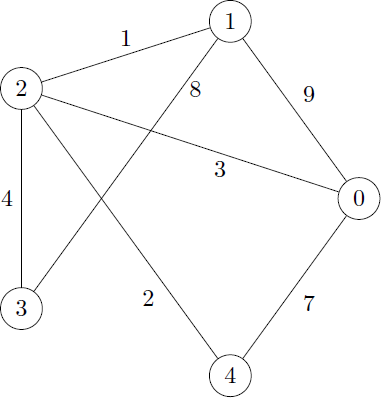
\includegraphics[width=.75\linewidth]{images/exo_3}
\end{center}

\begin{enumerate}
\item Construire la matrice $\left( M_{ij}\right)_{0\leq i,j\leq 4}$, matrice de distances du graphe \texttt{G}, définie par :

<< pour tous les indices $i$, $j$, $M_{ij}$ représente la distance entre les sommets $i$ et $j$,
ou encore la longueur de l'arête reliant les sommets $i$ et $j$ >>.

On convient que, lorsque les sommets ne sont pas reliés, cette distance vaut -1. La distance du
sommet $i$ à lui-même est, bien sûr, égale à 0.
\item Écrire une suite d'instructions permettant de dresser à partir de la matrice \texttt{M} la liste des voisins du sommet 4.
\item Écrire une fonction \texttt{voisins}, d'argument un sommet $i$, renvoyant la liste des voisins du sommet $i$.
\item Écrire une fonction \texttt{degre}, d'argument un sommet $i$, renvoyant le nombre des voisins du sommet $i$, c'est-à-dire le nombre d’arêtes issues de $i$.
\item Écrire une fonction \texttt{longueur}, d’argument une liste \texttt{L} de sommets de \texttt{G}, renvoyant la longueur du trajet d'écrit par cette liste \texttt{L}, c’est-à-dire la somme des longueurs des arêtes empruntées. Si le trajet n'est pas possible, la fonction renverra $-1$.
\end{enumerate}


%\addcontentsline{toc}{subsection}{Exercice 4 -- Gestion de liste}
\subsection*{Exercice 4 -- Gestion de liste}
Soit un entier naturel $n$ non nul et une liste \texttt{t} de longueur $n$ dont les termes valent 0 ou 1. Le but de cet exercice est de trouver le nombre maximal de 0 contigus dans \texttt{t} (c’est-à-dire figurant dans des cases consécutives). Par exemple, le nombre maximal de zéros contigus de la liste \texttt{t1} suivante vaut 4 :
\begin{center}
\begin{tabular}{|c|c|c|c|c|c|c|c|c|}
\hline 
\texttt{i} & 0 & 1 & 2 & 3 & 4 & 5 & 6 & 7 \\
\hline
\texttt{t1[i]} & 0 & 1 & 1 & 1 & 0 & 0 & 0 & 1 \\
\hline
\hline
\texttt{i} & 8 & 9 & 10 & 11 & 12 & 13 & 14 \\
\cline{0-7} 
\texttt{t1[i]} & 0 & 1 & 1 & 0 & 0 & 0 & 0 \\
\cline{0-7}  
\end{tabular}
\end{center}

\begin{enumerate}
\item Écrire une fonction \texttt{nombreZeros(t,i)}, prenant en paramètres une liste \texttt{t}, de longueur n, et un indice i compris entre 0 et $n-1$, et renvoyant :
$$
\left\{
\begin{array}{l}
0, \text{ si } t[i]=1 \\
\text{le  nombre de zéros consécutifs dans t} \\ \text{à partir de t[i] inclus, si t[i] = 0}.
\end{array}
\right.
$$
Par exemple, les appels \texttt{nombreZeros(t1,4)}, \texttt{nombreZeros(t1,1)} et \texttt{nombreZeros(t1,8)} renvoient respectivement les valeurs 3, 0 et 1.
\item Comment obtenir le nombre maximal de zéros contigus d’une liste \texttt{t} connaissant la liste des \texttt{nombreZeros(t,i)} pour $0\leq i \leq n-1$ ?
En déduire une fonction \texttt{nombreZerosMax(t)}, de paramètre \texttt{t}, renvoyant le nombre maximal de 0 contigus d’une liste \texttt{t} non vide. On utilisera la fonction \texttt{nombreZeros}.
\item Quelle est la complexité de la fonction \texttt{nombreZerosMax(t)} construite à la question précédente ?
\item Trouver un moyen simple, toujours en utilisant la fonction \texttt{nombreZeros}, d’obtenir un algorithme plus performant.
\end{enumerate}

%\addcontentsline{toc}{subsection}{Exercice 5 -- Probabilités}
\subsection*{Exercice 5 -- Probabilités}
Soient $n$ un entier naturel strictement positif et $p$ un réel compris entre 0 et 1.
On considère $X$ et $Y$ deux variables aléatoires à valeurs dans $\mathbb{N}$ sur un espace probabilisé donné. $X$ suit une
loi de Poisson de paramètre $\lambda = np$ et $Y$ suit une loi binomiale de paramètres $(n, p)$.

\begin{enumerate}
\item Définir une fonction \texttt{Px}, d’arguments $k$, $n$ et $p$, renvoyant la valeur de $P(X = k)$. $k!$ (factorielle k) s’obtient par \texttt{factorial(k)} en Python (bibliothèque math) et \texttt{prod(1 : k)} en Scilab.
Déterminer, pour $n = 30$ et $p = 0,1$, la liste des valeurs de $P(X = k)$ pour $k \in \mathbb{N}$, $0 \leq k \leq 30 $.
\item Définir une fonction \texttt{Py}, d’arguments $k$, $n$ et $p$, renvoyant la valeur de $P(Y = k)$.
On pourra utiliser \texttt{comb} de la sous-bibliothèque \texttt{scipy.misc} en Python et \texttt{binomial} en Scilab.

Déterminer, pour $n = 30$ et $p = 0,1$, la liste des valeurs de $P(Y = k)$ pour $k \in \mathbb{N}$, $0 \leq k \leq 30$.
\item Soit $k \in \mathbb{N}$. On rappelle que, sous certaines conditions sur $n$ et $p$, la probabilité $P(Y = k)$ peut être
approchée par $P(X = k)$. Déterminer une fonction \texttt{Ecart} d’arguments $n$ et $p$, renvoyant le plus grand
des nombres $|P(Y = k) - P(X = k)|$, pour $0 \leq k \leq n$.
\item Soit $e$ un réel strictement positif. Déterminer une fonction \texttt{N}, d’arguments $e$ et $p$, renvoyant le plus
petit entier $n$ tel que \texttt{Ecart(n, p)} soit inférieur ou égal à $e$.
\item Faire l’application numérique dans les quatre cas suivants :
\begin{itemize}
\item $p = 0,075$ avec $e = 0,008$ et $e = 0,005$;
\item $p = 0,1$ avec $e = 0,008$ et $e = 0,005$. Interpréter le dernier résultat.
\end{itemize}
\end{enumerate}


%\addcontentsline{toc}{subsection}{Exercice 6 -- Tracer de fonction -- $f(x)=0$}
\subsection*{Exercice 6 -- $f(x)=0$}
On considère la fonction $g$ définie sur $[0 , 2[$ par :
$$ g(x) =
\left\{
\begin{array}{ll}
x &\text{ pour } 0\leq x < 1 \\
1 &\text{ pour } 1\leq x < 2 
\end{array}
\right.
$$
\begin{enumerate}
\item Définir la fonction $g$. Tracer sa courbe représentative sur $[0 , 2[$, c’est-à-dire la ligne brisée reliant les points $(x, g(x))$ pour $x$ variant de 0 à 1,99 avec un pas de 0,01.
\item Définir une fonction $f$ donnée de manière récursive sur $[0 , +\infty[$ par :
$$ f(x) =
\left\{
\begin{array}{ll}
g(x) &\text{ pour } 0\leq x < 2 \\
\sqrt{x} f(x-2) &\text{ pour } x \geq 2
\end{array}
\right.
$$
\item Tracer la courbe représentative de $f$ sur $[0,6]$.
\item Écrire les instructions permettant de calculer, à $10^{-2}$ près, la plus petite valeur $\alpha > 0$ telle que $f(\alpha) > 4$.
\end{enumerate}

%\addcontentsline{toc}{subsection}{Exercice 7 -- Algorithmique }
\subsection*{Exercice 7 -- Algorithmique }

On considère le code Python de la fonction \texttt{d} suivante :

\begin{py}
\begin{python}
def d(n):
    L =[1]
    for nombre in range(2,n+1):
        if n%nombre == 0:
            L.append(nombre)
    return L
\end{python}
\end{py}

\begin{enumerate}
\item Quel est le résultat de l’appel \texttt{d(4)} ? Puis de l’appel \texttt{d(10)} ?
Que fait la fonction \texttt{d} ?
\item Un diviseur non-trivial d’un entier \texttt{n} est un diviseur de \texttt{n} différent de 1 et de \texttt{n}. Écrire une fonction \texttt{DNT}, d’argument \texttt{n}, renvoyant la liste des diviseurs non-triviaux de l’entier \texttt{n}.
\item Écrire une fonction \texttt{sommeCarresDNT}, d’argument \texttt{n}, renvoyant la somme des carrés des diviseurs non-triviaux de l’entier \texttt{n}.
\item Écrire la suite des instructions permettant d’afficher tous les nombres entiers inférieurs à 1000 et égaux à la somme des carrés de leurs diviseurs non-triviaux. Que peut-on conjecturer ?
\end{enumerate}

%\addcontentsline{toc}{subsection}{Exercice 8 -- Chiffrer -- déchiffrer}
\subsection*{Exercice 8 -- Chiffrer -- déchiffrer}
Soit n un entier vérifiant $n \leq 26$. On souhaite écrire un programme qui code un mot en décalant chaque lettre de l'alphabet de $n$ lettres.
Par exemple pour $n = 3$, le décalage sera le suivant :
\begin{center}
\begin{tabular}{|l|c|c|c|c|c|c|c|c|c|}
\hline
Avant décalage & a & b & c & ... & x & y & z \\
\hline
Après décalage & d & e & f & ... & a & b & c \\
\hline
\end{tabular}
\end{center}
Le mot \texttt{oralensam} devient ainsi \texttt{rudohqvdp}.
\begin{enumerate}
\item Définir une chaîne de caractères contenant toutes les lettres dans l’ordre alphabétique (caractères en
minuscule).
\item Écrire une fonction \texttt{decalage}, d’argument un entier \texttt{n}, renvoyant une chaîne de caractères contenant
toutes les lettres dans l’ordre alphabétique, décalées de \texttt{n}, comme indiqué ci-dessus.
\item Écrire une fonction \texttt{indices}, d’arguments un caractère \texttt{x} et une chaîne de caractères \texttt{phrase}, renvoyant
une liste contenant les indices de \texttt{x} dans \texttt{phrase} si \texttt{x} est une lettre de phrase et une liste vide sinon.
\item Écrire une fonction codage d’arguments un entier \texttt{n} et une chaîne de caractères \texttt{phrase}, renvoyant
\texttt{phrase} codé avec un décalage de \texttt{n} lettres.
\item Comment peut-on décoder un mot codé ?
\end{enumerate}



%\addcontentsline{toc}{subsection}{Exercice 9 --  Fractale de Mandelbrot}
\subsection*{Exercice 9 -- Fractale de Mandelbrot}

On pose $M = 20$ et $m = 10$. À un nombre $c$ quelconque, on associe la suite $(u_n)_{n\geq 0}$ définie par $u_0 = 0$ et $u_{n+1} = u_n^2 + c$ pour $n \geq 0$.

S’il existe, on note $k$ le plus petit entier tel que l’on ait $0 \leq k \leq m$ et $|u_k| > M$.
On définit alors la fonction $f$ par 
$$
f : c \mapsto 
\left\{
\begin{array}{l}
k \text{ s'il existe} \\
m+1  \text{ sinon.}
\end{array}
\right.
$$

\begin{enumerate}
\item  Donner le code définissant la fonction $f$.
\item  Tracer l’allure de la courbe représentative de la fonction $f$ sur $[-2; 2]$, en créant une liste \texttt{LX} de 401 valeurs équiréparties entre -2 et 2 inclus et en utilisant les fonctions \texttt{plot} et show de la sous-bibliothèque \texttt{matplotlib.pyplot}.
\item  Construire le tableau des valeurs $f(x+i y)$ où $x$ prend 101 valeurs comprises entre -2 et 0,5 et $y$ prend
101 valeurs entre -1,1 et 1,1. \textit{On rappelle que le nombre complexe $i$ est représenté par $1j$. Par exemple,
le complexe $1 + 2 i$ est représenté par $1+2j$.}
\item  Tracer l’image que code ce tableau. On pourra utiliser les fonctions \texttt{imshow} et \texttt{show} de la sous-
bibliothèque \texttt{matplotlib.pyplot}. Quels paramètres peut-on modifier pour obtenir une meilleure résolution ?
\end{enumerate}


%\addcontentsline{toc}{subsection}{Exercice 10 -- Calcul matriciel}
\subsection*{Exercice 10 -- Calcul matriciel}
\textit{Dans cet exercice, avec Python on pourra utiliser la fonction \texttt{array} de la bibliothèque \texttt{numpy}, ainsi que la
fonction \texttt{eig} de la sous-bibliothèque \texttt{numpy.linalg}. Avec Scilab, on utilisera \texttt{spec}.}

\begin{enumerate}
\item Créer deux matrices $R=\begin{pmatrix} 1 & 2 & 3 \\ 4 & 5 & 6  \end{pmatrix}$ et 
$S =\begin{pmatrix} 1 & 2 & 3 \\ 4 & 5 & 6\\ 7 & 8 & 9  \end{pmatrix}$ et les faire afficher.
\item Créer une fonction \texttt{test}, d’argument $M$, renvoyant la valeur \texttt{n} si $M$ est une matrice carrée d’ordre \texttt{n} (entier naturel non nul) et zéro dans tous les autres cas.
Vérifier la fonction test sur $R$ et sur $S$.
\item Le fichier \texttt{ex\_006.txt}, situé dans le sous-répertoire \texttt{data} du répertoire de travail, contient un tableau de valeurs flottantes. Lire ce tableau dans le fichier et vérifier qu’il correspond bien à une matrice carrée d’ordre 5 que l’on désignera par \texttt{M1}. 
\item Déterminer les valeurs propres de la matrice \texttt{M1}.
\item Créer une fonction \texttt{dansIntervalle}, d’arguments une liste $L$ et deux réels $a$ et $b$, renvoyant la valeur \texttt{True} si tous les éléments de la liste $L$ sont dans l’intervalle $[a, b]$ et \texttt{False} sinon. Vérifier que toutes les valeurs propres de la matrice \texttt{M1} sont dans l’intervalle $[0, 1]$.
\end{enumerate}


%\addcontentsline{toc}{subsection}{Exercice 11 -- Tri de liste}
\subsection*{Exercice 11 -- Tri de liste}
Soit $N$ un entier naturel non nul. On cherche à trier une liste L d’entiers naturels strictement inférieurs à $N$.
\begin{enumerate}
\item Écrire une fonction comptage, d’arguments $L$ et $N$, renvoyant une liste $P$ dont le $k$-ième élément désigne le nombre d’occurences de l’entier $k$ dans la liste $L$.
\item Utiliser la liste $P$ pour en déduire une fonction \texttt{tri}, d’arguments $L$ et $N$, renvoyant la liste $L$ triée dans l’ordre croissant.
\item Tester la fonction \texttt{tri} sur une liste de 20 entiers inférieurs ou égaux à 5, tirés aléatoirement.
\item Quelle est la complexité temporelle de cet algorithme ? La comparer à la complexité d’un tri par insertion ou d’un tri fusion.
\end{enumerate}

%\addcontentsline{toc}{subsection}{Exercice 12 -- Courbes paramétrées}
\subsection*{Exercice 12 -- Courbes paramétrées}
\begin{enumerate}
\item Deux paramètres $b$ et $w$ valant respectivement 0,5 et 6,0, définir trois fonctions d’une variable $t$ renvoyant des couples :
$$
\left\{
\begin{array}{ll}
p : t \mapsto &\left(\cos(t) +b \cos(wt),      \sin(t) + b \sin (wt) \right) \\
v : t \mapsto &\left(-\sin(t)  -bw \sin(wt),\right. \\     
& \quad \left. \cos(t) + b w\cos (wt) \right) \\
a : t \mapsto &\left(-\cos(t)-bw^2 \cos(wt),\right. \\ 
& \quad \left.-\sin(t) - b w^2 \sin (wt) \right) \\
\end{array}
\right.
$$
Vérifier ces fonctions sur un exemple.

$p(t)=(x(t),y(t))$ désigne la position dans le plan d'une masse ponctuelle mobile au cours du temps, $v(t)=(x'(t),y'(t))$, sa vitesse, et $a(t)=(x''(t),y''(t))$, son accélération.
\item Construire la liste \texttt{L} des points $p(t)$, pour $t$ variant de $-\pi$ à $\pi$ avec un pas de discrétisation $\delta t$ vérifiant $\delta t = 0,01 \; \pi$.
\item Faire tracer dans le plan muni d’un repère orthonormal la ligne polygonale reliant les points $p(t)$ de la liste \texttt{L}.
\item Définir puis tester la fonction $c$ d’une variable $t$ qui renvoie le couple des coordonnées du centre de courbure donnée par :
$$
c(t)=\left(x(t)-dy'(t),y(t)+dx'(t)\right) $$ 
où
$$
d= \dfrac{x'(t)^2+y'(t)^2}{x'(t)y''(t)-y'(t)x''(t)}.
$$
\item Rajouter sur le graphique précédent la ligne décrite par les centres de courbure, avec la même
discrétisation en temps.
\item Calculer la longueur de la ligne polygonale reliant les points $p(t)$, pour différents pas de discrétisation $\delta t$. Observer l'évolution de cette longueur lorsque $\delta t$ diminue.
\end{enumerate}
\end{multicols}




\newpage

\section{Exercices de la banque PT -- 2017 -- À vérifier}

\begin{multicols}{2}

\subsection*{Exercice 1}
\textit{Exercice tombé 2 fois.}
\begin{enumerate}
\item Écrire une fonction \texttt{C1} d'argument $n$ qui contient les carrés parfaits inférieurs ou égal à $n$. (Par exemple : \texttt{C1 (10) =[0,1,4,9]}.) Afficher C1 (100). 

\item Écrire une fonction \texttt{C2} d'argument $n$ qui contient la somme de deux carrés parfaits inférieurs ou égal à $n$. La liste doit être triée. Afficher \texttt{C2 (100)}.

\item Soit $m= p^2 + q^2$. Écrire une fonction \texttt{decomp} d'argument $m$ qui renvoie les couples $p$ et $q$ tel que $m= p^2 + q^2$. 

\item Écrire une fonction \texttt{C3} d'argument $n$ qui renvoie la somme de trois carrés parfaits inférieurs ou égal à $n$. La liste doit être triée. \texttt{Afficher C3 (100)}.

\item  Montrer que tous les entiers inférieurs ou égal à 2016 qui ne s'écrivent pas comme la somme de 3 carrés parfaits sont de la forme : $4^k  (8q+7)$. 
\end{enumerate}


\subsection*{Exercice 2}
\begin{enumerate}
\item Si \texttt{M=[[0,0,0],[0,x,0],[0,0,0]]}, 

\texttt{UnAnDePlus(M)} renvoie 
\texttt{[[0,0.1*x,0]}, \texttt{[0.05*x,1.3*x,0.2*x]}, \texttt{[0,0.1*x,0]]}. 

Tester votre programme sur 10 ans avec la matrice $M$ donnée.


%def UnAnDePlus(M):
%    m,n=len(M),len(M[0])
%    M2=[[0 for j in range (n)]for i in range (m)]
%    for i in range (m):
%        for j in range (n):
%            M2[i][j] += M[i][j]*1.3
%            if i-1>0:                       # Nord
%                M2[i-1][j] += M[i][j]*0.1
%            if i+1< m :                     # Sud
%                M2[i+1][j] =+ M[i][j]*0.1
%            if j-1>0:                       # Ouest
%                M2[i][j-1] +=M[i][j]*0.05
%            if j+1 < n:                     # Est
%                M2[i][j+1] += M[i][j]*0.2
%    for i in range (m):
%        for j in range (n):            
%                if M2[i][j] > 1:
%                    M2[i][j]=1
%    return (M2)
                
    
\item En réalité, toutes les zones ne sont pas aussi propices pour l'espèce. On donne une matrice $S$ de saturation, le taux de présence de l'espèce à la case $i,j$ doit être inférieur à $S[i][j]$.
Adapter l'algorithme.

%# on change la fin   
%#     for i in range (m):
%#         for j in range (n):            
%#                 if M2[i][j] > S[i][j]:
%#                     M2[i][j]=S[i][j]

\item $S$ est stocké dans le répertoire data dans le fichier \texttt{lessaturation.txt}, les valeurs sont séparées par des espaces. Extraire $S$.

\item On suppose que $M$ est de taille $m\times n$, à la case $(60,30)$ il y a la proportion $x=0,01$ la première année, afficher la propagation au bout de 100 ans (on utilisera \texttt{imshow} dans la bibliothèque \texttt{matplotlib}).

\end{enumerate}

\subsection*{Exercice 3}

On définit un segment ainsi : \texttt{[a,b]}.
\begin{enumerate}
\item Écrire une fonction \texttt{disjoints} qui prend pour argument deux segments et qui permet de savoir si deux segments sont disjoints. 
\item Écrire une fonction \texttt{fusion} qui prend pour argument deux segments et qui les rassemble. (La borne inférieure est le minimum des deux segments et la borne supérieure le maximum).
Une liste est correctement formée si cette liste est composée de segments disjoints deux à deux et classés dans l’ordre croissant. 
\item Ces listes sont-elles correctement formées ? 
\texttt{L1= [[1,2],[3,5],[4,6]]}, 
\texttt{L2= [[1,2],[5,6],[3,4]]}, 
\texttt{L3= [[1,2],[3,4],[5,6]]}.
\item Écrire une fonction récursive vérifie qui prend pour argument une liste et qui permet de savoir si une liste de segments est correctement formée. 
\item Créer une fonction appartient qui prends pour argument \texttt{x} (un nombre) et \texttt{L} (une liste de segment) et qui renvoie \texttt{True} si \texttt{x} appartient à un des segments. 
(Par exemple 1,5 appartient à \texttt{L3}).

\end{enumerate}
%Corrigé à mettre en forme. 

%Q1)
%def disjoints(s1,s2) :
%	if s1[0]>s2[1] :
%		return(True)
%	Elif s1[1]<s2[0] :
%		Return(True)
%	Else :
%		Return (False)
%
%def fusion(s1,s2) :
%	if s1[0]<s2[0] :
%		inf = s1[0]
%	else :
%		inf = s2[0]
%	if s1[1]>s2[1] :
%		sup = s1[1]
%	else :
%		sup=s2[1]
%	return ([inf,sup])
%
%Q3) non-non-oui
%Q4)
%def verifie (L) :
%	if len(L)==1
%		return(True)
%	else :
%		L2=L[1 :]
%		return(disjoints(L[0],L2[0]) and L[0][1] > L2[0][0] and verifie(L2))
%Q5)
%def appartient (x,L) :
%	s=0
%	for i in range (len(L)) :
%		for j in range(len(L[i])-1) :
%			if L[i][j] <= x < L[i][j+1] :
%				s=1
%	return(s==1)
%


\subsection*{Exercice 5}
\begin{enumerate}
\item Écrire une fonction "avec" d'arguments deux entiers non nuls $k$ et $n$, renvoyant une liste d'un tirage de $k$ entiers compris entre $0$ et $n-1$ déterminés aléatoirement (en utilisant \texttt{randint}). Le tirage se fait avec remise.
\item Même question sans remise.
\item La fonction à écrire doit renvoyer une matrice (liste de liste) de la forme suivante en plaçant aléatoirement 0,1... 9 :
$$
\begin{pmatrix}
\star & \star & 2& \star & \star \\
3 & 4 & 5 & \star & \star \\
\star & \star & 9 & \star & \star \\
\star & 1 & \star & \star & 0 \\
8 & \star & 6 & 7 & \star \\
\end{pmatrix}
$$
\end{enumerate}

\subsection*{Exercice 6}
On note $E_n=\left\{1,...,b\right\}$. Dans Python, on note les parties de $E_n$ comme des listes. Ainsi, on note $\{0 \}$, $\{ 2\}$, $\{(3,4) \}$ respectivement \texttt{[[]]}, \texttt{[[2]]}, \texttt{[[3,4]]}.   

\begin{python}
def A (listes,numero):
    res = []
    for L in listes :
        res.append(L+[numero])
    return(res)
\end{python}
\begin{enumerate}
\item Expliquer ce que fait la fonction $A$. Donner notamment la nature de l'argument listes. 
\item Donner L0, le nombre de parties de $E_5$ à 0 élément.
\item Écrire la fonction récursive parties, d'argument $n$ et $p$, renvoyant le nombre de parties de $E_n$ d'au plus $p$ éléments.  \textit{On pourra remarquer que l'ensemble des parties de $E_n$ à $p$ éléments contenants $n$ et les parties de $E_n$ à $p$ éléments ne contenant pas $n$ réalisent une partition de $E_n$? On pourra traiter à part les cas $n=0$ et $p=0$.}
\item Déterminer $L_1$ l'ensemble des parties de $E_5$ à 1 élément.
\item Déterminer $L_5$ l'ensemble des parties de $E_5$ à 5 éléments.
\item Écrire une fonction récursive parties2 d'arguments $n$ et $p$ renvoyant le nombre de parties de $E_n$ avec exactement $p$ éléments.
\end{enumerate}

%Quelques points de correction :
%def parties (n,p) :
%    """ renvoie les parties de En d'au plus p élements """
%    if p == 0 :
%        return(L0)
%    if n == 0 :
%        return(L0)
%    else :
%        res1 = parties(n-1,p)
%        res2 = parties(n-1,p-1)
%        return(res1 + A(res2,n))
%    
%def parties2v1 (n,p) :
%    """ renvoie les parties de En avec exactement p élements """
%    
%    partie = parties(n,p)
%    res = []
%    
%    for el in partie :
%        if len(el) == p :
%            res.append(el)
%
%    return(res)
%
%def parties2v2 (n,p) :
%    """ renvoie les parties de En avec exactement p élements """
%    
%    partiep1 = parties(n,p-1)
%    res = partiep [:]
%
%    for el in res :
%        for el1 in partiep1 :
%            if el == el1 :
%                res.remove(el)
%

\subsection*{Exercice 7}
Il fallait générer un jeu de 32 cartes à partir des listes valeurs=["7","8","9","10","V","D","R","A"] et couleurs=["T","K","C","P"].
Ensuite je devais définir la fonction \texttt{tirermain} permettant de tirer une main de 5 cartes (à l'aide de la fonction \texttt{sample} de la bibliothèque \texttt{random}).
La troisième question consistait en la définition d'une fonction \texttt{LV} d'argument une main qui renvoyait une liste triée par ordre croissant du nombre de fois qu'une valeur apparaissait dans la main.
Par exemple, si la main contient une double paire, LV doit renvoyer [1,2,2]
Si la main contient un brelan, LV doit renvoyer [1,1,3]
Pour trier la liste, on avait le droit d'utiliser la fonction \texttt{sorted}.
Je devais ensuite calculer la probabilité d'obtenir une paire, une double paire, un full (une paire et  un brelan) et un carré, en faisant un test sur 5000 mains.

\subsection*{Exercice 8}
L'exercice traitait du chemin d'une fourmi sur un quadrillage, à chaque instant la fourmi pouvait se déplace dans les 4 directions possibles.

\begin{enumerate}
\item Créer une fonction renvoyant aléatoirement une des 4 listes suivantes : $[0,1] , [1,0] , [-1,0] , [0,-1]$  (fonction sans argument)
on pourra utiliser la bibliothèque random.
\item Créer une fonction chemin renvoyant un chemin jusqu'à que la fourmi sorte du carré défini par $-2< x < 2$ et $-2 < y < 2$ (elle part de l'origine donc $[0,0]$).
 
%# J'ai eu des problème de copie de liste dans cette question , je renvoyait une liste avec les coordonnés de touts les points parcouru au cours du chemin mais celle si se modifiait au fur et a mesure en renvoyait les coordonnées du dernier point à la place de chaque point intermédiaire. D'autant plus que l'examinatrice ne comprenait pas l'origine du problème j'ai finalement trouvé la solution seul mais j'ai perdu trop de temps

\item Tracer 6 chemin différents pour une fourmi dans un carré  $-10< x < 10$ et $-10 < y < 10$.
\end{enumerate}

\subsection*{Exercice 9}
\textit{
Mon oral d'info portait sur la répartition de population.
Je devais d'abord expliquer un premier programme qui créait une liste de complexes x + jy  de manière aléatoire.
Je devais afficher les points sur un graphe ( j'avais besoin des fonctions .imag et . reel ( je ne sais plus exactement ) que je ne connaissais pas ) 
Ensuite, il fallait que je trouve l'habitation où devait se passer une réunion : le trajet devait être le minimum des maximum de chemin pour chacune des maisons ( c'est plutôt compliqué à expliquer j'ai mis un moment à comprendre l'énoncé ) 
Je me suis arrêtée là
En fait, il m'a paru plus dur de comprendre l'énoncé que de réaliser le programme.
De plus, on est pas habitué à utiliser les fonctions usuelles comme max,min...  je n'ai pas eu le reflex de les utiliser.}


\subsection*{Exercice 10}
On appelle un intervalle une liste de 2 éléments $[a,b]$ tel que $a <b$.

\begin{enumerate}
\item Créer une fonction disjoints de paramètres i1 et i2 2 intervalles qui renvoie True si les deux intervalles sont disjoints ou False sinon.
\item Créer une fonction fusion qui renvoie un intervalle $[a,b]$ tel que $a$ est le minimum de i1 et i2, et b le max.
\item On considère une liste d intervalle l=[i1,i2,i3...]. Elle est considérée "juste" si les intervalles vérifient 2 à 2 :
\begin{itemize}
\item ils sont disjoints 2 à 2;
\item ils sont croissant, ie le max du précédent est inférieur strict au minimum du suivant.
\end{itemize}

Écrire une fonction récursive juste de paramètres L qui renvoie True si cette liste d'intervalle est juste ou False sinon.
\end{enumerate}


\subsection*{Exercice 11}

\begin{enumerate}
\item Définir une fonction polynomiale \texttt{q(x,y)} classique à deux variables.
\item Définir une fonction renvoyant un tableau(matrice) de paramètre \texttt{e}.
\item On a une fonction \texttt{p(x,y)} continue sur un intervalle, modélisation de la fonction par une avancée de triangles. Si la fonction \texttt{p(x,y)} entre dans le triangle ABC par AB alors $p(xa,xb)\cdot p(ya,yb)\leq 0$ et elle rentre dans un autre triangle (on conserve les points qui tracent le segment d'entrée et le point restant est le symétrique du 3e point par rapport au segment d'entrée) et ainsi de suite.
\end{enumerate}


\subsection*{Exercice 12}

\begin{enumerate}
\item Tester deux lignes de commandes (elles permettaient de transformer un entier en la liste des nombres sous forme de caractères , ou quelque chose comme ça et inversement )  
\item À partir de ça, créer une fonction \texttt{R(n)} qui renvoie la retournée de \texttt{n}. (La retournée de 13 est 31, celle de 140 est 41 par exemple.)
\item Créer une fonction qui renvoie la distance entre un nombre et sa retournée.
\item Créer une fonction de paramètres \texttt{(a,N)} qui renvoie les \texttt{N+1} termes de la suite $u_{n+1}=R(u_n), u_0=a$    (je ne sais plus si c’est la suite des retournées ou la suite des distances entre retournées … mais je penche plus pour le deuxième).
\item Trouver le plus petit a tel que $u_{20}= 0$.
\item Trouver la liste des $a$ entre 1000 et 10000 tels que $u_{20}= 0$ (pas sûr non plus).
\item Vérifier que la suite un est 2-périodique à partir d’un certain rang et qu’elle oscille entre les valeurs …. Et …. (en gros, ces deux valeurs sont retournées l’une de l’autre, donc dès qu’on en atteint une, la suite est limitée à ces deux valeurs ).
\end{enumerate}

\subsection*{Exercice 13}

On s’intéresse ici au codage d’un mot. On note A l’alphabet, M le message à coder et k la clé du code. Le message est codé si chaque lettre du mot de base est décalée de k places vers la droite dans l’alphabet A.
Si un caractère du message de base n’est pas dans l’alphabet A, le codage de modifie pas le dit-caractère.

\begin{enumerate}
\item Créer la chaine de caractère suivante : \texttt{mnsc = ‘abcdefghijklmnopqrstuvwxyz’}.
\item Vérifier qu’il y a bien 26 caractères.
\item Créer une fonction \texttt{codee} d’arguments A, M, k renvoyant le message M codé.
\item Comment obtenir le mot de base connaissant la clé k d’un mot codé ?
\item On dispose d’un fichier txt contenant un message codé. On ignore la clé de ce message
Quelle est le caractère le plus fréquent dans ce message ?
\end{enumerate}

\subsection*{Exercice 14}
$(u_n)$ definie par $u_0=1$ et et $u_{n+1}= f(u_n)$ où 
$$
\begin{array}{rcl}
f : [1,1] & \rightarrow  & [2,1] \\
\big[  1,1,1,2,1 \big]  & \rightarrow &  [3,1,1,2,1,1] \\
\end{array}
$$
renvoie le nombre d'apparitions consécutives d'un élément + cet élément.
\begin{enumerate}
\item Écrire une fonction lire d'argument une liste \texttt{L} renvoyant \texttt{f(L)}. Afficher \texttt{lire([1,1,2,2,1])}.
\item Que fait la fonction \texttt{L2str} :
\begin{python}
def  L2str(L) :
    ch='' ''
    for e in L :
        ch=ch+str(e)
    return (ch)
\end{python}
\item Afficher les 15 premiers termes de $u_n$. Quels nombres apparaissent ?
\end{enumerate}


\subsection*{Exercice 15}

Il y avait un graphe exemple. Un graphe est défini par une liste de tuples. Un tuple est une arrête: c'est le numéro des deux sommets qu'elle relie.

Par exemple: \texttt{L=[(0,1),(1,2),(4,1),(0,1)]}.

\begin{enumerate}
\item Le degré d'un sommet est son nombre de voisin. Écrire une fonction \texttt{degre} d'arguments une liste L et un entier k qui renvoie le degré du sommet numéro k du graphe définit par la liste L.
\item Un sommet est dit non isolé si il n'a pas de voisin. Écrire une fonction \texttt{non\_isole} d'argument L qui renvoie le nombre de sommets non isolé du graphe définit par L.
\item La liste d'adjacence d'un graphe est une liste de liste. Ainsi l'élément d'indice k est la liste des voisins du sommet numéro k.
Écrire une fonction \texttt{adjacance} d'arguments L et n le nombre de sommets du graphe et qui renvoie la liste A d'adjacence du graphe.

Pour l'exemple initial, on a A=[[1],[0,2,4],[1,4],[],[1,2]].

\item Écrire une fonction \texttt{deg\_max} d'argument A la liste d'adjacence d'un graphe et qui renvoie le numéro du sommet ayant le plus haut degré. (Je crois qu'il fallait renvoyer le numéro du sommet et pas le degré maximal mais je ne suis pas très sûr).
\end{enumerate}

\subsection*{Exercice 16}

Soit $u_n$ une suite définie par $u_{n+3}=2u_{n+2}+u_{n+1} - u_n$. Soit $P$ un polynôme défini par $P=X^3-2X^2-X+1$. $u_n=a\lambda^n+b\mu^n+ c\nu ^n$, $|\lambda|>|\mu|>|\nu|$ avec $\lambda$, $\mu$, $\nu$ racines de $P$.
\begin{enumerate}
\item Écrire une fonction \texttt{f(N,x,y,z)} affichant les $N$ premiers termes de $u_n$ dans une liste sachant que $(x,y,z)$ sont les trois premiers termes. Test par $N=10$, $x=1$, $y=2$, $z=3$.
\item À l'aide de $\dfrac{u_{n+1}}{u_n}$, trouver $\lambda$ tel que $P$ soit inférieur à $10^{-10}$.
\item Soit $Q(x)=X^3P\left(\dfrac{1}{X}\right)$. Trouver $r$ tel que $Q$ soit inférieur à $10^{-10}$.
\item Trouver $\mu$.
\end{enumerate}

\subsection*{Exercice 17}
Écrire les fonctions permettant de transformer la liste $[0,0,1,1,1,0,0,1,1]$ :
\begin{itemize}
\item en $[2,5,6,8]$ (places des coupures);
\item en $[2,0,3,1,1,0,2,1]$.
\end{itemize}

\subsection*{Exercice 18}

On modélise un pendule pesant. On a une masse au bout d’une corde, on note $\alpha$ son angle avec la verticale.
On donne l’équation vérifiée par $\alpha$ :
$$\begin{array}{c}
\alpha '' = - m \alpha  - f \alpha   (m \text{ et } f \text{ sont donnés}) \\
\alpha (0) = 0 \, \text{rad} \\
\alpha'(0) = \omega_0 rad / s (on lance la masse avec une vitesse initiale qui sera préciser après je crois)\\
\end{array}
$$
Question à faire sur le brouillon : 
on note $u(t) = (\alpha, \alpha')$ donner $\psi(u(t)) = u’(t)$.

\begin{enumerate}
\item Résoudre le système avec « odeint ».

\item Tracer la courbe de $\alpha$ en fonction du temps (avec $\omega_0 =$1 ; 2 ; 4 ; 8 rad/s ).

\item Pourquoi $\alpha$(infini) = cste qui dépend de $\omega_0$ ?
\end{enumerate}

\subsection*{Exercice 19}
$$ A= \begin{pmatrix}
2 & 4 & 6 & 9 \\
11 & 13 & 15 & 17 \\
27 & 29 & 31 & 33 \\
47 & 49 & 51 & 53 \\
\end{pmatrix}$$

Soit $P$ un polynôme tel que $P(X)=a_n X^n + a_{n-1}X^{n-1} + ... + a_1 X + a_0$. Soit la suite des $(B_k)$ telle que $\left\{ \begin{array}{c} B_0 = M \\ B_{k+1} = M\left( B_k - \dfrac{Tr(B_k)}{k+1} I\right)\end{array}\right.$. On note $Q(x)=X^n - \sum \limits^n_{k=1}  \dfrac{Tr(B_{k-1})}{k}X^{n-k}$. $L=[a_n,a_{n-1},...;a_1,a_0]$.

\begin{enumerate}
\item Définir une fonction \texttt{valpol} d’arguments la liste $L$ et $x$ et qui renvoie $P(x)$. 
\item Écrire la matrice $A$.
\item Calculer $A(A-Tr(A)I_4)$.
\item Définir une fonction \texttt{pol} d’argument $M$ et qui renvoie une liste associée à Q(X).
\item Obtenir pol(A)
\item Tracer la courbe des Pol(A) pour x variant de -5 à 1.5.
\end{enumerate}


\subsection*{Exercice 20}
\textit{
Il fallait créer 2 matrices 2*2.
Pour créer les coefficients, il fallait ouvrir un tableur .csv .
À partir de ces valeurs, la création des coefficients des matrices était facile (carrés, multiplications ....)
Il fallait ensuite résoudre le système matriciel AX = B grâce à linealg de scipy, je n'y ai pas pensé tout de suite et j' ai commencé à écrire la méthode du pivot ....}


\subsection*{Exercice 21}

Dans une liste de longueur n, un élément est dit majoritaire si le nombre d’occurrences de cet élément est strictement supérieur à n/2.
\begin{enumerate}
\item Créer une fonction d’argument une liste L et un élément x renvoyant le nombre d’occurrences de x dans L.
\item Créer une fonction \texttt{maj(L)} renvoyant le nombre d’éléments majoritaires dans la liste L ainsi que leur nombre d’occurrences respectifs. La fonction renverra [0,-1] s’il n’y a aucun élément majoritaire.
\item Soient deux listes L1 et L2 extraites d’une liste L. Montrer, sur papier, que si un élément de L est majoritaire, alors il l’est également dans l’une des deux listes L1 et L2.
\item  Lire le fichier  « valeurs.csv ». Il contient un tableau de valeurs à deux colonnes. Les deux colonnes ont le même nombre de lignes. Déterminer le nombre de lignes dans chaque colonne.
\end{enumerate}



\subsection*{Exercice 22}

\begin{enumerate}
\item Écrire une fonction partage d’arguments une liste L et a un nombre. Pour tous les éléments de L, si l’élément est strictement plus petit qu’a, on l’ajoute à Linf ; si l’élément est supérieur ou égal à a, on l’ajoute à Lsup. La fonction renvoie, Linf et Lsup.
\item Écrire le quick sort (vraiment rédiger comme cela sans rien de plus)
\item Implanter un retour de nombre de comparaisons.
\item Tester le tri avec une liste de 40 000 éléments aléatoires entre -999 et 999.
\end{enumerate}
\end{multicols}

%Hugo SCHINDLER
%# Oral de mathématiques 2017
%from random import randint
%#Question 1
%def partage(L, a): Linf=[] Lsup=[] for i in L: if i<a: Linf.append(i) else : Lsup.append(i) return Linf, Lsup
%""" Lt=[0, 2, 8, 3, 6, 7] at=2 print(partage(Lt, at)) """
%#Question 2
%def partageQ(L, a): Linf=[] Lsup=[] La=[] for i in L: if i<a: Linf.append(i) else : if i>a: Lsup.append(i) else : # i==a
%La.append(i) return Linf, La, Lsup
%def Quicksort(L): if len(L)<=1: return L else : pivot=L[randint(0, len(L)-1)] Linf, La, Lsup=partageQ(L, pivot) return Quicksort(Linf)+La+Quicksort(Lsup) """ Lt=[0, 2, 8, 3, 6, 7, 2, 8, 0] print(Quicksort(Lt)) """
%#Question 3
%def QuicksortO(L): if len(L)<=1: return L, 1 else : pivot=L[randint(0, len(L)-1)] Linf, La, Lsup=partageQ(L, pivot) L1, n1=QuicksortO(Linf) L2, n2=QuicksortO(Lsup) return L1+La+L2, 3*len(L)+n1+n2 """ Lt=[0, 2, 8, 3, 6, 7, 2, 8, 0] print(QuicksortO(Lt)) """
%#Question 4
%LT=[] for i in range(40000): LT.append(randint(-999, 999)) print(QuicksortO(LT)[1])
\newpage


\section{Exercices de l'oral de Polytechnique -- 2017 -- À vérifier}

\begin{multicols}{2}

\subsection*{Exercice 1}

Les listes sont de tailles supérieures ou égales à 3 et composées d’éléments distincts.
\begin{enumerate}
\item Écrire une fonction \texttt{maxi} d’argument une liste \texttt{lst} de taille $n$ qui renvoie le maximum de \texttt{lst} en effectuant $n-1$ comparaisons.
\item Écrire une fonction \texttt{maxmin} d’argument une liste \texttt{lst} de taille $n$ qui renvoie le couple \texttt{(max, min)} en effectuant $3/2n+1$ comparaisons.
\item Écrire une fonction \texttt{ord\_triee} d’argument \texttt{k} et une liste \texttt{lst} qui renvoie l’élément \texttt{x} de la liste \texttt{lst} triée tel que $x$ possède $k$ éléments plus petit que lui. Ainsi le minimum est \texttt{ord\_triee (0, lst)} le maximum \texttt{ord\_triee (n-1, lst)}. Écrire une fonction \texttt{ord\_naif} d’argument \texttt{k} et une liste \texttt{lst} qui renvoie l’élément \texttt{x} de la liste \texttt{lst} non triée tel que \texttt{x} possède \texttt{k} éléments plus petit que lui.
\item Écrire une fonction récursive \texttt{ord1(k, lst)} effectuant la même chose que précédemment. Un algorithme est donné :
\begin{itemize}
\item on sépare la liste \texttt{lst} en 2 listes : une liste de valeurs plus grande que le 1\ier élément, une liste de valeurs plus petite que le 1\ier élément;
\item trouver la condition d’arrêt et d’appel récursif
\item donner la complexité si on exécute \texttt{ord1(N-1, L)} avec la liste \texttt{L=[0, 1, 2, 3, …. N]}.
\end{itemize}
\item Écrire une fonction récursive \texttt{select(k, lst)} effectuant la même chose que précédemment. On améliore l’algorithme précédent. Un algorithme est donné : 
\begin{itemize}
\item on sépare la liste en liste de 5 éléments avec la dernière liste de taille au plus égale à 5. On appelle la liste de liste segment
\item on calcule la médiane de chaque petite liste. On obtient un tableau de médianes $M$;
\item on calcule la médiane des médianes : $mdm$,
\item on sépare la liste \texttt{lst} en 2 listes : une liste de valeurs plus grande que la médiane des médianes, une liste de valeurs plus petite que la médiane des médianes,
\item trouver la condition d’arrêt et d’appel récursif.
\end{itemize}
\item Montrer qu’il existe 1/2*3/5*n-7 éléments plus grand que la médiane des médianes. Montrer qu’il existe 1/2*3/5*n-7 éléments plus petit que la médiane des médianes.
\item Montrer que le nombre d’opérations $T(n)$ effectués par select s’écrit :
\begin{enumerate}
\item $T(n)<A si n<140$;
\item $T(n)<B*n+T(7/10*n)+T(n/5) si n>=140$. (Ne pas déterminer A et B).
\end{enumerate}
\item En déduire la complexité de select.
\item Modifier le programme select pour qu’il gère les listes avec des éléments non distincts
\end{enumerate}

\subsection*{Exercice 2}
Épreuve : 1H de préparation, 45 min de présentation orale.

Soit $M$ une matrice de taille $n\times m$. On considère que $M$ est triée si : 
$$
\left\{
\begin{array}{c}
M[i,j] \leq M[i+1,j] \quad 0\leq i \leq n-1  \\
M[i,j] \leq M[i,j+1] \quad 0\leq j \leq m-1 
\end{array}
\right.
$$

($M$ est triée par ligne et par colonne, $M[0,0]$ est la plus petite valeur de $M$ et $M[n-1,m-1]$ la plus grande). 
L'épreuve consiste à trouver différentes façon de rechercher un élément dans un tableau (trié ou non).


\begin{enumerate}
\item Créer une fonction \texttt{est-Trié(M)} qui renvoie \texttt{True} quand le tableau est trié, \texttt{False} sinon. Quelle est la complexité ?

%J'ai parcouru toutes les lignes en vérifiant la condition, si la condition n'est pas vérifiée, je renvoie False (fin de l'algo)
%Ensuite je fais la même chose mais sur les colonnes (les examinateurs m'ont dit de passer à la suite) à la fin, si je ne suis pas sorti de l'algo, je renvoie True. (O (n*m))


\item Donner une méthode pour avoir une matrice triée.

%J'ai eu du mal à cette question, je suis partie sur quelquechose de compliquée (j'avais donc passé cette question et suis revenu, à la fin, dessus pendant les 1H de préparation)

%L'idée était de créer une liste où l'on met tous les élements de la matrice, on trie ensuite cette liste (il m'ont posé des question sur le trie fusion, son principe de fonctionnement, sa complexité) on complète alors la première ligne d'une autre matrice de taille n*m avec les n premier termes de la liste, puis on met les n suivants sur la 2ème ligne de la matrice...


\item On pose $l= 1 ! \times  2 ! \times  ...\times  (n-1) ! \times  n ! \times (n-1) !\times  ...\times 1$. Soit $M = (a_{ij}) \quad  0 \leq i \leq n-1$;  $0<= j \leq n-1$; avec les $a_{ij}$ distincts et  $0 \leq a_{ij} \leq  n\times n$. Montrer qu'il existe $l$ matrices triées et distinctes.

%on donnait dans le cas n=6    
%cas n=4 (moins long)  
%M=[    [1,3,6,10]
%	[2,5,9,13]
%	[4,8,12,15]
%	[7,11,14,16]]
% On remarque qu'on peut permuter les élement d'une diagonale en gardant une matrice triée.
%D'où les l possiblitées.

\item Recherche d'un élément dans une matrice quelconque. Peut on avoir une complexité linéaire ?

%L'algo (primitif) consiste à regarder chaque élément de M et le comparer à x (valeur recherché)
%def recherche (M,x) :  ...

%Il me semble avoir expliqué à l'oral ce que faisait l'algorithme sans l'écrire.
\begin{rem}Beaucoup de question ici, il fallait prouver que si l'algorithme ne regardait pas les $n\times m$ cases de $M$, il ne pouvait pas conclure de manière certaine que $x$ était dans la matrice ou non. ($M$ quelconque). 

J'avais du mal à comprendre la question, la réponse me paraissait évidente. Il fallait dire que si une case n'est de façon certaine pas prise en compte par l'algorithme (case $(i,j)$), \texttt{recherche(M,x)} et \texttt{recherche (Mp,x)} vont afficher le même résultat même si $M$ possède une seule fois $x$ à la case $(i,j)$ et $Mp$ vaut $M $en remplaçant la case $(i,j)$ par un autre nombre.
\end{rem}

\item Donner un algorithme de recherche d'un élément dans une liste triée, de taille $n$, de complexité $\mathcal{O}(n)$. 

%L'algorithme de dichotomie n'était pas cité mais il fallait évidement l'utiliser

\item Donner un algorithme de recherche de l'élément $x$ dans $M$, en supposant que $M$ est triée, de compléxité $\mathcal{O}\left(n\times l\og(m)\right)$.

%J'ai simplement dis qu'il fallait utiliser l'algo précédant sur chaque ligne de M (sans l'écrire).

\item On suppose $M$ triée, donner un algorithme de complexité $\mathcal{O}(n+m)$ qui dit si l'élément $x$ est dans $M $ou non. L'algorithme ne doit pas être récursif. On pourra commencer en bas à gauche de la matrice. %(l'indication était donnée)

%J'avais réussit l'algo mais il était un peu maladroit (j'avais utilisé une variable qui comptait le nombre de fois qu'on bouclait dans un While pour que l'algo se termine)

\item On m'a aussi demander de prouver que l'algorithme était correct (avec des schémas)
\begin{python}
def fonction (M,x) :
	n,m= len (M), len(M[0])
	i,j = n-1, 0
	while M[i,j]!= x or  (i=0 and M[i,j]>x) 
	     or (j=m-1 and M[i,j]<x) : 
	     # les 2 dernière conditions
           # permettent d'éviter l'utilisation d'un compteur
		if i>0 and M[i,j]>x :
			i=i-1
		if j<m-1 and M[i,j]<x :
			j=j+1
	return (M[i,j]=x)
\end{python}





\item Faire le même algorithme de manière récursive.
\end{enumerate}
%Non traité pendant l'oral (fait pendant l'écrit mais mal)

\begin{rem}
Remarques et impressions: Les examinateurs était ultra gentils.
Ils demandent avant l'oral ce qu'on a fait pour gérer le temps.
Ils ont souvent demandé les complexités.
La plupart des questions peuvent être expliquées oralement, sans écrire le code (faire des schémas!).
\end{rem}


\subsection*{Exercice 3}

Soit $L$ une liste de nombre, par exemple $L= [-6,-4,1,2,-3,8,1,-4]$. 
On cherche à savoir s’il existe 3 éléments $(a,b,c)$ de la liste tel que $a+b+c=0$.
Ici $(1,2,-3)$ ou encore $(-4,-4,8)$ sont solutions.

\begin{enumerate}
\item Écrire un programme « naïf » qui retourne un couple solution et \texttt{None} s’il n’y en a pas. 
Donner la complexité de cet algorithme.

\textit{Réponse $\mathcal{O}(n^3)$}

\item On cherche à réduire la complexité. On veut une complexité en $\mathcal{O}\left(n^2\log(n)\right)$. Pour cela on continue de tester toutes les combinaisons avec $a$ et $b$ puis on cherche $c$ de manière astucieuse. \textit{(Réponse : tri fusion puis dichotomie) }
\item On réduit encore la complexité. On veut qu’elle soit en $\mathcal{O}(n^2)$. 
Pour cela on cherchera $b$ et $c$ tels que $a\leq b\leq c$. On utilisera le fait que si $b$ et $c$ existent, ils appartiennent à l’intervalle $[inf,sup]$. On cherchera à conserver cet intervalle tout au long de l’algorithme. 

\textit{Réponse :}
\begin{python}
def Tri fusion (L)
    for i in range (len(L)) :
        a=L[i]
        inf=i
        sup=len(L)-1
        while sup >= inf :
            s=a + L[sup] + L[inf]
            if s==0 :
                return (a,L[sup], L[inf]) 
            elif s > 0 :
                sup=sup-1
            else :
                inf=inf+1
    return(none)
\end{python}
\textit{Évidemment je n’ai pas trouvé cet algorithme pendant la préparation, les examinateurs m’ont guidé vers celui-ci, puis ils m’ont demandé de prouver qu’il fonctionnait (il fallait le faire par l’absurde).} 

\item On a maintenant 3 listes $A$, $B$ et $C$. On cherche à savoir s’il existe $(a,b,c)$ où $a$ appartient à $A$, $b$ appartient à $B,$ et $c$ à $C$ tels que $a+b+c=0$.
Écrire un programme qui retourne $(a,b,c)$ s’ils s’existent et \texttt{None} sinon. Complexité $\mathcal{O}(n^2\log (n))$. 

%\textit{Réponse : Pour cela il fallait « marquer » les éléments de A, de B et de C. 
%a’=10*a + 1
%b’=10*b+2
%c’=10-3 
%Ainsi   a+b+c=0 implique a’+b’+c’=0  et on remarque que de cette façon on ne peut pas trouver 3 éléments d’une même liste dont la somme vaut 0, ou encore 2 éléments d’une même liste et un d’une autre liste tel que leur somme vaut 0. 
%On applique alors le programme précédent à la liste A’B’C’ (on accole les 3 listes marquée)}

\item On se replace dans le premier cas. 
Soit $N$ le maximum en valeur absolue de la liste.
Donner un programme en $\mathcal{O}(n+N^2)$ qui retourne un triplet dont la somme est  nulle. 
\end{enumerate}
\textit{
Réponse : 
Recherche du maximum : O(n)
On parcourt alors la liste et on met les éléments dans l’ordre dans une autre liste.
Et on applique l’algorithme de la question 3. $\mathcal{O}(N^2)$}


\end{multicols}

\newpage 
\begin{multicols}{2}
\section{Exercices de la Banque PT -- 2016 -- \ding{51}}
\subsection*{Exercice 1}
%Problème de chimie parlant de constante de vitesse de réaction. Système différentiel à 
%travailler sur feuille. Puis extraire des données d'un fichier et tracer les courbes.
Soit la suite définie par $z_{n+1}=\frac{z_n+|z_n|}{2}$.
\begin{enumerate}
\item Créer le programme qui, à partir d'un argument $z_0$ renvoie 
$\frac{z_0+|z_0|}{2}$. Itérer ce programme $12$ fois.
\item Créer le programme d'arguments, $z_0$ et $n$ qui renvoie
la liste $[z_0,z_1,..,z_n]$ des termes de la suites.
\item Créer le programme d'argument $z_0$ et renvoyant la valeur de $n$ dès que 
$|Im(z_n)|\leq 10^{-2}$.
% z_n tend vers r sin(theta)/theta , à voir Question sur le tracé...
\end{enumerate}


\subsection*{Exercice 2}

\begin{enumerate}
\item Écrire une fonction $P$ d'argument $L$ telle que $L = [l_0, l_1,…,l_{d-1}]$ et $C = [c_0,c_1,…,c_{d-1}]$ (deux listes) qui renvoie le produit du vecteur ligne par le vecteur colonne
\item Soit $M$ une matrice carré sous forme d'une seule ligne (exemple : $M = [m_0,m_1,m_2,m_3]$ est une matrice 2x2 $\begin{pmatrix} m_0 & m_1 \\m_2 & m_3 \end{pmatrix}$. Écrire une fonction d'argument $M$ une matrice carrée sous forme d'une liste, et un entier $i$ qui renvoie la ligne $i$ de la matrice $M$.
\item Écrire une fonction d’argument $M$ et $j$ qui renvoie la colonne $j$ de la matrice $M$ (toujours une matrice sous forme d'une liste).
\item Écrire une fonction d'argument $M$ et $N$, deux matrices carrées sous forme d'une liste, et qui renvoie le produit matricielle de $M$ par $N$. 
\end{enumerate}


\subsection*{Exercice 3}
\begin{py}
\begin{python}
def ordonner(L):
    if len(L) == 0 :
        return([])
    if len == 1 :
        return(L)
    if len(L) == 2 :
        if L[1]<=L[0] :
            return(L)
        else :
            return([L[1],L[0]])
    if len(L) >= 3 :
        n=1
        e0=L[0]
        Linf,Lsup = [],[]
        for ei in L[1:]:
            if ei == e:0
                n+=1
            elif ei<e0:
                Linf.append(ei)
            else :
                Lsup.append(ei)
    return (ordonner(Linf)+n*[e0]+ordonner(Lsup))
\end{python}
\end{py}


\begin{enumerate}
\item Que fait le programme ordonner ? Quelle est sa particularité ? 
\item Écrire la fonction \texttt{less(z1,z2)}, \texttt{(z1,z2)} des complexes qui renvoie \texttt{True} si : 
« Re(z1)<Re(z2) ou (Re(z1)=Re(z2) et Im(z1)<Im(z2)) ».
\item Écrire en s’inspirant de \texttt{ordonner} la fonction \texttt{ordonnerdansc(L)} qui classe une liste de complexes.
\item Tester \texttt{ordonnerdansc} avec une liste de complexes dont les parties réelles et imaginaires ont été choisies aléatoirement dans $[-10,10]$.
\item Créer la liste des $(20+\cos(10a))e^{ia}$ avec $a$ allant de $-\pi$ à $\pi$ avec un pas de $\dfrac{pi}{100}$. On importera \texttt{cmath} pour l’exponentielle complexe. Tracer dans le plan complexe la liste ordonnée avec les fonctions \texttt{plot} et \texttt{show}.
\end{enumerate}

\subsection*{Exercice 4}
<< Je suis tombé sur un algorithme qui transforme une liste en une autre. 

Exemple [1,2,2] est transformé en (un un, deux deux) donc [1,1,2,2].

\begin{enumerate}
\item Écrire la fonction transformant une liste de nombre suivant la règle énoncée ci-dessus.
\item Transformer la liste d'entiers obtenue ci-dessus en une liste de chaine de caractère.
\item Écrire la fonction inverse, transformant une liste de nombres codés sous forme de chaîne de caractères en liste d'entiers suivant la règle énoncée en préambule.
\end{enumerate}
%ensuite il fallait le mettre sous forme chaîne de caractère mais en gardant les distinctions (,) et puis décoder une suite avec u0 = 1, la fonction donnant le chiffre d'après. 
>>



\subsection*{Exercice 5}
\begin{py}
\begin{python}
def chiffres (n):
    L=[]
    if n==0 : 
        return[0]
    else : 
        while n!=0:
            L.append(n%10)
            n=n//10
    L.reverse()
    return (L)        
\end{python}
\end{py}


\begin{enumerate}
\item Que fait cette fonction ?
\item Un nombre narcissique est un nombre composé de $p$ chiffres dont la somme de ces chiffres exposant $p$ est égale à ce nombre (celui de départ) (exemple : $93084 = 9^5 + 3^5 + 0^5 + 8 ^5 + 4^5$). Montrer que 93084 est narcissique.
\item Écrire une fonction d'argument $n$ qui renvoie le booléen True si $n$ est narcissique, False sinon.
\item Afficher la liste de tous les nombres narcissiques compris entre 0 et 10000.
\end{enumerate}

\subsection*{Exercice 6}
On donnait trois points $A$, $B$, $C$ de coordonnées respectives (1,5), (2,8), (7,1). 
\begin{enumerate}
\item Tracer le triangle?
\item Créer une fonction milieu qui calcul le milieu du segment.
\item Créer une fonction qui calcule le milieu entre le point $D(1,1)$ et $A$, $B$, ou $C$ tirés au hasard (random) .
\item Appliquer cette fonction 1000 fois et tracer le résultat (on est en 2D).
\end{enumerate}


\subsection*{Exercice 7}
Le zholty est la monnaie d'un pays et il n'existe que des billets de 
$52$, $62$ et $72$.
\begin{enumerate}
\item Peut-on payer $400$ zholty ? $600$ ?
\item De combien de manières peut-on payer $600$ zholty ?
\item Un enfant veut acheter un bonbon à $4$ zholty, il possède au plus $600$ zholty en 
au moins deux types de billet différents et le commerçant lui rend la monnaie.
Combien avait l'enfant ?
\end{enumerate}


\subsection*{Exercice 8}

On modélise le lancer de $n$ dés à 6 faces alignés comme ceci : 
\begin{center}
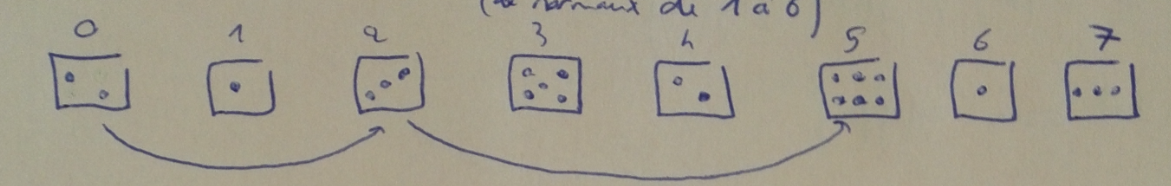
\includegraphics[width=.8\linewidth]{images/exo_2016_5}
\end{center}
À partir du premier dé on avance de $k$ dés avec $k$ la valeur du dé comme ci-dessus jusqu'à que ce ne soit plus possible.

\begin{enumerate}
\item Écrire une fonction \texttt{lancer} sans argument qui modélise un lancer de dé (la méthode \texttt{random} était donnée mais pas son fonctionnement). 
\item Écrire une fonction \texttt{liste} d'argument $n$ qui renvoie une liste de $n$ lancées de dés. 
\item Écrire une fonction \texttt{arrivee} d'argument $k$ et $L$ avec $k$ l'indice du premier dé pris en compte (dans l'exemple du haut $k=0$) et $L$ une liste de lancés de dés qui donne l'indice du dernier dé pris en compte. La tester pour tous les $k$ avec des listes de 15, 20 et 25 lancés. Que remarquez-vous ?
\item Écrire une fonction \texttt{commun} d'argument $L$, une liste de lancés qui renvoie le plus grand entier $k$ tel que l'indice d'arrivée en partant de 0, 1, 2, $k$ soit le même.
\end{enumerate}

\subsection*{Exercice 9}
Soit $f$ définie sur $[0,+\infty[$ tel que si $0\leq x< 1$, $f(x)=g(x)$, si $x>1$, $f(x)=xf(x-1)$. 

\begin{enumerate}
\item Avec $g(x)=1$, créer une fonction $H(x)$ qui est la continuité de $f(x)$ sur $]-1,0]$. 
\item Créer $f(x)$ entre $]-1,+\infty[$.
\item Tracer $f(x)$ entre $]-1,4y[$.
\item Tracer la dérivée de $f(x)$.
\item Même chose avec $g(x)=\cos x$.
\end{enumerate}

%Exercice 1
\subsection*{Exercice 10}
Pour le python c'était un sujet sur les mots et les bon mots.
\begin{enumerate}
\item Créer une fonction \textbf{mots(n)} qui retourne la listes des listes de longueur $n$
avec le nombre $1$ aux différents endroit possibles. \\
Par exemple pour une longueur 2: (0,1);(1,0) .
\item Un bon mot est une liste ou on a deux fois le nombre 1 consécutivement
à l'intérieur.
Écrire une fonction \textbf{bon\_mot(mot)} renvoyant un booléen qui détermine
 si la liste est un bon mot ou non
\end{enumerate}

%Exercice 4
\subsection*{Exercice 11}
\begin{enumerate}
\item Écrire une fonction pol(L,x) d'argument une liste $L=[a_n,..,a_0]$ des 
coefficients d'un polynômes $P$ et $x$ un flottant et renvoyant $P(x)$.
\item Définir la matrice $M$ donnée (4x4).
\item On définit la suite de matrice $B_0=M$ et relation de récurrence entre $B_k$
et $B_{k-1}$, écrire une fonction calculant la matrice $B_k$
\end{enumerate}


% 5
\subsection*{Exercice 12}
\begin{enumerate}
\item Écrire une fonction divise d'argument un entier $n$ et qui renvoie la liste de 
ses diviseurs de carré inférieur ou égal à $n$.
\item Écrire une fonction est\_premier d'argument un entier $n$ et qui renvoie le booléen 
correspondant correspondant à "n est premier".
\item Écrire une fonction nbp d'argument un entier $n$ et qui renvoie le nombre de
 nombre premiers entre $2$ et $n$.
 \item Deux autres non traitées.
 %P=x2-x-41 premiers 0 à 40 et x2-79x+1601 premiers de 0 à 79
\end{enumerate}

% Exo 6
\subsection*{Exercice 13}
On considère les fonctions suivantes : 
$$h(t)=\left\{
 \begin{array}{l} 
 1  \text{ si } t \in \mathbb{R}_{+}^{*} \\ 
 0  \text{ si } t\leq 0
\end{array}\right.
$$
et 
$\rho(t)=\sqrt{h(\cos(2t))\cos(2t)}$.\\
Et la courbe $\Gamma$ de représentation paramétrique 
$x(t)=\rho(t)\cos(t)$ et $y(t)=\rho(t)\sin(t)$.
\begin{enumerate}
\item Écrire la fonction \bf $\rho(t)$ \rm d'argument $t$
\item Écrire une fonction \bf pts \rm d'argument un entier naturel et qui renvoie la liste 
de couples des coordonnées $(x_i,y_i)$ des points $M(t_i)$ de $\Gamma$, pour 
$n+1$ valeurs de $t_i$ régulièrement réparties dans $[0,2\pi]$.
\item Tracer sur un même graphique les lignes polygonales approchant la courbe
 $\Gamma$ pour les valeurs $n=50$ et $n=1000$.
\item Écrire une fonction \bf longueur \rm d'argument une liste de couples de
 coordonnées et qui renvoie la longueur de la ligne brisée reliant les points de la liste.\\
 Calculer la longueur approchée de la courbe.
\end{enumerate}

%7
\subsection*{Exercice 14}
On définit la suite $(t_n)$ par $t_0=0$, $t_{2n}=t_n$ et $t_{2n+1}=1-t_n$
\begin{enumerate}
\item Définir  une fonction \bf t \rm d'argument un entier $n$, récursive et renvoyant 
$t_n$.\\
On appelle MOT T la chaine de caractère associée aux termes de $(t_n)$ : "0110100.."
\item Définir une fonction une fonction \bf mot \rm d'argument un entier naturel $n$ 
et qui renvoie les $n$ premiers caractère de MOT T. 
\item Définir \bf nbseq \rm d'arguments un entier $n$ et une chaine de 
caractères seq, renvoyant le nombre d'apparitions de la chaine seq dans le mot mot(n).
\item Conjecturer la limite de $\frac{nbseq(n,seq)}{n}$  pour des séquences à
$1$, $2$ ou $3$ bits.
\item ....
\end{enumerate}

%8
\subsection*{Exercice 15}
Données fournies : décimales de $\pi$ dans un fichier texte
\begin{enumerate}
\item Ouvrir le fichier et récupérer les donnes sous forme d'une chaine de caractères.
\item Afficher les dix premières décimales, les 10 dernières du fichier, 
le nombre de décimales.
\item Écrire une fonction \bf tirer \rm d'arguments un entier $n$ , $C$ (chaine de
 longueur $N$) et $p$ (dans $[1,N]$), renvoyant une liste de longueur $n$ de chiffres 
compris entre $0$ et $9$ d'éléments ressortant de la lecture de $C$ entre 
$C[p]$ et $C[p+n-1]$. (si on arrive à la fin de $C$ on recommence au début)
\end{enumerate}

% 11
\subsection*{Exercice 16}
\begin{enumerate}
 \item Écrire une fonction bin(d) d'argument un entier $d$ non nul et renvoyant 
 le nombre de  chiffres dans l'écriture binaire de $d$.
 \item Écrire la fonction f(a) retournant $a^{n+1}-2^{n+1}$ où $n$ est le nombre de chiffres dans l'écriture binaire de $a$ (?)
% Peut- être $a-2^n$ ? si $n\geq 1$ et $0$ sinon
\item Écrire une fonction créant la liste de $n$ éléments utilisant la fonction 
$f$ telle que $u_{n+1}=f(u_n)$. % A voir
\item ?\\
%Ecrire une fonction retournant le nombre de un dans l'écriture binaire d'un entier.
 \end{enumerate}


%12 
\subsection*{Exercice 17}
\begin{enumerate}
\item Écrire une fonction d'argument $n$ et renvoyant une liste de toutes listes de longueurs $n$ possibles, formées de $1$ et de $-1$.\\
Pour $n=2$ la fonction doit renvoyée $[[1,1],[1,-1],[-1,1],[-1,-1]]$.
\item ?
\item ?
\end{enumerate}

%13
\subsection*{Exercice 18}
\begin{enumerate}
\item Écrire une fonction d'argument  un entier $n$ et renvoyant le nombre "inversé"
$1234$ devient $4321$.
\item Écrire une fonction d'argument un entier et retournant le booléen représentant 
"n est un palindrome".
\item Créer une fonction d'argument $n$ et renvoyant la liste des entiers de $0$ à 
$n$ identiques à leur palindrome.
\item Reprendre la question 1 en écrivant une fonction récursive.
\end{enumerate}

%14
\subsection*{Exercice 19}
Un enfant a deux boites de bonbons (une dans chaque poche) contenant 
$N_a$ et $N_b$ bonbons. Il tire au hasard une des deux boites; si elle est vide 
il s'arrête de manger des bonbons, sinon il prend un bonbon et remet la boite dans 
sa poche, puis recommence.
\begin{enumerate}
\item Écrire une fonction donnant le nombre de bonbons mangés.\\
Utiliser le module rand de numpy.
\item Estimer la loi de probabilité définissant le nombre de bonbons mangés et 
quelle boite sera vide sur $n$ expériences.
%Pas très clair à voir
\end{enumerate}

\subsection*{Exercice 20}
Un jeu de carte est composée de $32$ cartes, une carte est un couple $[valeur,couleur]$
où $valeur$ appartient à $valeurs=["7","8","9","10","V","D","R","A"]$
et $couleur$ appartient à $couleurss=["trefle","coeur","carreau","pique"]$
\begin{enumerate}
 \item Représenter le jeu de carte dans une liste.
 \item Définir une fonction sans argument tirermain() qui retourne une liste de $5$ cartes au hasard. On pourra utiliser la fonction sample du module random.
 (l'examinatrice m'a orienté vers randint)
\item Définir une fonction LV d'argument une main et qui retourne une liste du nombre de fois qu'apparait chaque valeur dans la main, dans l'ordre croissant, pour une paire 
la fonction retourne $[1,1,1,2]$.
\item ?
\item ?
\item Estimer la probabilité d'obtenir une paire, un brelan, un carré.
 \end{enumerate}
\end{multicols}

\newpage 
\section{Exercices de la Banque PT -- 2016 -- à vérifier }
\begin{multicols}{2}

%


\subsection*{Exercice 1}
\begin{enumerate}
 \item Compréhension d'un programme qui stocke dans deux listes les quotients et restes
 de la division par $4$
 \item Une liste de réels était donnée avec $16$ éléments $L=[.,....,.]$
 Il fallait la découper en paquets de 4 $L=[[...],[...]...]$, puis la transformer en chaine de 
 caractère $m=... ch(16a_0+64a_1+?a_2+?a_3)$.\\
 Cette chaine renvoyait le mot OK.\\
 %Codage ? ecriture en base 4 ?
 \end{enumerate}
 



%
%%
%\end{multicols}
%
%\newpage 
%\begin{multicols}{2}
%\section{Exercices de la Banque PT -- 2016}
%\addcontentsline{toc}{subsection}{Exercice 1}
\subsection*{Exercice 2}

\begin{enumerate}
\item Écrire une fonction $P$ d'argument $L$ telle que $L = [l_0, l_1,…,l_{d-1}]$ et $C = [c_0,c_1,…,c_{d-1}]$ (deux listes) qui renvoie le produit du vecteur ligne par le vecteur colonne
\item Soit $M$ une matrice carré sous forme d'une seule ligne (exemple : $M = [m_0,m_1,m_2,m_3]$ est une matrice 2x2 $\begin{pmatrix} m_0 & m_1 \\m_2 & m_3 \end{pmatrix}$. Écrire une fonction d'argument $M$ une matrice carrée sous forme d'une liste, et un entier $i$ qui renvoie la ligne $i$ de la matrice $M$.
\item Écrire une fonction d’argument $M$ et $j$ qui renvoie la colonne $j$ de la matrice $M$ (toujours une matrice sous forme d'une liste).
\item Écrire une fonction d'argument $M$ et $N$, deux matrices carrées sous forme d'une liste, et qui renvoie le produit matricielle de $M$ par $N$. 
\end{enumerate}


%
%Un pays ne produit que des billets de 57 62 et 72 unités.
%\begin{enumerate}
%\item Peut-on atteindre les sommes de 400 et 600 avec ces billets ?
%\item Écrire la fonction comptage qui permet de dire si une somme est décomposable en billets et de combien de manière différentes. 
%\item Un enfant achète un croissant qui coûte 4 unités il utilise deux valeurs de billets le boulanger lui rend que des billets combien l'enfant a-t-il donné au boulanger (le détail) ?
%\end{enumerate}



%%\addcontentsline{toc}{subsection}{Exercice 2}
%\subsection*{Exercice 2}
%
%On donnait un programme (utilisant des nombres complexes, \texttt{numpy} et \texttt{numpy.rand}).
%\begin{enumerate}
%\item Que fait ce programme ? (Il donnait une liste de complexes de parties réelles aléatoires, centrées autour de 50, et de partie imaginaires aléatoires centrées autour de 20). Représenter sa sortie (un nuage de point).
%\item  Écrire une fonction bornes d'argument une liste de complexes \texttt{L} donnant les abscisses et ordonnées maximales des éléments de \texttt{L} dans le plan complexe
%\item  Tracer le rectangle basé sur les points obtenus par la fonction précédente à partir des points donnés par le programme donné.
%\item  On souhaite minimiser l'aire du rectangle encadrant le nuage de points. Pour cela on va écrire un programme d'argument une liste de complexes \texttt{L} et un entier \texttt{n}.
%On va procéder à des rotations d'angle $-a$ du repère, pour $a$ entre 0 inclus et $2\pi$ exclus, avec un pas de $\dfrac{2\pi}{n}$. À chaque étape on trace le rectangle qui colle au mieux, puis on garde celui d'aire minimale. Ensuite, tracer ce rectangle.
%\item La même question mais en traçant un rectangle (je ne l'ai pas faite).
%\end{enumerate}


%\addcontentsline{toc}{subsection}{Exercice 3}
%\subsection*{Exercice 3}





%\addcontentsline{toc}{subsection}{Exercice 4}
\subsection*{Exercice 3}
On a : $\mathcal{P}_1$, $\mathcal{P}_2$, ..., $\mathcal{P}_n$ populations d'un grand nombre d'individus. $\mathcal{P}_i  =\dfrac{i}{n}$ la population vérifiant $\mathcal{C}$. On choisit $n$ individus et on note $X$ le nombre d'individus vérifiant $\mathcal{C}$.
\begin{enumerate}
\item Sachant $\mathcal{P}_i$, calculer $P\left(X=h\right)$.
\item Définir la fonction \texttt{tirer} qui simule cela en utilisant \texttt{randint}. 
\end{enumerate}

%\addcontentsline{toc}{subsection}{Exercice 5}

%\addcontentsline{toc}{subsection}{Exercice 6}
\subsection*{Exercice 4}

\begin{enumerate}
\item Faire une fonction <<partage>> d'arguments \texttt{L} une liste de chiffre et \texttt{a} un chiffre, elle devrait renvoyer deux liste \texttt{Linf} qui correspond a la liste des élément de \texttt{L} inférieur ou égale à \texttt{a} et \texttt{Lsup} (réciproquement).
\item Faire une fonction \texttt{tri\_rapide} à l'aide de la fonction \texttt{partage}.
\item Modifier tri pour quelle renvoie le nombre de comparaison (je n'ai pas réussi à modifier la récurrence pour obtenir les comparaisons).
\item Essayer la fonction avec une liste de 1000 éléments aléatoires, compris entre -999 et 999.
\end{enumerate}


%\addcontentsline{toc}{subsection}{Exercice 7}
%\addcontentsline{toc}{subsection}{Exercice 8}
\subsection*{Exercice 5}

Un physicien réalise une expérience et stocke les données dans un fichier. Il y a 41 positions (de -20 à 20) et deux points extrêmes désignant la frontière de l’étude (-25 et 25), soit 43 points au total. Les résultats sont des probabilités de présence autour des points. Il souhaite déterminer le modèle le plus adéquat.
Le fichier est enregistré sous la forme :  

\texttt{2500}\\

\texttt{2.56}

\texttt{6.89}

...

Avec le premier nombre désignant le nombre de valeurs puis la liste des probabilités de présence pour chaque point.
\begin{enumerate}
\item Écrire la fonction \texttt{nomfic} de paramètre $n$ (un entier compris entre 0 et 99) retournant la chaîne de caractère \texttt{`data/modele152-xy.txt'} avec $x$ le nombre des dizaines et $y$ le nombre des unités. (Ex : \texttt{nomfic(7) -> ‘data/ modele152-07.txt’}).

\item Écrire la fonction \texttt{ecart} de paramètres $F$ et $P$ (deux listes contenant des probabilités de présence) et qui renvoie : $E=\sum\limits_{i=0}^{n}\dfrac{f_i-p_i}{p_i}$.


\item Lire le fichier \texttt{‘data/experience152.txt’} dans le format détaillé précédemment avec $N$ le nombre de valeurs et $F$ la liste de probabilités.
Vérifier que la somme des probabilités vaut 1.
Afficher le nuage de point des probabilités en fonction de la position.
\item Parcourir tous les fichiers de modèle (de la même forme que l’expérience mais sans le nombre de valeurs) et pour chaque ?? :
\begin{enumerate}
\item extraire $P$ la liste des probas;
\item trouver le minimum de $P$ : $N_{min}$;
\item si $N>N_{min}$ : $E=N\cdot \text{ecart}(F,P)$.
\end{enumerate}
\end{enumerate}

Et je ne me souviens plus tout à fait de la suite, il faut certainement récupérer le modèle correspondant à l’écart le plus faible et le tracer sur la courbe précédente.


%\addcontentsline{toc}{subsection}{Exercice 9}
%\addcontentsline{toc}{subsection}{Exercice 10}

%
%
%\addcontentsline{toc}{subsection}{Exercice 11}


%\addcontentsline{toc}{subsection}{Exercice 12}
%\subsection*{Exercice 12}


\end{multicols}

\newpage 
\begin{multicols}{2}
\section{Exercices de la Banque PT -- 2015 -- \ding{51}}
%\addcontentsline{toc}{subsection}{Exercice 7}
\subsection*{Exercice 1}
<< Il m'était demandé de créer une liste regroupant les abscisses et ordonnées pour $k$ allant de 1 à 12, des points complexes de module variant entre 0 et 1, d'angle $\dfrac{k\pi}{6}$ et ensuite de tracer ces points. Je suis arrivé à le faire mais j'ai été obligé de me faire confirmer par l'examinateur ce qu'il fallait faire car l'énoncé me bloquait.
>>

Précision sur l'énoncé : tracer dans le plan complexe des points de module
$k/12$ et d'argument $k\cdot pi/6$, $k$ entre 0 et 12.

%\addcontentsline{toc}{subsection}{Exercice 8}
\subsection*{Exercice 2}
\begin{rem}
Exercice tombé au moins deux fois.
\end{rem}

Un segment $[a,b]$ est noté comme une liste \texttt{[a,b]}. Soient $I_1$ et $I_2$ deux segments. Ils sont disjoints si leur intersection est vide. 

\begin{enumerate}
\item Écrire une fonction \texttt{disjoint} d'arguments $i_1$ et $i_2$ (deux listes représentant des segments) et retournant \texttt{True} s'ils sont disjoints, \texttt{False} sinon. 
\item La fusion de deux segments correspond à un segment qui a pour min le plus petit des deux min et pour max le plus grand des deux max. Écrire une fonction \texttt{fusion} d'arguments $i_1$ et $i_2$ et qui retourne la liste correspondant à la fusion de ces deux segments. 
\item On dit qu'une liste de segments est bien fondée si les segments de cette liste sont disjoints et rangés dans l'ordre croissant. (On dit que $I_1=[a,b]$ est inférieur à $I_2=[c,d]$ si $b<c$.)
\begin{enumerate}
\item Les listes suivantes sont-elles bien fondées : $L=[[0,3],[6,7],[2,5]]$ et $L=[[0,1],[2,3],[4,5]]$ ?
\item Écrire une fonction récursive \texttt{verif} qui dit si une liste est bien fondée ou non.
\end{enumerate}
\end{enumerate}



%\addcontentsline{toc}{subsection}{Exercice 9}
\subsection*{Exercice 3}
Voici un théorème d'arithmétique : tous les nombres entiers sont au plus décomposables en une somme de 9 cubes. 
\begin{enumerate}
\item Définir une fonction \texttt{estcube(n)} qui retourne \texttt{True} si $n$ est un cube, \texttt{False} sinon. Afficher tous les cubes inférieurs ou égaux à 250.
\item Définir une fonction \texttt{S2cube(n)} qui retourne \texttt{True} si $n$ est la somme de deux cubes, \texttt{False} sinon. Afficher tous les entiers inférieurs ou égaux à 250 qui sont somme de deux cubes.
\item Définir une fonction \texttt{S4cube(n)} qui retourne \texttt{True} si $n$ est la somme de quatre cubes, \texttt{False} sinon. Afficher tous les entiers inférieurs ou égaux à 250 qui ne sont pas somme de deux cubes.
\item Définir une fonction \texttt{S8cube(n)} qui retourne \texttt{True} si $n$ est la somme de huit cubes, \texttt{False} sinon. Afficher tous les entiers inférieurs ou égaux à 250 qui ne sont pas somme de deux cubes.
\item Expliquer pourquoi les nombres qui ne sont pas somme de 8 cubes sont sommes de 9 cubes. 
\item Conclure.
\end{enumerate}


\end{multicols}


\newpage 
\begin{multicols}{2}


\section{Exercices de la banque PT retranscrits par vos prédécesseurs -- 2015}
\begin{rem}
Les exercices vous sont retranscrits tels que vos prédécesseurs nous les ont retranscrits. 
\end{rem}
%%\addcontentsline{toc}{subsection}{Exercice 1}
%\subsection*{Exercice 1}
%Nombre de manières de payer $n$ euros avec des pièces de \texttt{L} (liste de valeurs).  
%
%%\addcontentsline{toc}{subsection}{Exercice 2}
%\subsection*{Exercice 2 -- Nombres riches ?}
%Écrire une fonction qui donne les diviseurs d'un entier $n$, puis qui donne les $k$ premiers nombres riches et leur nombre de diviseurs sous forme d'une liste contenant des groupes comme \texttt{[2,2]} ? Question sur les facteurs premiers.
%
%%\addcontentsline{toc}{subsection}{Exercice 3}
%\subsection*{Exercice 3}
%<< C'était une histoire de n listes de taille n dans une liste et je devais construire par récursivité un programme qui me donnait le nombre maximal de listes possibles de taille \texttt{p} dans ma liste de liste.>>


%\addcontentsline{toc}{subsection}{Exercice 4}
\subsection*{Exercice 4}
On considère la somme $S=\sum\limits_{n=1}^{+\infty} \dfrac{(-1)^n}{n}$.
\begin{enumerate}
\item Montrer que le reste de la série vérifie $\left| R_n \right| \leq \dfrac{1}{1+n}$.
\item Écrire une fonction qui calcule la somme $S$ à $10^{-6}$ près.
\item Tracer $S_n$ en fonction de $n$ (on rendra une centaine de points).
\end{enumerate}

%\addcontentsline{toc}{subsection}{Exercice 5}
\subsection*{Exercice 5}
Dans un ensemble $E=\left\{ a_1, a_2, ..., a_n\right\}$, $A_i$ représente une partie de  $E$ et est représenté par le code $c_i$ tel que $c_i[k]=0$ si $a_k \in A_i$ et 1 sinon.
\begin{enumerate}
\item Écrire la fonction \texttt{reunion} d'arguments $c_1$ et $c_2$ codes respectifs de $A_1$ et $A_2$ et retournant le code de $A_1 \bigcup A_2$. 
\item Écrire la fonction \texttt{estrec} d'argument \texttt{L} une liste de codes associés à des sous ensembles de $E$ et retournant le booléen \texttt{True} su la réunion de ces sous ensembles vaut \texttt{E} ou \texttt{False} sinon.
\item Soit $R$ un ensemble de parties de $E$ représenté par une liste $L$ de codes. On dit que $R$ est un recouvrement minimal de $E$ si la réunion des parties de $R$ est $E$ et que pour tout $R'$ inclus dans $R$ et différent de $R$, $R'$ n'est pas un recouvrement de $E$ (la réunion des parties de $R'$ est différente de $E$. 
\item Écrire la fonction \texttt{estRecMin} d'argument \texttt{L} une liste de codes représentant $R$, qui retourne le booléen \texttt{True} si $R$ est un recouvrement minimal de $E$ \texttt{False} sinon. 
\end{enumerate}

%\addcontentsline{toc}{subsection}{Exercice 6}
\subsection*{Exercice 6}
Soit $s$ définie par $s_0=1$,  $s_1=1$, et pour tout $n$, $s_{2n}s_n+s_{n+1}$. 
\begin{enumerate}
\item Calculer les 8 premiers termes de la suite.
\item Écrire la fonction \texttt{LS} d'argument $N$ et renvoyant les $N+1$ premiers éléments de la suite $s$. Calculer $L_{128}=LS(128)$. 
\item On sépare la liste $L_{128}$ de 1 à 2, de 2 à 4, de 4 à 8... Quelle symétrie y a-t-il pour chaque paquet ? Extraire ces paquets.
\item Écrire la fonction \texttt{LP} d'argument $N$ et renvoyant les $N+1$ premières lignes du triangle de Pascal. On rappelle que $\begin{pmatrix}n+1 \\ p \end{pmatrix}=\begin{pmatrix}n \\ p-1 \end{pmatrix}+\begin{pmatrix}n \\ p \end{pmatrix}$ et $\begin{pmatrix}n \\ 0 \end{pmatrix} = \begin{pmatrix}n \\ n \end{pmatrix}=1$.
On a par exemple, $TP(4)=[[1],[1,1],[1,2,1],[1,3,3,1],[1,4,6,4,1]$.
\item ...
\end{enumerate} 







%\addcontentsline{toc}{subsection}{Exercice 10}
\subsection*{Exercice 10}
On dit qu'un mot est un palindrome s'il est le même lorsqu'on le dit à l'envers. Par exemple le mot <<radar>> est un palindrome. Le mot <<nul>> donne <<lun>> à l'nvers et n'est pas un palindrome. 
\begin{enumerate}
\item Écrire une fonction \texttt{inverse} d'argument une chaine de caractères \texttt{mot} et renvoyant la chaîne écrite à l'envers. 
\item Écrire une fonction \texttt{palindrome} d'argument une chaine de caractères \texttt{mot} et renvoyant le booléen \texttt{True} si le mot est un palindrome, \texttt{False} sinon.
\item Par extension on dit qu'un nombre est un palindrome s'il est égal au nombre obtenu en écrivant les chiffres en ordre inverse. Écrire une fonction \texttt{pat\_nombre} d'argument $N$ et renvoyant la liste des nombres palindromes inférieurs ou égaux à $N$.
\end{enumerate}


%\addcontentsline{toc}{subsection}{Exercice 11}
\subsection*{Exercice 11}
\begin{enumerate}
\item Créer une fonction \texttt{partage} prenant en argument une liste $L$ et un entier $a$ retournant 2 listes $Linf$ et $Lsup$ respectivement les listes des éléments de $L$ inférieurs à $a$ et et ceux supérieurs à $a$.
\item Créer une fonction \texttt{trirapide} utilisant la précédente. 
\item Modifier les deux fonctions précédentes afin de connaître le nombre de comparaisons effectuées. 
\item Tester votre fonction avec une liste de 4000 valeurs entre -999 et 999. Utiliser \texttt{randint(p,q)} pour créer cette liste.
\end{enumerate}

%\addcontentsline{toc}{subsection}{Exercice 12}
\subsection*{Exercice 12}
On qualifie un vecteur de creux lorsque le nombre de zéros qu'il contient est au moins supérieur à la moitié de son nombre de coordonnées. Par exemple $v=\left(1,2,0,4,7,0,0,0,0\right)$ est creux (5 zéros et 9 coordonnées). Son codage est creux est $v=\left[9,[1,2,4,7],[0,1,3,4]\right]$ (nombre de coordonnées, liste des éléments non nuls, liste des indices de ces éléments).
\begin{enumerate}
\item Définir la fonction \texttt{creux} d'argument une liste $v$ représentant un vecteur et retournant un booléen indiquant si le vecteur est creux ou non.
\item Définir la fonction \texttt{coder} d'argument une liste $v$ représentant un vecteur et retournant le codage creux du vecteur.
\item Définir une fonction \texttt{decoder}.
\item Définir une fonction \texttt{simul} d'argument le codage \texttt{C} d'un vecteur $v$ et un scalaire $a$ retournant le cordage creux du vecteur $av$.
\item Définir une fonction \texttt{coefficient(j,C)} qui renvoie la coordonnée $j$ du vecteur creux associé au code $C$.
\end{enumerate}

%\addcontentsline{toc}{subsection}{Exercice 13}
\subsection*{Exercice 13}
\begin{enumerate}
\item Créer une fonction $\texttt{C}$ d'argument un entier $d$ et qui renvoie un entier formé par les chiffres de $d$ dans l'ordre croissant. Par exemple, $C(1542)=1245$.
\item Créer une fonction $\texttt{D}$ qui fait la même chose que $\texttt{C}$ mais dans l'ordre décroissant. 
\item On définit une suite $u_n$ par $u_0=a \in \mathbb{N}$ et $u_{n+1}=D(u_n)-C(u_n)$. Écrire une fonction qui calcule les termes de cette suite.
\item ...
\end{enumerate}

%\addcontentsline{toc}{subsection}{Exercice 14}
\subsection*{Exercice 14}
\begin{enumerate}
\item Créer une fonction \texttt{nbits} d'argument un entier \texttt{n} qui renvoie le plus petit entier $i$ tel que $n \leq 2^i$. 
\item Créer une fonction \texttt{sansrep} d'argument une liste $L$ d'entiers et qui retourne la liste des éléments de $L$ en unique exemplaire. Exemple : \texttt{sansrep([5,0,0,0,3,3,5])=[5,0,5]}. On utilisera la fonction \texttt{in}.
\item Créer une fonction \texttt{position} d'argument une liste $L$ d'entiers et $e$ un entier, retournant la première position de $e$ dans $L$ (en supposant que $e$ est dans $L$).
\item Retourner l'écriture binaire de la position de $e$ dans la liste. On utilisera \texttt{nb.format(i)}.

\end{enumerate}

%\addcontentsline{toc}{subsection}{Exercice 15}
\subsection*{Exercice 15}
Soit $n$ un entier fixé. On étudie le codage de listes d'entiers de longueur.  On dispose d'une liste représentant le codage $\texttt{C}$ de longueur $n$ contenant des 0 et des 1.  Une liste $\texttt{E}$ d'entiers de longueurs $n$ est la liste codée d'une liste $A$ telle que $A$ contient les éléments de la liste $E$ dont les indices sont ceux pour lesquels $\texttt{C}$ contient 1. 
Ainsi si \texttt{E=[2,4,6,7]} et \texttt{C=[0,1,1,0]} alors \texttt{A=[4,6]}.
\begin{enumerate}
\item Créer une fonction \texttt{decoder} d'arguments deux listes \texttt{E} et \texttt{C} qui renvoie la liste \texttt{A}.
\item Créer une fonction \texttt{coder} d'arguments \texttt{E} et \texttt{A} retournant \texttt{C}.
\item Créer une fonction \texttt{incrementer} d'argument \texttt{C} et retournant une liste \texttt{C'} contenant l'écriture binaire du nombre $N+1$ avec $N$ nombres dont l'écriture binaire est $C$ (si \texttt{C=[0,1,1,0]}, \texttt{N=6} donc \texttt{N+1=7} et \texttt{C'=[0,1,1,1]}.
\end{enumerate}


%%\addcontentsline{toc}{subsection}{Exercice 15}
%\subsection*{Exercice 15}
%\textit{NDLR : Je ne sais pas si c'était un exo de maths ou de Python.}
%<< J'ai eu un exercice de proba: 
%un ordinateur et deux réseau dont le choix est indépendant 
%on choisi a 70\% le $A$ et proba d'avoir une erreur avec $A$ $e=0,1$ avec $B$ $e=0.05$.
%\begin{enumerate}
%\item Calculer la proba d'avoir une erreur.
%\item On a une erreur. Calculer la proba d'avoir choisi A. \\
%
%On considère une liste par exemple AAAABBA..., L1 liste d'avoir 4 fois le réseau A, L2, 2fois le réseau B.
%
%\item Montrer que la série des L1 (pour $k\geq 1$) est égale à 1.
%\item L1 admet-elle une espérance ? Si oui la calculer.
%\item Calculer la proba de (L1,L2).
%\item ???
%\end{enumerate}

%\addcontentsline{toc}{subsection}{Exercice 15}
\subsection*{Exercice 15}
Soit $T_n$, le reste de la division euclidienne par 2 de la somme des chiffres représentant $n$ en base 2.
(exemple : 13 s'écrit 1101 donc on regarde le reste de la division de 1+1+0+1 par 2, donc $T(13)=1$). 

\begin{enumerate} 
\item \begin{enumerate}
\item Trouver une relation entre $T_{2n}$ et $T_n$.
\item De-même, trouver une relation entre $T_{2n+1}$ et $T_n$.
\item Créer une fonction récursive pour calculer $T_n$
\end{enumerate}
\item Afficher les lignes suivantes: 
\begin{itemize}
\item $T_0$, $T_1$
\item $T_0$  $T_1$ ; $T_2$ $T_3$;
\item $T_0$ $T_1$ $T_2$    ; $T_3$ $T_4$ $T_5$.
\end{itemize} 
Remarquer une particularité et en déduire une manière simple de calculer les $2^p$ premiers termes de la suite $T_n$.
\item Montrer que : $\sum\limits_{n=0}^{+\infty} = \dfrac{T_n}{2^{n+1}}$ converge.
\item Calculer numériquement une valeur approchée de la somme à $10^(-6)$ près.
\end{enumerate}

%\addcontentsline{toc}{subsection}{Exercice 16}
\subsection*{Exercice 16}
\begin{enumerate}
\item Créer une fonction qui compte le nombre d'éléments pairs d'une liste. 
\item Créer une fonction qui crée la liste des éléments pairs d'une liste. 
\item Créer une fonction qui renvoie le booléen \texttt{True} si la liste ne contient que des chiffres pairs, \texttt{False} sinon. 
\item Créer une fonction qui donne la position du maximum dans la liste. 
\item Créer une fonction qui donne la médiane de la liste. 
\item Créer une liste de 20 nombres aléatoires entre 0 et 100. Tester les fonctions. 
\end{enumerate}

%\addcontentsline{toc}{subsection}{Exercice 17}
\subsection*{Exercice 17}
\begin{enumerate}
\item Écrire une fonction \texttt{binaire} d'argument $n\in\mathbb{n}$, renvoyant sous forme de liste l'écriture binaire de $n$/
\item Écrire une fonction \texttt{nombreDeUn} d'argument $n\in \mathbb{N}$, renvoyant le nombre de 1 dans \texttt{binaire(n)}. 
\item La définition du <<n-palindrome>> était donnée dans l'énoncé.
\begin{enumerate}
\item Écrire une fonction \texttt{Palindrome} d'argument $n\in \mathbb{N}$ permettant de déterminer si n est un 2-palindrome.
\item Donner les 2-palindromes entre 0 et 100.
\end{enumerate}
\end{enumerate}



%\addcontentsline{toc}{subsection}{Exercice 18}
\subsection*{Exercice 18}
Les nombres sont écrits sous forme de chaîne de caractères.
\begin{enumerate}
\item Déterminer tous les entiers inférieurs à 10000 égaux à la puissance 4 de la somme de leurs chiffres.
\item Écrire une fonction \texttt{DixVersDeux} qui prend comme argument un nombre en base 10 (chaine de caractères) et envoie le nombre en base 2. 
\item Écrire une fonction \texttt{DeuxVersDix} réciproque de la fonction précédente. 
\item Déterminer tous les entiers inférieurs à 10 000 égaux à la puissance 4 de la somme de leurs chiffres en base 2.
\item Écrire une fonction  \texttt{DixVersBase(chaine,base)}. 
\item Refaire la question 4 avec les bases 3 à 9.
\end{enumerate}

%\addcontentsline{toc}{subsection}{Exercice 18 -- Bis}
\subsection*{Exercice 18 -- Bis}
On écrit 18 par une chaine de caractères : \texttt{'18'} en base 10 et \texttt{'10010'} en base 2. 
\begin{enumerate}
\item Écrire une fonction \texttt{somchi} d'argument une chaine de caractères et retournant la somme de ses chiffres  (exemple \texttt{somchi('18')} retourne 9).
\item Donner la liste des nombres entiers égaux à la somme de leurs chiffres à la puissance 4. 
\item Écrire la fonction \texttt{DixVersDeux}, d'argument une chaine de caractère d'un nombre en en base 10 et retournant le nombre en base 2. 
\item Écrire la fonction réciproque \texttt{DeuxVersDix}.
\item Donner la liste des nombres entiers en base 2 égaux à la puissance 4 de la somme de leur chiffre.
\end{enumerate}


%\addcontentsline{toc}{subsection}{Exercice 19}
\subsection*{Exercice 19}

\begin{itemize}
\item Deux algorithmes à expliquer (l'un transforme un nombre en une liste de ses chiffres et l’autre est la fonction inverse) exemple : 2015 : alg1 $\rightarrow$  [2, 0, 1, 5] --  alg2  $\rightarrow$ 2015.
\item Écrire la fonction récursive \texttt{perm} d’argument une liste \texttt{L} qui renvoi toute les permutations
de cette liste.
\item 2 autres questions non traitées.
\end{itemize}

%\addcontentsline{toc}{subsection}{Exercice 20}
\subsection*{Exercice 20}
Soit $x$ un réel, $v_0=x$, $a_n = \lfloor v_n \rfloor$, $v_{n+1} = \left\{ \begin{array}{l} 0 \\ \dfrac{1}{a_n -1} \end{array} \right.$ si $a_n>1$.
\begin{enumerate}
\item Calculer les 10 premiers termes de la suite pour $x=\sqrt{3}$. 
\item Définir $A(x)$, la fonction qui définit la suite et renvoie les 10 premiers termes de la suite. La tester avec $\sqrt{2}$, $\dfrac{1+\sqrt{5}}{2}$, $\sqrt{5}$. 
\item Définir la fonction $Nb(x)$ qui renvoie le numérateur et le dénominateur de $a+\dfrac{b}{n}$. 
\item Définir le quotient de la fonction $Q(x)$ qui renvoie le quotient $a_0+\dfrac{1}{a_1+\dfrac{1}{a_2+\dfrac{1}{a_3+...\dfrac{1}{a_r}}}}$ avec $r$ le plus petit entier tel que $a_r<1$.
\end{enumerate}


%\addcontentsline{toc}{subsection}{Exercice 21}
\subsection*{Exercice 21}
\begin{center}
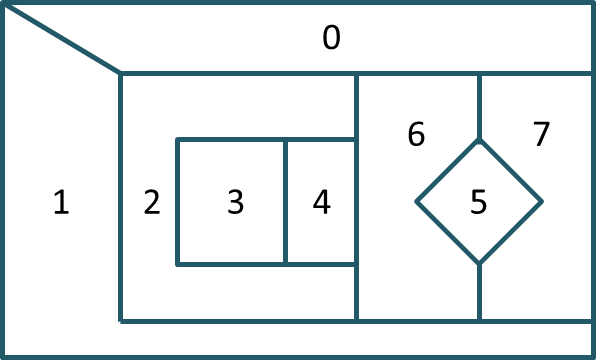
\includegraphics[width=.8\linewidth]{images/exo_21_pt_el.png}
\end{center}
Une carte numérotant des pays est numérotée de 0 à $i$.  Chaque pays se voit attribuer une couleur. Le but est que des pays voisins n'aient pas la même couleur. 

\begin{enumerate}
\item Écrire la liste carte constituée elle-même de liste donnant pour chaque pays le numéro des pays dont le numéro est supérieur à ce pays et ayant une frontière commune avec ce pays. Exemple : \texttt{carte[4]=[6]}, \texttt{carte[5]=[6,7]}.
\item Définir une fonction \texttt{voisins} de paramètres \texttt{(i,j,carte)} avec $i\neq j$. Cette fonction doit renvoyer un booléen \texttt{True} ou \texttt{False} si les pays $i$ et $j$ ont une frontière commune.
\item On attribue une couleur à chaque pays. Les couleurs sont représentées par des entiers naturels. On définit la liste \texttt{color} qui attribue pour chaque pays un numéro correspondant à sa couleur. Si le pays n'a pas de couleur, son numéro est $-1$. 

Définir la fonction \texttt{donnecouleur} de paramètre \texttt{p} pour le numéro de pays, \texttt{carte} et \texttt{color}. La fonction doit changer la liste couleur de façon à attribuer au pays \texttt{p} la couleur la plus petite tel qu'il ait une couleur différente de ses voisins. 

Exemple avec 3 : le pays 3 correspond à \texttt{p=2}. Admettons que les pays 2 et 4 aient respectivement les couleurs 1 et 2, on attribue à 4 la couleur 2. 
\end{enumerate}

%\addcontentsline{toc}{subsection}{Exercice 22}
\subsection*{Exercice 22}
Soit \texttt{L} une liste triée et \texttt{a} un réel. 
\begin{enumerate}
\item Écrire la fonction \texttt{ajout(L,a)} qui insère \texttt{a} dans \texttt{L} au bon endroit. 
\item Écrire la fonction \texttt{fusion(L1,L2)} qui classe en une liste triée la somme de \texttt{L1} et \texttt{L2}.
\end{enumerate}



%\addcontentsline{toc}{subsection}{Exercice 23}
\subsection*{Exercice 23}
On étudie les entiers tels que $n=a^3+b^3$. 
\begin{enumerate}
\item Montrer que $3$ ne s'écrit pas comme la somme de 2 cubes.
\item Écrire un programme afin de déterminer la liste des entiers $n$ tels que $n=a^3+b^3$ avec $n<100$.
\item Écrire une fonction renvoyant un booléen nous indiquant si $n$ est la somme de deux cubes. 
\item Écrire une fonction qui indique si $n$ est la somme de 2 cubes et l'ensemble des couples \texttt{(a,b)} tels que $n=a^3+b^3$.
\end{enumerate}

\end{multicols}


\newpage 


\begin{multicols}{2}

\section{Exercices issus de <<L'informatique pas à pas en prépa, éditions ellipses>>, Frédéric Butin}

%\addcontentsline{toc}{subsection}{Exercice 1 -- Opérations sur les polynômes}
\subsection*{Exercice 1 -- Opérations sur les polynômes -- 2.11.3 p.50}
\begin{flushright}
\textit{D'après Frédéric Butin, l'informatique pas à pas en prépa, éditions ellipses.}
\end{flushright}
Un polynôme $P=\sum\limits_{j=0}^{n}a_j X^j \in \mathbb{R}[X]$ de degré $n$ est représenté dans cet exercice par le tableau $P=[a_0,...,a_n]$.

\begin{enumerate}
\item Créer une fonction \texttt{affiche\_poly} qui permet d'afficher un polynôme sous la forme $P=\sum\limits_{j=0}^{n}a_j X^j$.
\item Créer une fonction \texttt{degre\_poly} qui calcule le degré d'un polynôme.
\item Implémenter la somme, le produit et la multiplication par un scalaire comme des fonctions notées \texttt{add\_poly}, \texttt{mul\_poly} et \texttt{mul\_sca\_poly}.
\item Créer une fonction \texttt{prsc\_poly} qui calcule le prduit scalaire canonique de deux polynômes.
\item Créer une fonction \texttt{deriv\_poly} qui calcule la dérivée d'un polynôme.
\end{enumerate}

%\addcontentsline{toc}{subsection}{Exercice 2 -- Produits polynômes}
\subsection*{Exercice 2 -- Produits polynômes -- 2.11.20 p.65}
\begin{flushright}
\textit{D'après Frédéric Butin, l'informatique pas à pas en prépa, éditions ellipses.}
\end{flushright}
Un polynôme $P=\sum\limits_{j=0}^{n}a_j X^j \in \mathbb{R}[X]$ de degré $n$ est représenté dans cet exercice par le tableau $P=[a_0,...,a_n]$.

\begin{enumerate}
\item Créer une fonction \texttt{affiche\_poly} qui permet d'afficher un polynôme sous la forme $P=\sum\limits_{j=0}^{n}a_j X^j$.
\item Créer une fonction \texttt{degre\_poly} qui calcule le degré d'un polynôme.
\item Implémenter le produit de deux polynômes. On notera \texttt{mul\_poly} cette fonction. Donner sa complexité.
\end{enumerate}
On suppose désormais que $n=2^k=2m$. La méthode qui suit permet de calculer le produit de deux polynômes en utilisant le principe <<diviser pour régner>>. 

On pose $P=P_1+X^m P_2$ et $Q=Q_1+X^mQ_2$, où $P_1$ et $Q_1$ sont de degré strictement inférieur à $m$. Ainsi, $PQ=P_1Q_1+X^m\left(P_1Q_2 + Q_1P_2\right)+X^n P_2 Q_2$. 

\begin{enumerate}
\item Calculer le produit de deux polynômes de degré strictement inférieur à $n$ revient donc à calculer 4 produits de deux polynômes de degré inférieur à $\dfrac{n}{2}$. Implémenter cet algorithme en une fonction \texttt{mul\_poly\_div}. Quelle est sa complexité ? Qu'en conclure ?
\item Une autre méthode de calcul consiste à poser $R_1=P_1Q_1$, $R_2=P_2Q_2$ et $R_3=\left(P_1+P_2 \right)\left(Q_1+Q_2 \right)$. Expliciter $PQ$ en fonction des polynômes $R_1$, $R_2$, $R_3$. En déduire un algorithme (appelé algorithme de Karatsuba) permettant le calcul de $PQ$ que l'on implémentera en une fonction \texttt{mul\_poly\_kara}. Comparer la complexité de cet algorithme à celle des algorithmes des questions précédentes. 
\item Que faire quand $n$ n'est pas de la forme $2^k$.
\end{enumerate}


%\addcontentsline{toc}{subsection}{Exercice 3 -- Courbes en polaires}
\subsection*{Exercice 3 -- Courbes en polaires -- 4.6.25 p.111}
\begin{flushright}
\textit{D'après Frédéric Butin, l'informatique pas à pas en prépa, éditions ellipses.}
\end{flushright}

Pour tout $n \in \mathbb{N}^*$, on considère $\Gamma_n$ en coordonnées polaires définie par :
$$
\sigma_n(\theta) = \cos^3 \left( n\theta\right) - \sin^3 \left( n\theta\right).
$$
\begin{enumerate}
\item Représenter la courbe $\Gamma_0$.
\item Représenter sur un même graphique les courbes $\Gamma_j$, pour $j \in \llbracket 0,3\rrbracket $.
\end{enumerate}


%\addcontentsline{toc}{subsection}{Exercice 4 -- Fonction de Takagi}
\subsection*{Exercice 4 -- Fonction de Takagi -- 4.6.26 p.112}
\begin{flushright}
\textit{D'après Frédéric Butin, l'informatique pas à pas en prépa, éditions ellipses.}
\end{flushright}

La fonction de Takagi est définie sur $[0,1]$ par $T:x\mapsto \sum\limits_{k=0}^{\infty} \dfrac{d\left( 2^k x \right)}{2^k}$, où $d(y)$ représente la distance de $y$ à l'entier le plus proche. On peut montrer que cette fonction est continue sur $[0,1]$ mais nulle part dérivable.
\begin{enumerate}
\item Pour tout entier $n\in \mathbb{N}$, majorer $||T-T_n||_{\infty}=\sup\limits_{x\in[0,1]} |T(x)-T_n(x)|$ où $T_n:x \mapsto \sum\limits_{k=0}^{n} \dfrac{d\left( 2^k x \right)}{2^k}$.
\item Représenter le graphe de cette fonction, appelé la courbe du blanc-manger.
\end{enumerate}

%\addcontentsline{toc}{subsection}{Exercice 5 -- Modèle logistique}
\subsection*{Exercice 5 -- Modèle logistique -- 4.6.27 p.113}
\begin{flushright}
\textit{D'après Frédéric Butin, l'informatique pas à pas en prépa, éditions ellipses.}
\end{flushright}

Pour tout $a\in]0,3]$,  on considère la suite récurrente $(u_n)_{n\in\mathbb{N}}$ définie par $u_0 \in \left[ 0,1+\dfrac{1}{a}\right]$ et pour tout $n\in\mathbb{N}^*$, $u_{n+1}=\left(1+a\left(1-u_n \right) \right)u_n$. Cette suite représente, à un facteur près, la population d'une espèce.

\begin{enumerate}
\item Pour $a=1$ et $u_0=0,5$, représenter graphiquement les 10 premiers termes de la suite.
\item On fixe $u_0=0,5$. Créer une procédure qui reçoit en arguments $a_1$, $c$, $a_2$ et permet de représenter les termes $u_n$ pour $n\in \llbracket 100,200 \rrbracket$ et $a=a_1+jc$, $j\in\llbracket 0,\lfloor \dfrac{a_2-a_1}{c}\rfloor \rrbracket$ (les points sont à tracer sont des points de coordonnées $(a,u_n)$.
\item Exécuter cette procédure avec $a_1=2$, $c=0,005$, $a_2=3$ puis avec $a_1=2.84$, $c=0,0001$, $a_2=2,86$.
\end{enumerate}


%\addcontentsline{toc}{subsection}{Exercice 6 -- Enveloppe d'une famille de droites}
\subsection*{Exercice 6 -- Enveloppe d'une famille de droites -- 4.6.28 p.115}
\begin{flushright}
\textit{D'après Frédéric Butin, l'informatique pas à pas en prépa, éditions ellipses.}
\end{flushright}

Doit $\left(D_t\right)_{t\in I}$ une famille de droites du plan affine, où $I$ est un intervalle de $\mathbb{R}$. On munit le plan d'un repère, de sorte que la droite $D_t$ a pour équation :
$$
u(t) x+v(t) y + w(t) = 0.
$$

On suppose que les applications $u$, $v$, $w$ sont de classe $\mathcal{C}^1$ sur $I$ et qu'elles ne s'annulent pas en même temps. 

On cherche une courbe paramétrée $f:I \to \mathbb{R}^2$ telle que pour tout $t\in I$, 
\begin{itemize}
\item $f(t)\in D_t$;
\item $D_t$ est tangente à la courbe en $f(t)$.
\end{itemize}
Quand elle existe, cette courbe est appelée l'enveloppe de la famille de droits $\left(D_t\right)_{t\in I}$. 
\begin{enumerate}
\item On note $f(t)=\left(x(t),y(t)\right)$. Montrer que $\left(x(t),y(t)\right)$ est solution du système :
$$
\left\{
\begin{array}{l}
u(t) x(t) + v(t) y(t)= -w(t) \\
u'(t) x(t) + v'(t) y(t)= -w'(t) \\
\end{array}
\right. .
$$
En déduire qu'au voisinage de tout point $t_0 \in I$ tel que :
$$
\left| 
\begin{array}{cc}
u(t_0) & v(t_0) \\
u'(t_0) & v'(t_0)
\end{array}
\right|
\neq 0
$$,
le système précédent a une unique solution, donnée par :
$$
x(t)=\dfrac{\left| 
\begin{array}{cc}
-w(t) & v(t) \\
-w'(t) & v'(t)
\end{array}
\right|
}{\left| 
\begin{array}{cc}
u(t) & v(t) \\
u'(t) & v'(t)
\end{array}
\right|},
y(t)=\dfrac{\left| 
\begin{array}{cc}
u(t) & -w(t) \\
u'(t) & -w'(t)
\end{array}
\right|
}{\left| 
\begin{array}{cc}
u(t) & v(t) \\
u'(t) & v'(t)
\end{array}
\right|}.
$$
\item Déterminer une paramétrisation de l'enveloppe $E$ de la famille des droites $\left(D_t\right)_{t\in \mathbb{R}}$ d'équation :
$$
\sin(t) x - \cos(t) y -\sin^2(t)=0.
$$
\item Représenter, sur un même graphique, $E$ et plusieurs droites $D_t$.
\end{enumerate}



%\addcontentsline{toc}{subsection}{Exercice 7 -- Hypocycloïde}
\subsection*{Exercice 7 -- Hypocycloïde -- 4.6.29 p.117}
\begin{flushright}
\textit{D'après Frédéric Butin, l'informatique pas à pas en prépa, éditions ellipses.}
\end{flushright}

Un cercle $ \Gamma\left(\Omega,r\right)$ roule sans glisser à l'intérieur du cercle $C\left(O,R\right)$ (où $R>r$). On note $M=M(\theta)$ un point de $\Gamma$ dont étudie la trajectoire. On note $\theta$ l'angle $\left( \widehat{\vect{i},\vect{O\Omega}}\right)$ et $\varphi$ l'angle $\left( \widehat{\vect{\Omega I},\vect{\Omega M}}\right)$. Initialement, $\Omega$ est situé sur l'axe horizontal et $M$ est situé en $I_0$.

\begin{center}
\begin{tikzpicture}
\draw(0,0) circle (2);
\draw({1.6*sqrt(2)/2},{1.6*sqrt(2)/2}) circle (.4);
\draw (-2,0) -- (2,0) node [right] {\small $I_0$};
\draw (0,-2) -- (0,2);
\draw (0,0) node [above left] {$O$} -- ({2*sqrt(2)/2},{2*sqrt(2)/2}) node [above] {\small $I$};
\draw [-latex] (0.5,0) arc (0:45:0.5);
\draw (0.5,0.25) node [right] {$\theta$};
\draw({1.6*sqrt(2)/2},{1.6*sqrt(2)/2}) -- ++ ({.4*sqrt(2)/2},{-.4*sqrt(2)/2}) node [below]{\small $M$};
\draw ({1.6*sqrt(2)/2},{1.6*sqrt(2)/2}) node [above] {\small $\Omega$};
\draw [-latex] ({1.8*sqrt(2)/2},{1.8*sqrt(2)/2}) arc (45:-45:0.2);
\draw (1.24,1.15) node [right] {\footnotesize$\varphi$};
\end{tikzpicture}
\end{center}

\begin{enumerate}
\item Montrer que l'affixe de $M$ est donnée par $z(\theta)=\left(R-r\right) \exp\left(i\theta \right) + r \exp\left(i  m \theta \right)$ où $m=1-\dfrac{R}{r}$. Ainsi, $M$ a pour coordonnées :
$$
\left\{
\begin{array}{l}
x(\theta)= \left(R-r\right) \cos \theta +r \cos \left(m \theta \right) \\
y(\theta)= \left(R-r\right) \sin \theta +r \sin \left(m \theta \right) 
\end{array}
\right. .
$$
\item On choisit $R=4$ et $r=\dfrac{R}{4}$. Représenter la trajectoire de $M$. La courbe obtenue est appelée astroïde. 
\item On choisit $R=4$ et $r=\dfrac{R}{p}$ où $p\in \mathbb{N}$. Représenter, pour différentes valeurs de $p$, $\Gamma\left(\Omega,r\right)$ roulant sur $C\left(O,R\right)$, ainsi que la trajectoire de $M$. La courbe obtenue est appelée hypocycloïde à $p$ rebroussements. 
\item Vérifier que ces points sont effectivement des points de rebroussement.
\end{enumerate}


%\addcontentsline{toc}{subsection}{Exercice 8 -- Ensembles de Mandelbrot et de Julia}
\subsection*{Exercice 8 -- Ensembles de Mandelbrot et de Julia -- 4.6.30 p.119}
\begin{flushright}
\textit{D'après Frédéric Butin, l'informatique pas à pas en prépa, éditions ellipses.}
\end{flushright}

L'ensemble de Mandelbrot est la partie $M$ du plan complexe définie par $M=\left\{c \in \mathbb{C} / \right.$ la suite $\left(z_n \right)_{n\in\mathbb{N}}$ définie par $z_0=0$ et $z_{n+1}=z_n^2+c$ est bornée \}.

De même, pour tout $c \in \mathbb{C}$, l'ensemble de Julia de paramètre $c$ est défini par 
$J_c=\left\{z \in \mathbb{C} / \right.$ la suite $\left(z_n \right)_{n\in\mathbb{N}}$ définie par $z_0=z$ et $z_{n+1}=z_n^2+c$ est bornée \}.

On souhaite représenter l'ensemble de Mandelbrot. On fixe un entier $p$ assez grand, et pour chaque point $c\in\mathbb{C}$, on s'intéresse à la suite $\left(z_n \right)_{n\in\mathbb{N}}$ définie par $z_0=0$ et pour tout $n\in\mathbb{N}$, $z_{n+1}=z_n^2+c$. On considère que cette suite n'est pas bornée s'il existe $k\leq p$ tel que $|z_k| \geq 4$.

\begin{enumerate} 
\item Représenter l'ensemble de Mandelbrot. On pourra utiliser la fonction \texttt{imshow} qui permet de représenter, par une couleur différente, chaque valeur de $k_0$, où $k_0$ est le plus petit entier tel que $|z_{k0}|\geq 4$.
\item En procédant de même, représenter l'ensemble de Julia $J_c$ pour différentes valeur de $c$.
\end{enumerate}

%\addcontentsline{toc}{subsection}{Exercice 9 -- Courbe de Peano}
\subsection*{Exercice 9 -- Courbe de Peano -- 4.6.31 p.122}
\begin{flushright}
\textit{D'après Frédéric Butin, l'informatique pas à pas en prépa, éditions ellipses.}
\end{flushright}

La courbe de Peano est construite à partir d'un motif de base dans le lequel on remplace chacun des 9 segments par le motif complet auquel on a appliqué une homothétie de rapport $\dfrac{1}{3}$. 

\begin{enumerate}
\item S'approprier le module \texttt{turtle} en réalisant un cercle avec la tortue.
\item En utilisant la tortue de Python, écrire une procédure récursive qui reçoit un entier $n$ et trace la courbe obtenue en itérant $n$ fois le procédé décrit ci-dessus.
\end{enumerate}
\begin{rem}
Pour utiliser le module \texttt{turtle} :
\begin{itemize}
\item importer le module : \texttt{import turtle};
\item cacher la tortue : \texttt{turtle.hideturtle()};
\item choisir la vitesse de la tortue : \texttt{turtle.speed(10)};
\item faire en sorte que la tortue laisse un trait sur son chemin : \texttt{tortue = turtle.Pen()};
\item faire avancer la tortue de 5 : \texttt{tortue.forward(5)};
\item faire tourner la tortue de 90 degrés vers la gauche : \texttt{tortue.left(90)}.
\end{itemize}
\end{rem}

\begin{center}
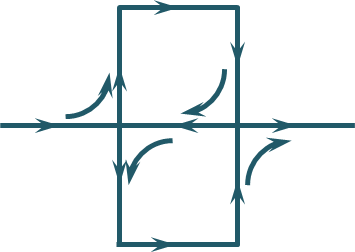
\includegraphics[width=.55\linewidth]{images/peano}
\end{center}

%\addcontentsline{toc}{subsection}{Exercice 10 -- Flocon de Koch}
\subsection*{Exercice 10 -- Flocon de Koch -- 4.6.32 p.123}
\begin{flushright}
\textit{D'après Frédéric Butin, l'informatique pas à pas en prépa, éditions ellipses.}
\end{flushright}
Le flocon de Koch est construit à partir d'un triangle équilatéral sur chacun des trois côtés duquel on applique les transformations suivantes : 
\begin{itemize}
\item on divise le côté en trois segments de même longueur;
\item on construit un triangle équilatéral ayant pour base le segment du milieu dont on supprime la base.
\end{itemize}
\begin{enumerate}
\item Si cela n'a pas été fait, s'approprier le module \texttt{turtle} en réalisant un cercle avec la tortue.
\item En utilisant la tortue de Python, écrire une procédure récursive qui reçoit un entier $n$ et trace le flocon de Koch en itérant $n$ fois le procédé décrit ci-dessus.
\end{enumerate}

\begin{center}
\begin{tabular}{ccc}
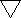
\includegraphics[width=.25\linewidth]{images/exo_FB_10_K1} &

\includegraphics[width=.25\linewidth]{images/exo_FB_10_K2} & 

\includegraphics[width=.25\linewidth]{images/exo_FB_10_K3} \\
\end{tabular}
\begin{tabular}{ccc}
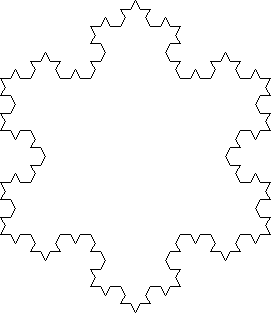
\includegraphics[width=.4\linewidth]{images/exo_FB_10_K4} & 
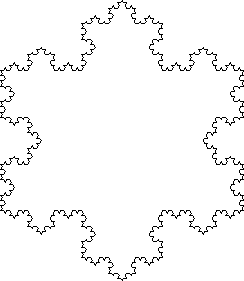
\includegraphics[width=.4\linewidth]{images/exo_FB_10_K5}
\end{tabular}
\end{center}

%\addcontentsline{toc}{subsection}{Exercice 11 -- Intégration numérique}
\subsection*{Exercice 11 -- Intégration numérique -- 4.6.33 p.124}
\begin{flushright}
\textit{D'après Frédéric Butin, l'informatique pas à pas en prépa, éditions ellipses.}
\end{flushright}

On considère la fonction $f:x \mapsto \ln x$.
\begin{enumerate}
\item Calculer $I=\int\limits_1^4 f(x) \text{d}x$.
\item Comparer l'erreur entre $I$ et la valeur approchée de $I$ obtenue par les méthodes des rectangles et des trapèzes en approchant un nombre de points $n$ où $n$ parcourt la suite $[10,20,40,100,200, 400, 500, 600, 700, 800, 900, 1000,$ $5000, 10000, 20000, 100000]$.
\item Représenter graphiquement cette erreur en prenant une échelle $\log$ -- $\log$. Expliquer les graphes obtenus.
\end{enumerate}

\begin{rem}
Tracé en diagramme log -- log :

\texttt{plt.loglog(x,y)}.
\end{rem}

%\addcontentsline{toc}{subsection}{Exercice 12 -- Équation différentielle}
\subsection*{Exercice 12 -- Équation différentielle -- 4.6.34 p.125}
\begin{flushright}
\textit{D'après Frédéric Butin, l'informatique pas à pas en prépa, éditions ellipses.}
\end{flushright}

Pour $n \in \mathbb{N}$, on considère l'équation différentielle : 
$$
x''(t) +10 x'(t) - x(t)=\sin \left( nt \right).
$$
\begin{enumerate}
\item Résoudre cette équation différentielle avec les conditions initiales $x(0)=0$ et $x'(0)=1$.
\item Représenter le graphe des solutions pour $n\in \llbracket 0,10 \rrbracket$ et $t \in[0,7]$.
\end{enumerate}

%\addcontentsline{toc}{subsection}{Exercice 13 -- Suite de Fibonacci}
\subsection*{Exercice 13 -- Suite de Fibonacci -- 4.6.41 p.135}
\begin{flushright}
\textit{D'après Frédéric Butin, l'informatique pas à pas en prépa, éditions ellipses.}
\end{flushright}

La suite de Fibonacci est la suite $\left( F_n \right)_{n \in \mathbb{N}}$ définie par $F_0=1$, $F_1=1$ et pour tout $n\in \mathbb{N}$, $F_{n+2}=F_{n+1}+F_{n}$.

\begin{enumerate}
\item Écrire une fonction qui calcule $F_n$ à l'aide de produits de matrice.
\item Déterminer la complexité de la procédure de la question précédente en nombre d'additions et en nombre de multiplications. On distinguera les cas où :
\begin{itemize}
\item la méthode d'exponentiation naïve est utilisée;
\item la méthode d'exponentiation rapide est utilisée.
\end{itemize}
\end{enumerate}


%\addcontentsline{toc}{subsection}{Exercice 14 -- Produits de matrices}
\subsection*{Exercice 14 -- Produits de matrices -- 4.6.42 p.136}
\begin{flushright}
\textit{D'après Frédéric Butin, l'informatique pas à pas en prépa, éditions ellipses.}
\end{flushright}
\begin{enumerate}
\item Calculer la complexité, en termes d'opérations sur les coefficients, de l'addition et de la multiplication de deux matrices de $M_n\mathbb{R}$ par la méthode naïve qui consiste à utiliser la définition du produit.

On suppose désormais que $n=2^k=2m$.
\item Une méthode de calcul de produit de deux matrices qui repose sur le principe << diviser pour régner >> est la suivante. On pose : 
$$
M=
\begin{bmatrix}
M_{11} & M_{12} \\
M_{21} & M_{22}
\end{bmatrix} 
\quad
\text{et}
\quad
N=
\begin{bmatrix}
N_{11} & N_{12} \\
N_{21} & N_{22}
\end{bmatrix} .
$$
On a donc :
$$
P=MN = 
\begin{bmatrix}
P_{11} & P_{12} \\
P_{21} & P_{22}
\end{bmatrix}
$$
avec :
$$
\begin{array}{ll}
P_{11} = M_{11}N_{11} + M_{12}N_{21} & 
P_{12} = M_{11}N_{12} + M_{12}N_{22} \\
P_{21} = M_{21}N_{11} + M_{22}N_{21} & 
P_{22} = M_{21}N_{12} + M_{12}N_{22}.
\end{array}
$$
Ainsi calculer le produit de deux matrices $M_n\mathbb{R}$ revient à calculer 8 produits de deux matrices de $M_{n/2}\mathbb{R}$.

Implémenter cet algorithme en une fonction \texttt{prod\_div}. Quelle est sa complexité ? Qu'en conclure ?
\item Une autre méthode de calcul consiste à poser 
$C_1 =M_{11}\left(N_{12} - N_{22} \right)$, 
$C_2 =N_{22}\left(M_{11} + M_{12} \right)$, 
$C_3 =N_{11}\left(M_{21} + M_{22}\right)$, 
$C_4 =M_{22}\left(N_{21} - N_{11} \right)$, 
$C_5 =\left(M_{11} + M_{22} \right) \left(N_{11} + N_{22} \right)$, 
$C_6 =\left(M_{12} - M_{22} \right)\left(N_{21} + N_{22} \right)$
et
$C_7 =\left(M_{11} - M_{21} \right)\left(N_{11} + N_{12} \right)$. Expliciter $P_{11}$, $P_{12}$, $P_{21}$ et $P_{22}$ en fonction des matrices $C_1$, ..., $C_7$. En déduire un algorithme (appelé algorithme de Strassen) permettant le calcul de $P=MN$ que l'on implémentera en une fonction \texttt{prod\_strassen}. Comparer la complexité de cet algorithme à celle des algorithmes des questions précédentes. 
\item Que faire quand $n$ n'est pas de la forme $2^k$ ?
\end{enumerate}


%\addcontentsline{toc}{subsection}{Exercice 15 -- Équations différentielles}
\subsection*{Exercice 15 -- Équations différentielles -- 4.6.46 p.144}
\begin{flushright}
\textit{D'après Frédéric Butin, l'informatique pas à pas en prépa, éditions ellipses.}
\end{flushright}
On souhaite résoudre par différences finies l'équation :
$$
u''(x)+2u(x) = 2 \cos x + \sin^2 x
$$
sur $[0,\pi]$ avec les conditions aux limites $u(0)=0$ et $u(\pi)=0$.

On considère la subdivision $0=x_0<x_1<...<x_n<x_{n+1} = \pi$ de l'intervalle $[0,\pi]$ où $x_i=ih$ et $h=\dfrac{\pi}{n+1}$. Pour tout $i$, on note $u_i$ la valeur approchée cherchée de $u(x_i)$ et on approche la dérivée seconde $u''(x)$ par :
$$
\dfrac{u_{i-1}-2u_i+u_{i+1}}{h^2}.
$$

\begin{enumerate}
\item Montrer que le système d'équation obtenu s'écrit matriciellement $AU=F$, où 
$$
A= 
\begin{bmatrix}
2h^2 - 2 & 1        & & & \\
1           & \ddots & \ddots & &  \\
& \ddots & \ddots &\ddots  & \\
& & \ddots & \ddots &1\\  
&& & 1 & 2h^2-2 \\
\end{bmatrix}
$$

$$
F=
\begin{bmatrix}
h^2 f(x_1) \\
\vdots \\
h^2 f(x_n)
\end{bmatrix}
\quad
U=
\begin{bmatrix}
u_1 \\
\vdots \\
u_n
\end{bmatrix}
$$
avec $f:x\mapsto 2 \cos x + \sin^2 x$.
\item Résoudre le système linéaire et représenter graphiquement la solution. 
\item La solution exacte de l'équation est :
$$
\begin{array}{lcl}
u(x)&=&\dfrac{\sin \left(\sqrt{2} x\right)  \left( 3+5 \cos \left(\sqrt 2 \pi \right)\right)}{2\sin \left(\sqrt{2} \pi\right)} \\
&&- \dfrac{5\cos \left(\sqrt{2} x\right)}{2}
+ \dfrac{\cos x}{2} \left( 4+\cos x\right)
\end{array}.
$$
Superposer le graphe de la solution exacte au graphe de la solution approchée.
\end{enumerate}


%\addcontentsline{toc}{subsection}{Exercice 16 -- Équations des ondes}
\subsection*{Exercice 16 -- Équations des ondes -- 4.6.47 p.146}
\begin{flushright}
\textit{D'après Frédéric Butin, l'informatique pas à pas en prépa, éditions ellipses.}
\end{flushright}
On souhaite résoudre par différences finies l'équation des ondes : 
$$
\partial_{tt} u(x,t) - c^2 \partial_{xx} u(x,t) = 0
$$

sur $[-5,5] \times [0,0.1]$ avec les conditions initiales $u(x,0)=\exp\left( {-10 x^2}\right)$ et 
$\partial_t u(x,0)=0$, et les conditions aux limites $u(-5,t)=u(5,t)=0$. 

On considère la subdivision $-5=x_0<x_1<\ldots <x_n <  x_{n+1} =5$ (resp. 
$0=t_0<t_i<\ldots<t_{m-1}<t_m=0,1$) de l'intervalle $[-5,5]$ (resp. $[0,0.1]$) où 
$x_i=-5+ih$ (resp. $t_k=kl$) et $h=\dfrac{10}{n+1}$ (resp. $l=\dfrac{0,1}{m}$).

Pour tout $(i,k) \in \llbracket 0,n+1 \rrbracket \times\llbracket 0,m \rrbracket $, on note $z_{i,k}$ la valeur approchée cherchée de $u\left(x_i,t_k\right)$ et l'on approche la dérivée première 
$\partial_{t} u(x_i,t_k)$ par $\dfrac{z_{i,k+1}-z_{i,k}}{l}$ et la dérivée seconde $\partial_{tt} u(x_i,t_k)$ par $\dfrac{z_{i,k+1}-2z_{i,k}+z_{i,k-1}}{l^2}$. On choisit $n=m=100$ et $c=31,6$.

\begin{enumerate}
\item Résoudre l'équation par différences finies en utilisant le schéma explicite, qui consiste à approcher la dérivée seconde $\partial_{xx} u(x_i,t_k)$ par l'expression $\dfrac{z_{i-1,k}-2z_{i,k}+z_{i+1,k}}{h^2}$.
\item Créer une animation permettant de visualiser la solution obtenue quand $t$ varie. 
\item Résoudre l'équation par différences finies en utilisant le schéma implicite, qui consiste à approcher la dérivée seconde $\partial_{xx} u(x_i,t_k)$ par l'expression :
$\dfrac{z_{i-1,k+1}-2z_{i,k+1}+z_{i+1,k+1}}{h^2}$.
\item Créer une animation permettant de visualiser la solution obtenue quand $t$ varie. 
\end{enumerate}

%\addcontentsline{toc}{subsection}{Exercice 17 -- Position d'une membrane}
\subsection*{Exercice 17 -- Position d'une membrane -- 4.6.49 p.153}
\begin{flushright}
\textit{D'après Frédéric Butin, l'informatique pas à pas en prépa, éditions ellipses.}
\end{flushright}

On considère une membrane élastique dont le bord est fixé à un cadre carré horizontal. La membrane est soumise à une force verticale $f$. On peut montrer que l'altitude$z(x,y)$ de la membrane en un point du carré de coordonnées $(x,y)$ vérifie l'équation de Laplace :
$$
\Delta z\left( x,y\right) = f(x,y)
$$
 avec les conditions aux limites $z(x,y)=0$ sur le bord du carré. 
 
 On se place dans le cas où le cadre est le carré $[0,1]^2$ et où$f$ est constante, par exemple $f(x,y)=-4$ pour tout $(x,y)\in[0,1]^2$. 
 
 Pour résoudre cette équation par la discrétisation, on pose $h=\dfrac{1}{n+1}$ et pour tout $(i,j)\in \llbracket 0,n+4 \rrbracket^2$, $x_i=ih$ et $y_j=jh$: on obtient ainsi un quadrillage du carré $[0,1]^2$. On a déjà $z\left(x_i,y_j\right)=0$  si $i\in \{0,n+1\}$ ou $j \in \{0,n+1\}$ par hypothèse. On note $z_{i,j}$ l'approximation cherchée de $z\left(x_i,y_j\right)$ par $z_{i,j}$ et le laplacien $\Delta z\left(x_i,y_j\right)$ par son approximation à 5 points : 
 
 $$
 \dfrac{1}{h^2}\left( z_{i-1,j}+z_{i+1,j}+z_{i,j-1}+z_{i,j+1}-4z_{i,j}\right).
 $$
 
 On résout alors le système formé par les équations obtenues, qui est un système linéaire dont les inconnues sont les $z_{i,j}$ pour $(i,j)\in 
  \llbracket 0,1 \rrbracket^2$.
\begin{enumerate}
\item Étant donné $A=\left(a_{i,j}\right)_{(i,j)\in\llbracket 1,n \rrbracket^2 }$ et $B=\left(b_{i,j}\right)_{(i,j)\in\llbracket 1,n \rrbracket^2 }$ deux matrices de $M_n\mathbb{R}$, le produit de Kronecker $de$ A par $B$ est la matrice de $M_{n^2}\mathbb{R}$ définie par :
$$
A\otimes B = 
\begin{bmatrix}
a_{1,1}B & a_{1,2}B & \ldots & a_{1,n}B \\
a_{2,1}B & a_{2,2}B & \ldots & a_{2,n}B \\
\vdots  & & & \vdots  \\
a_{n,1}B & a_{n,2}B & \ldots & a_{n,n}B \\
\end{bmatrix} .
$$
La commande \texttt{kron} de numpy permet de calculer le produit de Kronecker. Observer que le système linéaire peut se mettre sous la forme $\left(A_n\otimes I_n+ I_n\otimes A_n\right)Z=F$ où $A_n$ est la matrice du laplacien de taille $n$, c'est à dire : 
$$
A_n = 
\begin{bmatrix}
2  & -1 & & \\
-1 & \ddots & \ddots & \\
   & \ddots &\ddots & -1\\
   &  & -1& 2\\
\end{bmatrix} .
$$
\item Résoudre l'équation par discrétisation, comme expliqué ci-dessus.
\item Représenter la membrane en 3d.
\end{enumerate}  


%\addcontentsline{toc}{subsection}{Exercice 18 -- Polygones orthogonaux}
\subsection*{Exercice 18 -- Polygones orthogonaux -- 4.6.50 p.155}
\begin{flushright}
\textit{D'après Frédéric Butin, l'informatique pas à pas en prépa, éditions ellipses.}
\end{flushright}
\begin{enumerate}
\item Pour $n=16$, créer en Python la base canonique de $\mathbb{R}_n[X]$. 
\item Définir le produit scalaire $\varphi : \left( P,Q\right) \mapsto \int\limits_{-1}^{1} P(t) Q(t) \text{d}t$ et la norme euclidienne associée sur $\mathbb{R}_n[X]$. 
\item En utilisant le procédé de Gram-Schmidt, orthonormaliser la  base canonique pour le produit scalaire $\varphi$.
\item Calculer la projection orthogonale de $h:x\mapsto \cos \left( 4\pi x\right)$ sur $\mathbb{R}_n[X]$ (approximation de $h$ au sens des moindres carrés).
\end{enumerate}


%\addcontentsline{toc}{subsection}{Exercice 19 -- Système proies -- prédateurs}
\subsection*{Exercice 19 -- Système proies -- prédateurs -- 4.6.37 p.129}
\begin{flushright}
\textit{D'après Frédéric Butin, l'informatique pas à pas en prépa, éditions ellipses.}
\end{flushright}
Le système proies-prédateurs est régit par les équations de Volterra qui forment le système non linéaire :
$$
\left\{
\begin{array}{l}
x'(t)=ax(t)-bx(t)y(t) \\
y'(t)=-cy(t)+dx(t)y(t) \\
\end{array}
\right. ,
$$
où $a$, $b$, $c$ et $d$ sont des réels strictement positifs. 
\begin{enumerate}
\item On pose $X=(x,y)^t$. Créer une fonction $f$ qui à $(X,t,a,b,c,d)$ fait correspondre $(ax-bxy,-cy+dxy)$.
\item Résoudre le système dans les conditions suivantes : $X=(1,2)$ et $a,b,c,d=1,1,1,1$. 
\item Représenter $x$ et $y$ sur un même graphique. 
\item Représenter les courbes paramétrées par $x$ et $y$, qui donne l'évolution des deux populations.
\end{enumerate}

%\addcontentsline{toc}{subsection}{Exercice 20 -- Transformée de Fourier}
\subsection*{Exercice 20 -- Transformée de Fourier -- 4.6.65 p.241.}
\begin{flushright}
\textit{D'après Frédéric Butin, l'informatique pas à pas en prépa, éditions ellipses.}
\end{flushright}
Implémenter en Python l'algorithme naïf de calcul de la transformée de Fourier d'un vecteur de $\mathbb{C}^N$.

%\addcontentsline{toc}{subsection}{Exercice 21}
\subsection*{Exercice 21 -- 6.5.66 p.242.}
\begin{flushright}
\textit{D'après Frédéric Butin, l'informatique pas à pas en prépa, éditions ellipses.}
\end{flushright}
Soit $f:\mathbb{R} \to \mathbb{R}$ l'application $2\pi$-périodique définie par :
$$
f(x)=\left\{
\begin{array}{l}
1  \quad \text{si} \quad x\in[0,\pi[ \\
10  \quad \text{si} \quad x\in[\pi,2\pi[
\end{array}
\right. .
$$
\begin{enumerate}
\item En utilisant la FFT, calculer des valeurs approchées des coefficients de Fourier de $f$. 
\item Représenter sur un même graphique $f$ et la somme approchée de sa série de Fourier.
\end{enumerate}

%\addcontentsline{toc}{subsection}{Exercice 22 -- Débruitage d'un signal}
\subsection*{Exercice 22 -- Débruitage d'un signal -- 6.5.65 p.243.}
\begin{flushright}
\textit{D'après Frédéric Butin, l'informatique pas à pas en prépa, éditions ellipses.}
\end{flushright}
On considère un signal donné par l'application :
$$
f:t \mapsto 3 \cos \left( 3t\right)+2\sin \left( 2t\right)-\dfrac{1}{2}\cos t
$$
échantillonné sur $n=100$  points équidistants $(t_k)_{k\in \llbracket 1,n\rrbracket}$ du segment $[0,2\pi]$. On introduit sur ce signal un bruit donné par une loi uniforme sur $[-1,1]$ : ainsi pour tout point $t_k$ d'échantillonnage, la valeur du signal n'est pas $f(t_k)$, mais $g(t_k) = f(t_k) + b_k$, où $b_k$ est une réalisation d'une loi uniforme sur $[-1,1]$.

\begin{enumerate}
\item Représenter sur un même graphique le signal $f$ et le signal bruité $g$.
\item Appliquer la FFT au signal bruité. Construire alors un nouveau signal débruité $h$ en supprimant les fréquences d'indices trop grands (on peut par exemple ne garder qu'un quart des fréquences).
\item Représenter $h$ sur le même graphique que $f$ et $g$.
\end{enumerate}

%\addcontentsline{toc}{subsection}{Exercice 23 -- Taches solaires}
\subsection*{Exercice 23 -- Taches solaires -- 4.6.65 p.244.}
\begin{flushright}
\textit{D'après Frédéric Butin, l'informatique pas à pas en prépa, éditions ellipses.}
\end{flushright}
Nous nous intéressons ici aux mesures de l'activité des taches solaires de l'année 1700 à l'année 2004. On appelle nombre de Wolf le nombre de taches solaires observées en une année. %Les données, écrites sous la forme [année, nombre Wolf], sont regrou

La transformée de Fourier, qui permet de passer du domaine temporel au domaine fréquentiel, donne la possibilité de savoir s'il existe une fréquence prédominante, c'est-à-dire si les données sont périodiques.

\begin{enumerate}
\item Représenter graphiquement le nombre Wolf en fonction de l'année. 
\item Effectuer la FFT de la liste des nombres de Wolf. On la note $Y$.Représenter alors $\mathfrak{I}\left(Y\right)$ en fonction de $\mathfrak{R}\left(Y\right)$.
\item On souhaite construire un chronogramme, c'est-à-dire une graphe de la puissance du signal en fonction de la fréquence (la puissance de la FFT étant égale au carré du signal de la FFT). 

Tracer ce chronogramme en utilisant uniquement les coefficients de $Y$ compris entre 1 et $E\left(\dfrac{n}{2}\right)$, où $n$ est le nombre de relevés (les coefficients situés au-delà de $E\left(\dfrac{n}{2}\right)$ correspondant à des coefficients de Fourier d'indices négatifs) : la plage de fréquences est donc :

$$
\left( \dfrac{k}{n} \right)_{k\in \llbracket 1, E\left(\dfrac{n}{2}\right) \rrbracket} = \left[ \dfrac{1}{n},\dfrac{2}{n},\ldots E\left(\dfrac{n}{2}\right) \dfrac{1}{n}\right].
$$

Tracer le graphe de la puissance du signal en fonction de la période. Que constate-t-on ?
\end{enumerate}

%\addcontentsline{toc}{subsection}{Exercice 24 -- Traitement d'image -- Filtre}
\subsection*{Exercice 24 -- Traitement d'image -- Filtre -- 6.5.69 p.247.}
\begin{flushright}
\textit{D'après Frédéric Butin, l'informatique pas à pas en prépa, éditions ellipses.}
\end{flushright}

\begin{enumerate}
\item Créer une fonction qui permet d'afficher la composante rouge d'une image. 
\item Créer une fonction qui permet d'afficher la composante cyan.
\end{enumerate}

\end{multicols}



\newpage 
%\begin{multicols}{2}

\section{Corrigés -- Banque PT}
%\addcontentsline{toc}{subsection}{Exercice 1 -- Arithmétique -- Corrigé}
\subsection*{Exercice 1 -- Arithmétique -- Corrigé}

\begin{corrige}
$\quad$
\begin{python}
# Question 1
n = 1234
q = n//10
r =  n%q

# r contient le nombre d'unités de n
\end{python}
\end{corrige}

\begin{corrige}
$\quad$
\begin{python}
# Question 2
s=0
while n!=0:
    q=n//10
    r = n%10
    #print(r)
    s=s+r**3
    n=q
\end{python}
\end{corrige}

\begin{corrige}
$\quad$
\begin{python}
# Question 3
def somcube(n):
    """
    Entrées :
     * n, int : nombre
    Sortie : 
     * s, int : somme des cubes du chiffre n
    """
    s=0
    while n!=0:
        q=n//10
        r = n%10
        s=s+r**3
        n=q
    return s
\end{python}
\end{corrige}

\begin{corrige}
$\quad$
\begin{python}
# Question 4
res = []
for i in range (10001):
    if i == somcube(i):
        res.append(i)
\end{python}
\end{corrige}

\begin{corrige}
$\quad$
\begin{python}
# Question 5
def somcube2(n):
    """
    Entrées :
     * n, int : nombre
    Sortie : 
     * s, int : somme des cubes du chiffre n
    """
    nombre=str(n)
    s=0
    for chiffre in nombre :
        s = s+int(chiffre)**3
    return s
    
print(somcube2(1234))
\end{python}
\end{corrige}

%\vfill

%%\columnbreak

%\addcontentsline{toc}{subsection}{Exercice 2 -- Intégration -- Corrigé}
\subsection*{Exercice 2 -- Intégration -- Corrigé}

\begin{corrige}
$\quad$
\begin{python}
# Question 1
# ==========
# Le répertoire courant est Exercice_02.
# Le sous-répertoire data contient le
# fichier ex_02.txt.

# On ouvre le fichier en lecture)
fid = open("data\ex_02.txt")

# On charge le fichier dans une liste.
# Chaque élément de la liste correspond à 
# chaque ligne sous forme de chaîne de caractère.
file = fid.readlines()
# On ferme le fichier
fid.close()

LX=[]
LY=[]
for ligne in file :
    ligne = ligne.split(';')
    LX.append(float(ligne[0]))
    LY.append(float(ligne[1]))
\end{python}
\end{corrige}

\begin{corrige}
$\quad$
\begin{python}
# Question 2
# ==========
# Ne pas oublier de charger préalablement 
# import matplotlib.pyplot as plt

plt.plot(LX,LY)
plt.show()
\end{python}
\end{corrige}
\begin{center}
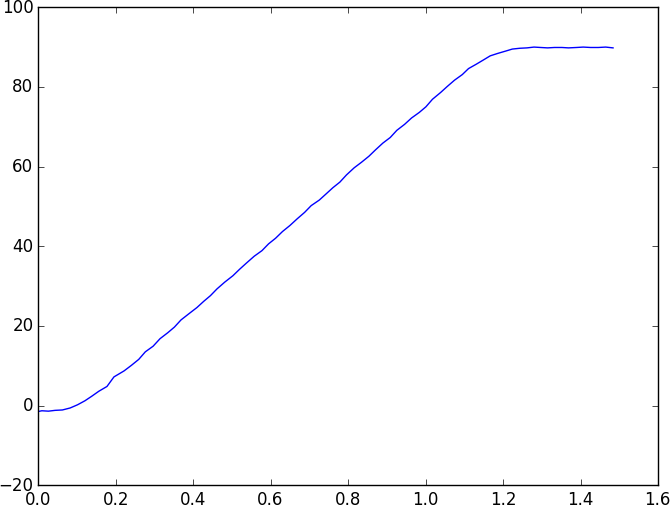
\includegraphics[width=6cm] {images/exo_02}
\end{center}


\begin{corrige}
$\quad$
\begin{python}
# Question 3
# ==========
def trapeze(x,y):
    res = 0 
    for i in range(1,len(LX)):
        res = res+(LX[i]-LX[i-1])*0.5*(LY[i]+LY[i-1])
    return res
print(trapeze(LX,LY))

>>> 75.13635
\end{python}
\end{corrige}

\begin{corrige}
$\quad$
\begin{python}
# Question 4
# ==========
from scipy.integrate import trapz
# Attention à l'ordre des arguments dans 
# la fonction trapz : les_y puis les_x
# Après l'import, help(trapz) permet d'avoir 
# de l'aide sur la fonction.
print(trapz(LY,LX))

>>> 75.13635
\end{python}
\end{corrige}

%\addcontentsline{toc}{subsection}{Exercice 3 -- Graphe -- Corrigé}
\subsection*{Exercice 3 -- Graphe -- Corrigé}

\begin{corrige}
$\quad$
\begin{python}
# Question 1
# ==========
# Matrices avec des listes
M=[[0,9,3,-1,7],
      [9,0,1,8,-1],
      [3,1,0,4,2],
      [-1,8,4,0,-1],
      [7,-1,2,-1,0]]
\end{python}
\end{corrige}
%\newpage

\begin{corrige}
$\quad$
\begin{python}
# Question 2 & 3
# ==============
def voisins(M,i):
    """
    Entrées : 
      * M(lst) : graphe
      * i : noeud considéré
    Sortie :
      * v(lst) : liste des voisins
    """
    v = []
    # On cherche les voisins sur une ligne 
    # (on pourrait le faire sur une colonne)
    for j in range(len(M[i])):
        if M[i][j]>0:
            v.append(j)
    return v
    
# print(voisins(M,0))
\end{python}
\end{corrige}


\begin{corrige}
$\quad$
\begin{python}
# Question 4
# ==========
def degre(M,i):
    """
    Entrées : 
      * M(lst) : graphe
      * i : noeud considéré
    Sortie :
      * (int) : nomnbre de voisins
    """
    return len(voisins(M,i))
\end{python}
\end{corrige}

\begin{corrige}
$\quad$
\begin{python}
# Question 5
# ==========
def longueur(M,chemin):
    l = 0
    for i in range(len(chemin)-1):
        if M[chemin[i]][chemin[i+1]]<0:
            return -1
        else :
            l=l+M[chemin[i]][chemin[i+1]]
    return l
    
chemin = [1,2,3,1,4]
print(longueur(M,chemin))        
chemin = [0,4,2,1,0]
print(longueur(M,chemin))
\end{python}
\end{corrige}

\vfill

%\columnbreak
%\addcontentsline{toc}{subsection}{Exercice 4 -- Corrigé}
\subsection*{Exercice 4 -- Corrigé}
\begin{corrige}
$\quad$
\begin{python}
# Question 1 
# ==========
def nombreZeros(t,i):
    if t[i]==1:
        return 0
    else : 
        res = 1
        j=i+1
        while j<len(t) and t[j]==0:
            res = res+1
            j=j+1
    return res
# t1=[0,1,1,1,0,0,0,1,0,1,1,0,0,0,0]
# print(nombreZeros(t1,4))
# print(nombreZeros(t1,1))
# print(nombreZeros(t1,8))
\end{python}
\end{corrige}

\begin{corrige}
$\quad$
\begin{python}
# Question 2
# ==========
def nombreZerosMax(t):
    max=nombreZeros(t,0)
    for i in range(1,len(t)):
        tmp = nombreZeros(t,i)
        if tmp>max:
            max = tmp
    return max
print(nombreZerosMax(t1))
\end{python}
\end{corrige}

\begin{corrige}
La complexité est quadratique ($\mathcal{O}^2$)  du fait de la boucle \texttt{for} et de la boucle \texttt{while} imbriquée.

Pour diminuer la complexité, il est possible de parcourir une seule fois la liste. On lit alors les termes un à un. Quand on détecte un zéro, on compte alors le nombre de zéros consécutifs et on poursuit jusqu'à la fin...

\end{corrige}

%\addcontentsline{toc}{subsection}{Exercice 5 -- Corrigé}
\subsection*{Exercice 5 -- Corrigé}
D'après Mme Barré \url{http://www.lycee-lesage.net/}.


\begin{corrige}
$\quad$
\begin{python}
import math
import scipy.misc as scim
# Question 1 
# ==========
def Px_poisson(k, n, p):
    """
    Entrée : 
     * k(int)
     * n(int) : strictement positif
     * p(flt) : réel compris entre ]0, 1[
    X suit une loi de Poisson P(n*p)
    Sortie : 
     * flt : (np)^k exp(-np)/k!
    """
    np = n * p
    return (np)**k * math.exp(- np) / math.factorial(k)

n, p = 30, 0.1
lst_px = [Px_poisson(k, n, p) for k in range(n + 1)]
\end{python}
\end{corrige}

\begin{corrige}
$\quad$
\begin{python}
# Question 2
# ==========
def Py_binomiale(k, n, p):
    """
    Entrée : 
     * k(int)
     * n(int) : strictement positif
     * p(flt) : réel compris entre ]0, 1[
    Y suit une loi binomiale B(n,k)
    Sortie : 
     * int : B(n,k)*p^k *(1-p)^(n-k)
    """
    return scim.comb(n,k)*p**k*(1-p)**(n-k)

n, p = 30, 0.1
lst_py = [Py_binomiale(k, n, p) for k in range(n + 1)]
\end{python}
\end{corrige}

\begin{corrige}
$\quad$
\begin{python}
# Question 3
# ==========
def ecarts(n,p):
	"""
	Entrée :
     * n(int) : strictement positif
     * p(flt) : réel compris entre ]0, 1[
    Sortie : 
     * maxi(flt) écart maxi entre P(Y=k) et P(X=k)
    """
     
	lst_px = [Px_poisson(k, n, p) for k in range(n + 1)]
    lst_py = [Py_binomiale(k, n, p) for k in range(n + 1)]
    maxi = max([abs(lst_py[i]-lst_px[i]) for i in range(len(lst_px))])
    return maxi
    
#print(ecarts(n,p))
\end{python}
\end{corrige}

\begin{corrige}
$\quad$
\begin{python}
# Question 4
# ==========
def E(e,p):
	"""
	Retourne le plus petit entier naturel n tq ecart(n,p)<=e
	Entrée : 
	 * e(flt) : >0
	 * p(flt) : réel compris entre ]0, 1[
    Sortie :
     n(int)
	"""
	n=1
	while (ecarts(n,p))>e :
		n=n+1
	return n
\end{python}
\end{corrige}

\begin{corrige}
$\quad$
\begin{python}
# Question 5
# ==========
print(E(0.008,0.075))
print(E(0.005,0.075))
print(E(0.008,0.1))
#print(E(0.005,0.1))
\end{python}
\end{corrige}



%\columnbreak 

%\addcontentsline{toc}{subsection}{Exercice 6 -- Corrigé}
\subsection*{Exercice 6 -- Corrigé}
\begin{corrige}
$\quad$
\begin{python}
# Import de fonctions
import matplotlib.pyplot as plt
from math import sqrt
# Question 1 
# ==========
def g(x):
    if x>= 0 and x<1 :
        return x
    elif x>1 and x<2 :
        return 1
xx = [0]
t=0
while t<=1.99:
    t=t+0.01
    xx.append(t)
yy = [g(x) for x in xx]
plt.plot(xx,yy)
plt.show()
\end{python}
\end{corrige}

\begin{corrige}
$\quad$
\begin{python}
# Question 2
# ==========
def f(x):
    if x>=0 and x<2 :
        return g(x)
    else : # x>=2
        return sqrt(x)*f(x-2)
\end{python}
\end{corrige}

\begin{corrige}
$\quad$
\begin{python}
# Question 3
# ==========
xxx = [0]
t=0
while t<=6:
    t=t+0.01
    xxx.append(t)
yyy = [f(x) for x in xxx]
plt.plot(xxx,yyy)
plt.show()
\end{python}
\end{corrige}

%\columnbreak 

\begin{corrige}
$\quad$
\begin{python}
# Question 4
# ==========
# On cherche à résoudre f(x)-4 = 0 sur
# l'intervalle [5,6]
def h(x):
    res = f(x)-4
    return res

a = 5.
b = 6.
while (b-a)>0.01:
    m=(a+b)/2
    if h(m)>0:
        b=m
    else :
        a=m
m=(a+b)/2

if h(m)<0:
    m= m+ abs(b-a)
print(m,h(m))
\end{python}
\end{corrige}
 

%\addcontentsline{toc}{subsection}{Exercice 7 -- Corrigé}
\subsection*{Exercice 7 -- Corrigé}

\begin{corrige}
$\quad$
\begin{python}
# Question 1 
# ==========
def d(n):
    """
    Retourne la liste de tous les diviseurs de n.
    Entrée : 
     * n(int) : entier.
    Sortie : 
     * L(lst) : liste des diviseurs de n.
    """
    L =[1]
    for nombre in range(2,n+1):
        if n%nombre == 0:
            L.append(nombre)
    return L
print(d(4),d(10))
\end{python}
\end{corrige}

\begin{corrige}
$\quad$
\begin{python}
# Question 2 
# ==========
def DNT_01(n):
    return d(n)[1:-1]
def DNT_02(n):
    L =[]
    for nombre in range(2,n):
        if n%nombre == 0:
            L.append(nombre)
    return L
print(DNT_01(4),DNT_02(4))
print(DNT_01(10),DNT_02(10))
\end{python}
\end{corrige}


\begin{corrige}
$\quad$
\begin{python}
# Question 3
# ==========
def sommeCarresDNT_01(n):
    L = DNT_01(n)
    res = [x**2 for x in L]
    return sum(res)
def sommeCarresDNT_02(n):
    L = DNT_01(n)
    res = 0
    for x in L:
        res = res + x*x
    return res
def sommeCarresDNT_03(n):
    L = DNT_01(n)
    res = 0
    for i in range(len(L)):
        res = res + L[i]**2
    return res
print(sommeCarresDNT_01(15),sommeCarresDNT_02(15),
    sommeCarresDNT_03(15))
\end{python}
\end{corrige}


\begin{corrige}
$\quad$
\begin{python}
# Question 4
# ==========
from math import sqrt
for i in range(1001):
    if i == sommeCarresDNT_01(i) :
        print(str(i)+"\t"+str(sqrt(i)))
# Conjecture les nombres recherchés sont 
# les carrés des nombres premiers. 
\end{python}
\end{corrige}


%\addcontentsline{toc}{subsection}{Exercice 8 -- Corrigé}
\subsection*{Exercice 8 -- Corrigé}
\begin{corrige}
$\quad$
\begin{python}
# Question 1 
# ==========
chaine = "abcdefghijklmnopqrstuvwxyz"
\end{python}
\end{corrige}

\begin{corrige}
$\quad$
\begin{python}
# Question 2
# ==========
def decalage(chaine,n):
    chaine = chaine[n:-1]+chaine[0:n]
    return chaine
print(chaine,decalage(chaine,3))
\end{python}
\end{corrige}

\begin{corrige}
$\quad$
\begin{python}
# Question 3
# ==========
def indices(x,phrase):
    """
    Recherche des indices de x dans phrase
    Entrée : 
     * x(str) : un caractère
     * phrase(str)
    Sortie : 
     * res(lst) : liste des indices de x
    """
    res = []
    for i in range(len(phrase)):
        if phrase[i] == x:
            res.append(i)
    return res

print(indices("a","akjlkjalkjlkjalkjlkja"))
\end{python}
\end{corrige}

\begin{corrige}
$\quad$
\begin{python}
# Question 4
# ==========
def codage(n,phrase):
    ch = "abcdefghijklmnopqrstuvwxyz"
    ch_c = decalage(ch,n)
    print(ch_c)
    phrase_c=""
    for c in phrase :
        i = indices(c,ch)
        i = i[0]
        phrase_c = phrase_c+ch_c[i]
    return phrase_c
print(codage(3,"oralensam"))
\end{python}
\end{corrige}

\begin{corrige}
$\quad$
\begin{python}
# Question 5
# ==========
# Solution 1 : essayer les 26 permutations, 
# jusqu'à trouver une phrase qui est du sens.
# Solution 2 : statistiquement le e est la lettre
# la plus présente dans la langue française. On
# peut donc déterminer la fréquence d'apparition 
# des lettres. # La lettre la plus fréquente 
# peut être assimilée au "e".
# On calcule ainsi le décalage...
\end{python}
\end{corrige}

%\addcontentsline{toc}{subsection}{Exercice 9 -- Fractale de Mandelbrot -- Corrigé}
\subsection*{Exercice 9 -- Fractale de Mandelbrot -- Corrigé}
\begin{corrige}
$\quad$
\begin{python}
# Question 1 
# ==========
def suite_u(c,n):
    """
    Calcul de la suite u au rang n.
    Entrées : 
     * c(flt) : nombre quelconque
     * n(int)
    Sortie : 
     * res(flt) : valeur de u(n)
    """
    res = 0
    i=0
    while i!=n:
        res = res*res+c
        i=i+1
    return res
\end{python}
\end{corrige}

\begin{corrige}
$\quad$
\begin{python}
def recherche_k(m,M,c):
    """ Recherche de k """
    k=0
    while k<=m:
        if abs(suite_u(c,k))>M:
            return k
        k=k+1
    return -1
\end{python}
\end{corrige}

\begin{corrige}
$\quad$
\begin{python}
def fonction_f(m,M,c):
    """ Fonction """
    k = recherche_k(m,M,c)
    if k>=0:
        return k
    else :
        return m+1
\end{python}
\end{corrige}

\begin{corrige}
$\quad$
\begin{python}
# Question 2
#===========
import matplotlib.pyplot as plt
m,M=10,20
LX = [-2+4*x/400 for x in range(401)]
LF = [fonction_f(m,M,x) for x in LX]
plt.plot(LX,LF,"*")
plt.show()
\end{python}
\end{corrige}
\begin{center}
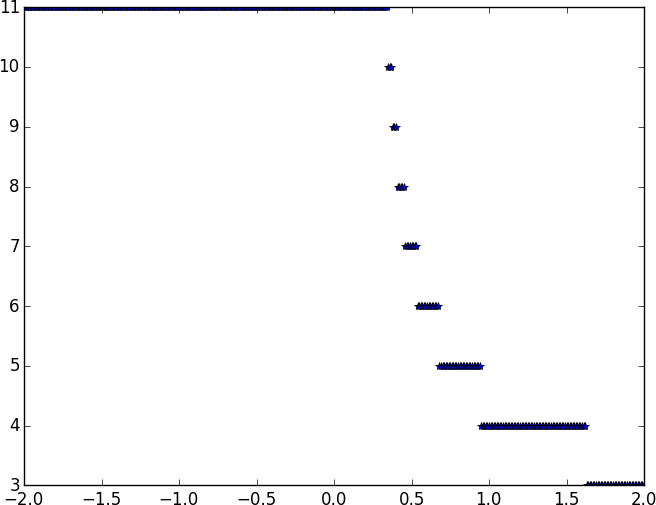
\includegraphics[width=.4\linewidth]{programmes/Exercice_09/figure_1}
\end{center}
\begin{corrige}
$\quad$
\begin{python}
# Question 3
#===========
LX = [-2+2.5*x/100 for x in range(101)]
LY = [-1.1+2.2*x/100 for x in range(101)]
XY = [[[x,y] for x in LX] for y in LY]

for i in range(len(LX)):
    for j in range(len(LY)):
        XY[i][j]=fonction_f(
            m,M,complex(XY[i][j][0],XY[i][j][1]))
\end{python}
\end{corrige}

\begin{corrige}
$\quad$
\begin{python}

# Question 4
#===========
res = 100
LX = [-2+2.5*x/res for x in range(res+1)]
LY = [-1.1+2.2*x/res for x in range(res+1)]
XY = [[[x,y] for x in LX] for y in LY]

for i in range(len(LX)):
    for j in range(len(LY)):
        XY[i][j]=fonction_f(
        m,M,complex(XY[i][j][0],XY[i][j][1]))

# plt.imshow(XY)
# plt.show()
\end{python}
\end{corrige}

\begin{corrige}
$\quad$
\begin{python}

# Bilan 
#=======
def affichage(m,M,res):
    m = m
    M = M
    LX = [-2+2.5*x/res for x in range(res+1)]
    LY = [-1.1+2.2*x/res for x in range(res+1)]
    XY = [[[x,y] for x in LX] for y in LY]
    for i in range(len(LX)):
        for j in range(len(LY)):
            XY[i][j]=fonction_f(
                m,M,complex(XY[i][j][0],XY[i][j][1]))
    plt.imshow(XY)
    plt.show()
\end{python}
\end{corrige}

\begin{center}
\begin{tabular}{ccc}
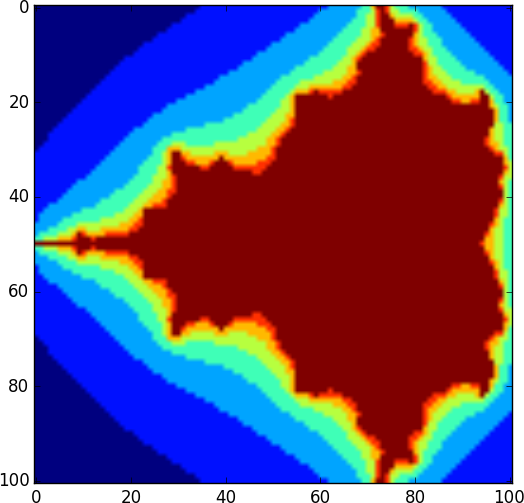
\includegraphics[width=.3\linewidth]{programmes/Exercice_09/10_20_100} &
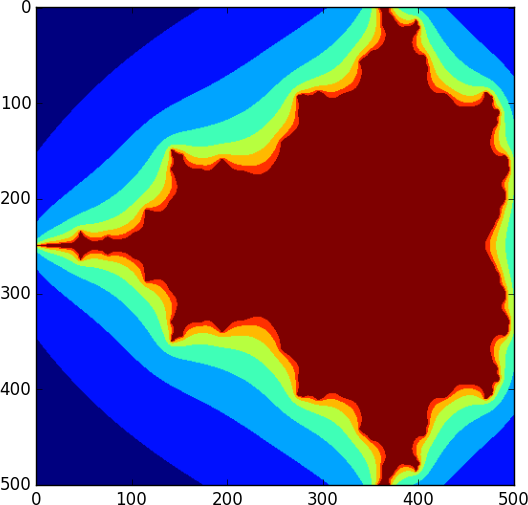
\includegraphics[width=.3\linewidth]{programmes/Exercice_09/10_20_500} & 
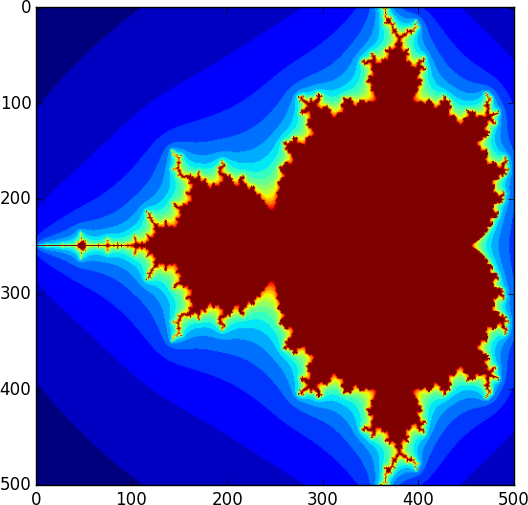
\includegraphics[width=.3\linewidth]{programmes/Exercice_09/20_40_500} \\
\textit{$m=10$, $M=20$} &
\textit{$m=10$, $M=20$} &
\textit{$m=20$, $M=40$} \\
\textit{100 points par 100 points} & 
\textit{500 points par 500 points} & 
\textit{500 points par 500 points} \\
\end{tabular}
\end{center}


%\columnbreak 

%\addcontentsline{toc}{subsection}{Exercice 10 -- Corrigé}
\subsection*{Exercice 10 -- Corrigé}
\begin{corrige}
$\quad$
\begin{python}
import numpy as np
# Question 1
R = np.array([[1,2,3],[4,5,6]])
S = np.array([[1,2,3],[4,5,6],[7,8,9]])
\end{python}
\end{corrige}

\begin{corrige}
$\quad$
\begin{python}
# Question 2
def test(M):
    """
    Fonction permettant de tester si la
    matrice est carrée et retournant sa taille.
    Entrée : 
     * M(numpy.ndarray) : matrice
    Sortie :
     * 0 si taille non carrée
     * n(int) : taille de M si elle est carrée
    """
    l = M.shape[0]
    c = M.shape[1]
    if l==c :
        return l
    else : 
        return 0
print(test(R),test(S))
\end{python}
\end{corrige}

\begin{corrige}
$\quad$
\begin{python}
# Question 3
fid = open("data/ex_006.txt",'r')
M1 = []
for ligne in fid :
    l = ligne.rstrip().split(" ")
    Ligne = [float(x) for x in l]
    M1.append(Ligne)
fid.close()
M1 = np.array(M1)
\end{python}
\end{corrige}

\begin{corrige}
$\quad$
\begin{python}
# Question 4
if test(M1)>0:
    valeurs_propres = np.linalg.eig(M1)[0]
    print(valeurs_propres)
\end{python}
\end{corrige}

\begin{corrige}
$\quad$
\begin{python}
# Question 5
def dansIntervalle(L,a,b):
    """
    Vérifier que chaque élément de L est dans 
    l'intervalle [a,b]
    Entrées : 
     * L(lst) : liste de nombres
     * a,b(flt) : nombres
    Sortie : 
     * True si chaque élément est dans [a,b]
     * False sinon. 
    """   
    for e in L :
        if e<a or e> b:
            return False
    return True
print(dansIntervalle(valeurs_propres,0,1))
\end{python}
\end{corrige}

%\addcontentsline{toc}{subsection}{Exercice 11 -- Tri de liste -- Corrigé}
\subsection*{Exercice 11 -- Tri de liste -- Corrigé}

\begin{corrige}
$\quad$
\begin{python}
# Question 1 
# ==========
def comptage(L,n):
    """
    Comptage des éléments de L.
    Entrées :
     * n(int) : entier
     * L(lst) : liste d'éléments inférieurs à n
    """
    P = [0 for i in range(n+1)]
    # P = [0]*(n+1)
    for e in L:
        P[e]=P[e]+1
    return P
from random import randint
maxi = 5
LL = [randint(0,maxi) for x in range(20)]
P = comptage(LL,maxi)
# print(LL)
# print(P)
\end{python}

\end{corrige}

\begin{corrige}
$\quad$
\begin{python}
# Question 2
# ==========
def tri(L,n):
    """
    Tri une liste.
    Entrées :
     * n(int) : entier
     * L(lst) : liste d'éléments inférieurs à n
    Sortie : 
     * T(lst) : liste triée.
    """
    P = comptage(L,n)
    T = []
    for i in range(len(P)):
        for j in range(P[i]):
            T.append(i)
    return T
\end{python}
\end{corrige}

\begin{corrige}
$\quad$
\begin{python}
# Question 3
# ==========
from random import randint
maxi = 5
LL = [randint(0,maxi) for x in range(20)]
T = tri(LL,maxi)
print(LL)
print(T)
\end{python}
\end{corrige}

\begin{corrige}
$\quad$
\begin{python}
# Question 4
# ==========
# Complexité quadratique : C(n)=O(n+n^2)=O(n^2)
# n : complexité de comptage
# n^2 : complexité des deux boucles imbriquées du 
# tri
# Ce tri s'exécutera toujours dans le pire des cas.
# Dans le cas moyen : tri fusion O(nlogn)
# Dans le cas moyen : tri insertion O(n^2)
\end{python}
\end{corrige}
 
%\columnbreak

%\addcontentsline{toc}{subsection}{Exercice 12 -- Corrigé}
\subsection*{Exercice 12 -- Corrigé}

\begin{corrige}
$\quad$
\begin{python}
b,w = 0.5,6
# Question 1 
# ==========
import numpy as np
def fonc_p(t):
    return [np.cos(t)+b*np.cos(w*t),np.sin(t)
    			+b*np.sin(w*t)]
\end{python}
\end{corrige}

\begin{corrige}
$\quad$
\begin{python}
def fonc_v(t):
    return [-np.sin(t)-b*w*np.sin(w*t),np.cos(t)
    			+b*w*np.cos(w*t)]
\end{python}
\end{corrige}

\begin{corrige}
$\quad$
\begin{python}
def fonc_a(t):
    return [-np.cos(t)-b*w*w*np.cos(w*t),
    		 -np.sin(t)-b*w*w*np.sin(w*t)]
\end{python}
\end{corrige}

\begin{corrige}
$\quad$
\begin{python}
# Question 2
# ==========
L=np.linspace(-np.pi,np.pi,200)
\end{python}
\end{corrige}

\begin{corrige}
$\quad$
\begin{python}
# Question 3
# ==========
import matplotlib.pyplot as plt
p = fonc_p(L)
#plt.plot(p[0],p[1])
#plt.axis("equal")
#plt.show()
\end{python}
\end{corrige}

\begin{center}
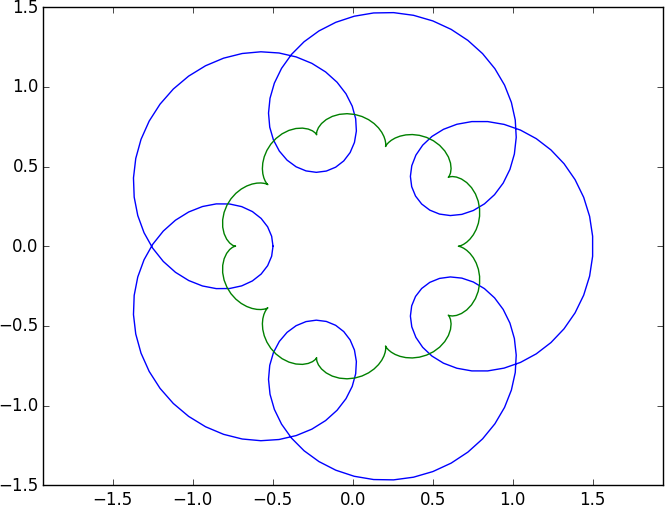
\includegraphics[width=.4\linewidth]{programmes/Exercice_12/figure_1}
\end{center}

\begin{corrige}
$\quad$
\begin{python}
# Question 4
# ==========
def fonc_d(t):
    xp,yp = fonc_v(t)
    xpp,ypp = fonc_a(t)
    return (xp**2 + yp**2)/(xp*ypp-yp*xpp)
def fonc_c(t):
    fd = fonc_d(t)
    x,y = fonc_p(t)
    xp,yp = fonc_v(t)
    return [x-fd*yp,y+fd*xp]
\end{python}
\end{corrige}

\begin{corrige}
$\quad$
\begin{python}
# Question 5
# ==========
les_xc  = []
les_yc  = []
c = fonc_c(L)
#plt.plot(c[0],c[1])
\end{python}
\end{corrige}

\begin{corrige}
$\quad$
\begin{python}
# Question 6
# ==========
from math import sqrt
def distance(p):
    """
    Calcule la longueur du profil p.
    Entrée : 
     * p(lst) : liste [les_x,les_y]
    Sortie : 
     * L(flt) : longueur du profil.
    """
    L=0
    for i in range(len(p[0])-1):
        x0 = p[0][i]
        y0 = p[1][i]
        x1 = p[0][i+1]
        y1 = p[1][i+1]
        L = L+ sqrt((x1-x0)**2+(y1-y0)**2)
    return L
\end{python}
\end{corrige}

\begin{corrige}
$\quad$
\begin{python}
les_dt = []
les_dist = []
for i in range(10,2000,1) :
    dt = 2*np.pi/i
    L=np.linspace(-np.pi,np.pi,i)
    p = fonc_p(L)
    d = distance(p)
    les_dt.append(dt)
    les_dist.append(d)
plt.plot(les_dt,les_dist)
plt.show()       
\end{python}
\end{corrige}


\begin{center}
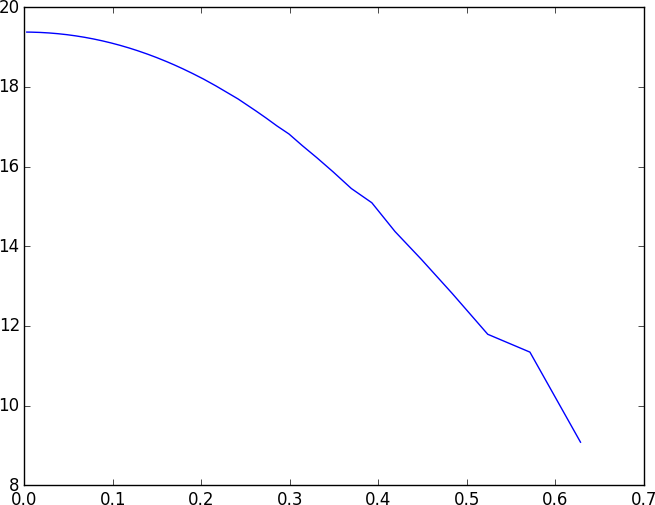
\includegraphics[width=.4\linewidth]{programmes/Exercice_12/figure_2}

\textit{Évolution de la longueur du polynôme en fonction de $\delta t$.}
\end{center}


%\end{multicols}

\newpage 

\section{Correction -- Adaptés des exercices de F. Butin}

\begin{multicols}{2}
%\addcontentsline{toc}{subsection}{Exercice 10 -- Corrigé}
\subsection*{Exercice 10 -- Corrigé}
\textit{D'après Lucie Bathie, PT$\star$ 2015--2016.}


\begin{corrige}
$\quad$
\begin{python}
##Exo 10: palindrome
#1.
def inverse(mot):
    """renvoie la chaine de caractères écrite à l'envers"""
    liste = []
    for k in range(len(mot)):
        liste.append(mot[k])
    inverse = ''
    for i in range(1,len(liste)+1):
        inverse = inverse + liste[-i]
    return(inverse)
#print(inverse('bonjour'))
#ruojnob
\end{python}
\end{corrige}

\begin{corrige}
$\quad$
\begin{python}
#2.
def palindrome(mot):
    return(inverse(mot)==mot)
#print(palindrome('kayak'))
#True
#print(palindrome('bonjour'))
#False
\end{python}
\end{corrige}


\begin{corrige}
$\quad$
\begin{python}
#3.
def pat_nombre(N):
    """renvoie la liste de palindromes 
    inférieurs ou égaux à N"""
    L =[]
    for n in range(N+1):
        if palindrome(str(n)) == True:
            L.append(n)
    return(L)

#print(pat_nombre(100))
#[0, 1, 2, 3, 4, 5, 6, 7, 8, 9, 11, 22, 
#   33, 44, 55, 66, 77, 88, 99]
\end{python}
\end{corrige}


\end{multicols}


%\addcontentsline{toc}{subsection}{Exercice 12 -- Corrigé}
\subsection*{Exercice 12 -- Corrigé}
\textit{D'après Lucie Bathie, PT$\star$ 2015--2016.}

\begin{multicols}{2}

\begin{corrige}
$\quad$
\begin{python}
#1.
v = [1,2,0,4,7,0,0,0,0]

def creux(v):
    """renvoie True si le vecteur est creux, 
    false sinon"""
    nombre_zeros = 0
    for k in range(len(v)):
        if v[k] == 0:
            nombre_zeros +=1
    return(nombre_zeros >= (len(v)-nombre_zeros)/2)

#print(creux(v))
#True
\end{python}
\end{corrige}

\begin{corrige}
$\quad$
\begin{python}
#2.
def coder(v):
    code = [len(v)]
    indices = []
    valeurs = []
    for k in range(len(v)):
        if v[k] != 0:
            indices.append(k)
            valeurs.append(v[k])
    code.append(valeurs)
    code.append(indices)
    return(code)
    
#print(coder(v))
#[9, [1, 2, 4, 7], [0, 1, 3, 4]]    
\end{python}
\end{corrige}

\begin{corrige}
$\quad$
\begin{python}
#3. 
def decoder(code):
    """permet de décoder un codage creux"""
    v=[0]*code[0]
    for k in range(len(code[2])):
        v[code[2][k]] = code[1][k]
    return(v)

code1=[9,[1,2,4,7],[0,1,3,4]]
##print(decoder(code1))
##[1,
\end{python}
\end{corrige}

\begin{corrige}
$\quad$
\begin{python}
#4.
def simul(C,a):
    """C  codage de v
renvoie le codage de av"""
    v = decoder (C)
    for k in range(len(v)):
        v[k] = a*v[k]
    return(coder(v))

#print(simul(code1,2))
#[9, [2, 4, 8, 14], [0, 1, 3, 4]]
\end{python}
\end{corrige}

\begin{corrige}
$\quad$
\begin{python}
#5
def coefficient(j,C):
    vecteur = decoder(C)
    return(vecteur[j])

#print(coefficient(1,code1))
#2
\end{python}
\end{corrige}

\end{multicols}
\newpage
\section{Correction -- Adaptés des exercices de F. Butin}
%\addcontentsline{toc}{subsection}{Exercice 1 -- Corrigé}
\subsection*{Exercice 1 -- Corrigé}
\begin{corrige}
$\quad$
\begin{python}
# Question 1 
# ==========
def affiche_poly(P):
    """
    Affiche un polynome sous la forme 
    a0*X^0+a1*X^1+a2*X^2+...
    Entrée : 
     * P(lst) : liste des coefficients du polynome 
       [a0,a1,...,an]
    Sortie : 
     * Rien. Affichage
    """
    ch=""
    for i in range(len(P)):
        signe="+"
        if P[i]<0 :
            signe="-"
        
        ch=ch+signe+str(abs(P[i]))+"*X^"+str(i)
    print(ch)
\end{python}
\end{corrige}

\begin{corrige}
$\quad$
\begin{python}
# Question 2
# ==========
def degre_poly(P):
    """
    Calcule le degré d'un polynome.
    On se base uniquement sur la taille de la liste 
    à cause de la comparaison à zero
    Entrée : 
     * P(lst) : liste des coefficients du polynome 
       [a0,a1,...,an]
    Sortie : 
     * deg(int) : dege du polynome
    """
    return len(P)-1
\end{python}
\end{corrige}

\begin{corrige}
$\quad$
\begin{python}
# Question 3
# ==========
def add_poly(P1,P2):
    """
    Calcule la somme de deux polynomes.
    Attention à bien faire une copie...
    Entrée : 
     * P1, P2(lst) : liste des coefficients du 
        polynome [a0,a1,...,an]
    Sortie : 
     * P(lst) : liste des coefficients du 
        polynome [a0+b0,a1+b1,...,an+bn]
    """
    # On cherche le polynome le plus grand
    if degre_poly(P1)>=degre_poly(P2):
        P=P1.copy()
        for i in range(len(P2)):
            P[i]=P[i]+P2[i]
    else :
        P=P2.copy()
        for i in range(len(P1)):
            P[i]=P[i]+P1[i]
    return P
\end{python}
\end{corrige}

\begin{corrige}
$\quad$
\begin{python}
def mul_poly(P1,P2):
    """
    Calcule la multiplication de deux polynomes.
    Entrée : 
     * P1, P2(lst) : liste des coefficients du 
       polynome [a0,a1,...,an]
    Sortie : 
     * P(lst) : produits des polynomes
    """
    P=[0]*(degre_poly(P1)+degre_poly(P2)+1)
    for i in range(len(P1)):
        for j in range(len(P2)):
           P[i+j] = P[i+j]+ P1[i]*P2[j]
    return P
\end{python}
\end{corrige}

\begin{corrige}
$\quad$
\begin{python}
def mul_poly(P1,P2):
    """
    Calcule la multiplication de deux polynomes.
    Entrée : 
     * P1, P2(lst) : liste des coefficients du 
        polynome [a0,a1,...,an]
    Sortie : 
     * P(lst) : produits des polynomes
    """
    P=[0]*(degre_poly(P1)+degre_poly(P2)+1)
    for i in range(len(P1)):
        for j in range(len(P2)):
           P[i+j] = P[i+j]+ P1[i]*P2[j]
    return P
\end{python}
\end{corrige}



\begin{corrige}
$\quad$
\begin{python}
# Question 4
# ==========
def prsc_poly(P1,P2):
    """
    Calcule le produit scalaire de deux polynomes.
    Attention à bien faire une copie...
    Entrée : 
     * P1, P2(lst) : liste des coefficients du 
       polynome [a0,a1,...,an]
    Sortie : 
     * P(flt) :produit des coefficients des 
        polynomes a0*b0+a1*b1+...
    """
     # On cherche le polynome le plus grand
    if degre_poly(P1)>=degre_poly(P2):
        P=P1.copy()
        for i in range(len(P2)):
            P[i]=P[i]*P2[i]
    else :
        P=P2.copy()
        for i in range(len(P1)):
            P[i]=P[i]*P1[i]
    return sum(P)
\end{python}
\end{corrige}

\begin{corrige}
$\quad$
\begin{python}
# Question 5
# ==========
def deriv_poly(P):
    """
    Calcule la dérivée d'un polynome.
    Entrée : 
     * P(lst) : liste des coefficients du 
        polynome [a0,a1,...,an]
    Sortie : 
     * coefficients du polynome dérivé
    """
    return [P[i]*i for i in range(1,len(P))]
\end{python}
\end{corrige}




%\columnbreak
%\addcontentsline{toc}{subsection}{Exercice 3 -- Corrigé}
\subsection*{Exercice 3 -- Corrigé}

\begin{corrige}
$\quad$
\begin{python}
import numpy as np
import matplotlib.pyplot as plt
# Question 1 
# ==========
def f_sigma(n,t):
    return (np.cos(n*t))**3-(np.sin(n*t))**3

x = np.linspace(0,10,1000)
y = f_sigma(1,x)

for i in range(4):
    x = np.linspace(0,10,1000)
    y = f_sigma(i,x)
    plt.plot(y*np.cos(x),y*np.sin(x),label=str(i))

plt.legend()
plt.axis("equal")    
plt.show()
\end{python}
\end{corrige}
\begin{center}
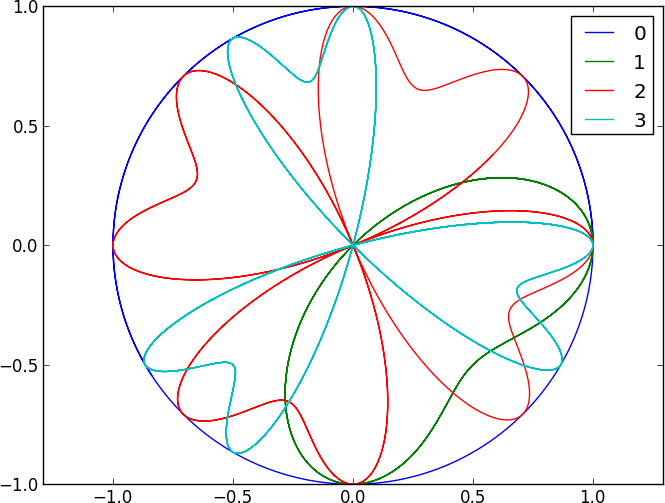
\includegraphics[width=.4\linewidth]{images/exo_FB_03}
\end{center}

%\columnbreak
%\addcontentsline{toc}{subsection}{Exercice 7 -- Corrigé}
\subsection*{Exercice 7 -- Corrigé}

\begin{corrige}
$\quad$
\begin{python}
# Question 2
# ==========
R=4
r=R/4
m = 1-R/r
theta = np.linspace(0,2*np.pi,1000)
x=(R-r)*np.cos(theta)+r*np.cos(m*theta)
y=(R-r)*np.sin(theta)+r*np.sin(m*theta)
plt.plot(x,y,label="R=4, r=1, m=-3")
\end{python}
\end{corrige}

\begin{center}
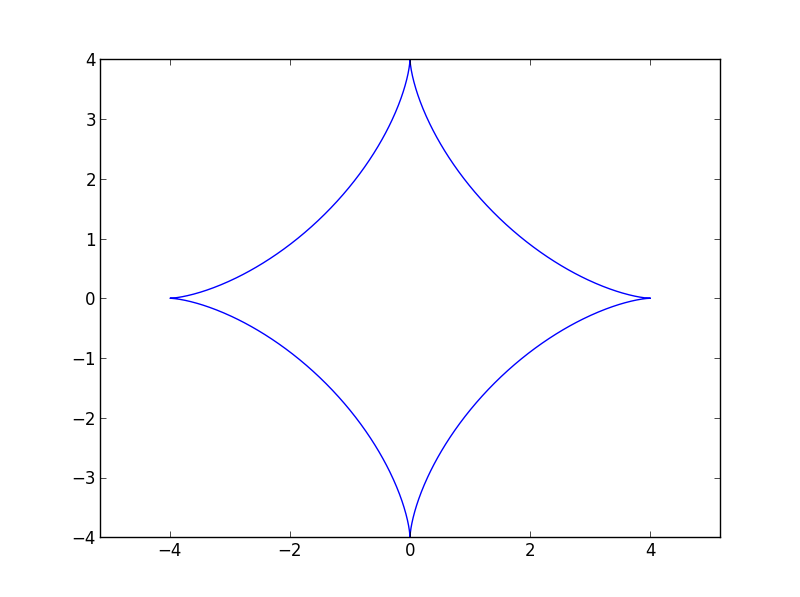
\includegraphics[width=.4\linewidth]{images/exo_FB_07_1}
\end{center}

\begin{corrige}
$\quad$
\begin{python}
# Question 3
# ==========
for p in [1, 5, 10, 100]:
    r=R/p
    m = 1-R/r
    theta = np.linspace(0,2*np.pi,1000)
    x=(R-r)*np.cos(theta)+r*np.cos(m*theta)
    y=(R-r)*np.sin(theta)+r*np.sin(m*theta)
    titre = "R="+str(R)+", r = "+str(r)+ ",m="+str(m)
    plt.plot(x,y,label=titre)

x=R*np.cos(m*theta)
y=R*np.sin(m*theta)
#plt.plot(x,y)

plt.axis("equal")
#plt.legend()
plt.show()
\end{python}
\end{corrige}

\begin{center}
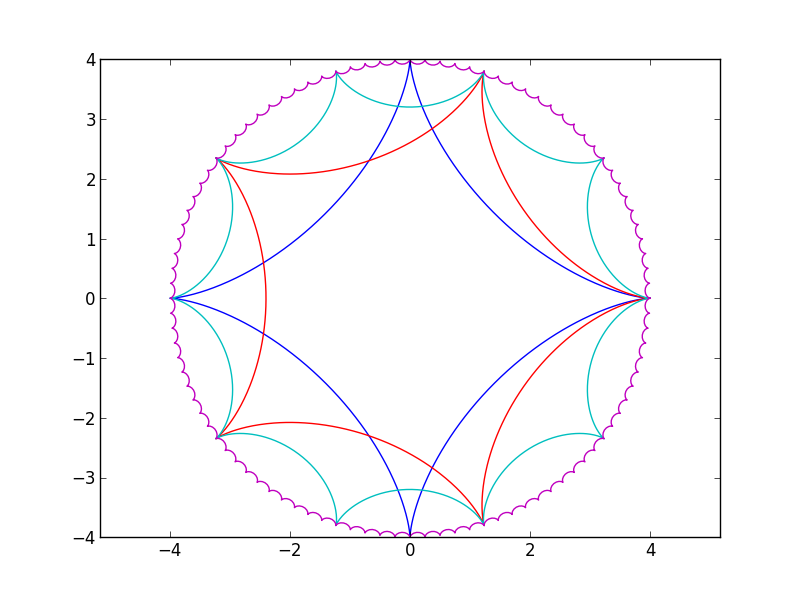
\includegraphics[width=.4\linewidth]{images/exo_FB_07_2}
\end{center}




%\columnbreak 
%\addcontentsline{toc}{subsection}{Exercice 9 -- Corrigé}
\subsection*{Exercice 9 -- Corrigé}

\begin{corrige}
$\quad$
\begin{python}
# EXERCICE 9
import numpy as np
import matplotlib.pyplot as plt
import turtle

# Question 1 
#============
turtle.hideturtle()
turtle.goto(100,0)
turtle.speed(1)
tortue = turtle.Pen()

t = np.linspace(0,2*np.pi,1000)
x=100*np.cos(t)
y=100*np.sin(t)
for i in range(len(x)):
    tortue.goto(x[i],y[i])
\end{python}
\end{corrige}


\begin{center}
\begin{tabular}{cc}
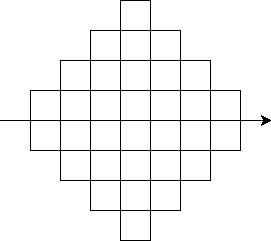
\includegraphics[width=.3\linewidth]{images/exo_FB_09_01}&
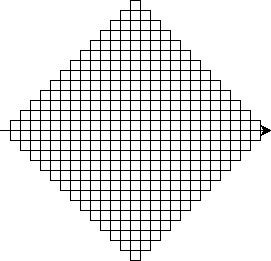
\includegraphics[width=.3\linewidth]{images/exo_FB_09_02}
\end{tabular}
\end{center}



\begin{corrige}
$\quad$
\begin{python}
# Question 2 
# ==========
def peano(n) : 
    if n==1 :
        tortue.forward(10)
    else : 
        peano(n-1)
        tortue.left(90)
        peano(n-1)
        tortue.left(-90)
        peano(n-1)
        tortue.left(-90)
        peano(n-1)
        tortue.left(-90)
        peano(n-1)
        tortue.left(90)
        peano(n-1)
        tortue.left(90)
        peano(n-1)
        tortue.left(90)
        peano(n-1)
        tortue.left(-90)
        peano(n-1)
        
peano(4)
turtle.hideturtle()
\end{python}
\end{corrige}


%\columnbreak 

%\addcontentsline{toc}{subsection}{Exercice 10 -- Corrigé}
\subsection*{Exercice 10 -- Corrigé}


\begin{corrige}
$\quad$
\begin{python}
# EXERCICE 10 FB
import numpy as np
import matplotlib.pyplot as plt
import turtle
__author__ = "Frederic Butin"

# Question 1 
# ==========
turtle.hideturtle()
turtle.speed(10);
tortue = turtle.Pen()

def koch (n):
    if n==1 : 
        tortue.forward(3)
    else : 
        koch(n-1);
        tortue.left(60)
        koch(n-1);
        tortue.left(-120)
        koch(n-1);
        tortue.left(60)
        koch(n-1)
        

def flocon(n):
    tortue.clear()
    koch(n)
    tortue.left(-120)
    koch(n)
    tortue.left(-120)
    koch(n)
    tortue.hideturtle()

flocon(5)
\end{python}
\end{corrige}



%\addcontentsline{toc}{subsection}{Exercice 11 -- Corrigé}
\subsection*{Exercice 11 -- Corrigé}

\begin{corrige}
$\quad$
\begin{python}
# EXERCICE 11
# Question 1 
# ==========
import matplotlib.pyplot as plt
import math

I_th = 8*math.log(2)-3
\end{python}
\end{corrige}

\begin{corrige}
$\quad$
\begin{python}
# Question 2
# ==========
def fonc(x):
    return math.log(x)
\end{python}
\end{corrige}


\begin{corrige}
$\quad$
\begin{python}    
def calc_int_trap(a,b,n):
    res = 0
    pas = (b-a)/n
    x = a+pas
    i=1
    while i<n:
        res = res + fonc(x)
        x = x + pas
        i=i+1
    res = pas*(res+(fonc(a)+fonc(b))/2)
    return res
\end{python}
\end{corrige}


\begin{corrige}
$\quad$
\begin{python}    
def calc_int_rect_g(a,b,n):
    res = 0
    pas = (b-a)/n
    x = a
    i=0
    while i<n:
        res = res + fonc(x)
        x = x + pas
        i=i+1
    return res*pas
\end{python}
\end{corrige}


\begin{corrige}
$\quad$
\begin{python}
N = [10,20,40,100,200, 400, 500, 600, 700, 800, 
        900, 1000, 5000, 10000, 20000, 100000]

calc_int_trap(1,4,10)
err_trap = [abs(I_th-calc_int_trap(1,4,n)) 
                                           for n in N]
err_rect = [abs(I_th-calc_int_rect_g(1,4,n)) 
                                           for n in N]

plt.loglog(N,err_trap,label = "Erreur trapèze")
plt.loglog(N,err_rect,label = "Erreur rectangle")
plt.legend()
plt.grid()
plt.show()

\end{python}
\end{corrige}

\begin{center}
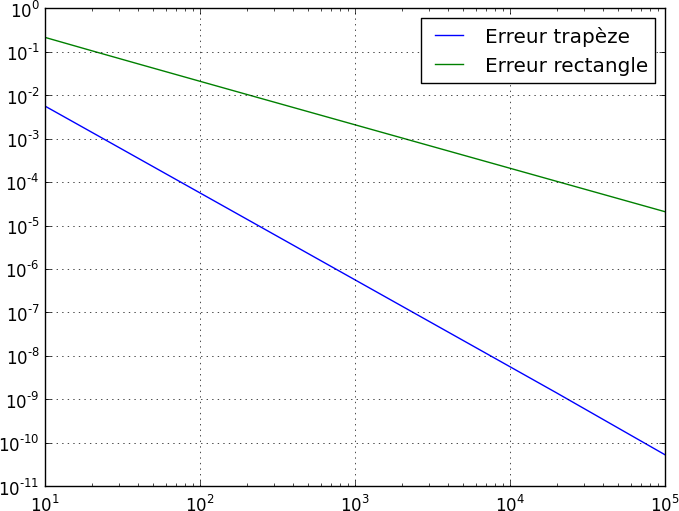
\includegraphics[width=.4\linewidth]{images/exo_FB_11}
\end{center}


%\columnbreak

%\addcontentsline{toc}{subsection}{Exercice 12 -- Corrigé}
\subsection*{Exercice 12 -- Corrigé}

\begin{corrige}
\textcolor{red}{A refaire ?}


On pose : 
$$\left\{
\begin{array}{l}
y_1(t) = x(t) \\
y_2(t) = x'(t)
\end{array}
\right.
$$

En utilisant le schéma d'Euler explicite, on a :
$$\left\{
\begin{array}{l}
y'_1(k)=\dfrac{y_1(k+1)-y_1(k)}{h} \\
y'_2(k)=\dfrac{y_2(k+1)-y_2(k)}{h}
\end{array}
\right.
$$

On a donc : 
$$\left\{
\begin{array}{l}
y'_1(t)=y_2(t) \\
y'_2(t)+10y_2(t) - y_1(t) = \sin \left(nt\right)
\end{array}
\right.
$$

En discrétisant l'équation on a donc : 
$$\left\{
\begin{array}{l}
y_2(k) =\dfrac{y_1(k+1)-y_1(k)}{h} \\
\dfrac{y_2(k+1)-y_2(k)}{h} +10y_2(k) - y_1(k) = \sin \left(nk\right)
\end{array}
\right.
$$

$$\Leftrightarrow
\left\{
\begin{array}{l}
y_1(k+1) = hy_2(k)+y_1(k) \\
y_2(k+1)  = h \left(  \sin \left(nk\right)+ y_1(k)-10y_2(k) \right)+y_2(k)
\end{array}
\right.
$$

\end{corrige}

\begin{corrige}
Mise en forme matricielle du problème : 
On pose : 
$$
X = \left[
\begin{array}{c}
x(t) \\
x'(t)
\end{array}
\right]
\Rightarrow
X' = \left[
\begin{array}{c}
x'(t) \\
x''(t)
\end{array}
\right]
$$

On a alors : $$
\left[
\begin{array}{c}
x'(t) \\
x''(t)
\end{array}
\right]
=
 \left[
\begin{array}{cc}
0 & 1 \\
 1 &- 10\\
\end{array}
\right]
\cdot
 \left[
\begin{array}{c}
x(t) \\
x'(t)
\end{array}
\right]
+
\left[
\begin{array}{c}
0 \\
\sin (nt)
\end{array}
\right]
$$

Le système peut donc se mettre sous la forme : 
$$
X'(t) = AX(t)+ B(t)
$$

En appliquant un schéma d'Euler explicite, on a donc :
$$
X'(t) \simeq \dfrac{X_{k+1}-X_{k}}{h}
$$ 

D'où :

$$
\dfrac{X_{k+1}-X_{k}}{h} = AX_k + B_k 
\Leftrightarrow 
X_{k+1} = (hA +1) X_k + hB_k
$$
\end{corrige}

%%\columnbreak


\begin{corrige}
Mise en forme du problème de Cauchy : 

En réutilisant la mise en forme matricielle précédente, on peut donc définit la fonction $f$ telle que : 
$$
f(X,t) \mapsto  AX(t) + B(t)
$$


\begin{python}
import matplotlib.pyplot as plt
import numpy as np
import scipy.integrate as spi
N=10000

def fonction_f(X,t,n):
   return [X[1],X[0]-10*X[1]+np.sin(n*t)]

les_t=np.linspace(0,7,N)
for i in range(0,11):
    res = spi.odeint(fonction_f,[0,1],les_t,(i,))
    plt.plot(les_t,res[:,0])
plt.show()
\end{python}
\end{corrige}

\begin{center}
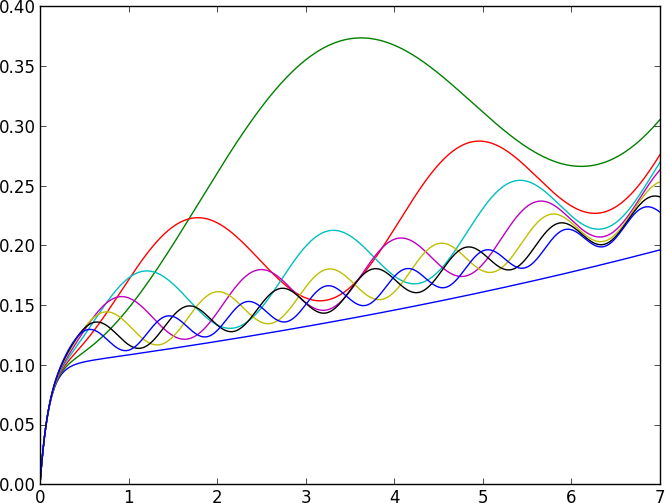
\includegraphics[width=.4\linewidth]{images/exo_FB_12}
\end{center}


%\columnbreak
%\addcontentsline{toc}{subsection}{Exercice 13 -- Corrigé en cours}
\subsection*{Exercice 13 -- Corrigé}

\begin{corrige}
On pose : 
$$
X_i =\begin{bmatrix}
F_{i+1} \\
F_{i}
\end{bmatrix} 
$$

Le problème peut être mis sous la forme matricielle suivante : 
$$
X_{i+1} =
\begin{bmatrix}
F_{i+2} \\
F_{i+1}
\end{bmatrix} 
=
\begin{bmatrix}
1 & 1  \\
1 & 0 
\end{bmatrix} 
\begin{bmatrix}
F_{i+1} \\
F_{i}
\end{bmatrix} 
\Leftrightarrow X_{i+1} = M X_{i}
$$

On  peut donc écrire que  :
$$
X_{i+1} =
\begin{bmatrix}
1 & 1  \\
1 & 0 
\end{bmatrix} 
\begin{bmatrix}
F_{i+1} \\
F_{i}
\end{bmatrix} 
=
\begin{bmatrix}
1 & 1  \\
1 & 0 
\end{bmatrix} 
\begin{bmatrix}
1 & 1  \\
1 & 0 
\end{bmatrix} 
\begin{bmatrix}
F_{i} \\
F_{i-1}
\end{bmatrix} 
$$
 On a donc :
 $$
X_{n} = M^n X_{0}
$$

\end{corrige}



%\addcontentsline{toc}{subsection}{Exercice 19}
\subsection*{Exercice 19}

\begin{corrige}
$\quad$
\begin{python}
# EXERCICE 19
# Question 1 
# ==========
import numpy as np
import scipy.integrate as sci
import matplotlib.pyplot as plt

def fonction_PP(X,t,a,b,c,d):
    return [a*X[0]-b*X[0]*X[1],-c*X[1]+d*X[0]*X[1]]

def fonction_PP2(X,t):
    a,b,c,d = 1,1,1,1
    return [a*X[0]-b*X[0]*X[1],-c*X[1]+d*X[0]*X[1]]
\end{python}
\end{corrige}


\begin{corrige}
$\quad$
\begin{python}
# Question 2 
# ==========
# Conditions initiale : 
X0=[1,2]
t = np.linspace(0,20,1000)
res = sci.odeint(fonction_PP2,X0,t)
\end{python}
\end{corrige}

\begin{corrige}
$\quad$
\begin{python}
# Question 3 
# ==========
plt.figure()
plt.plot(t,res[:,0])
plt.plot(t,res[:,1])
\end{python}
\end{corrige}

\begin{corrige}
$\quad$
\begin{python}
# Question 4 
# ==========
plt.figure()
plt.plot(res[:,0],res[:,1])
plt.axis("equal")
\end{python}
\end{corrige}



\begin{center}
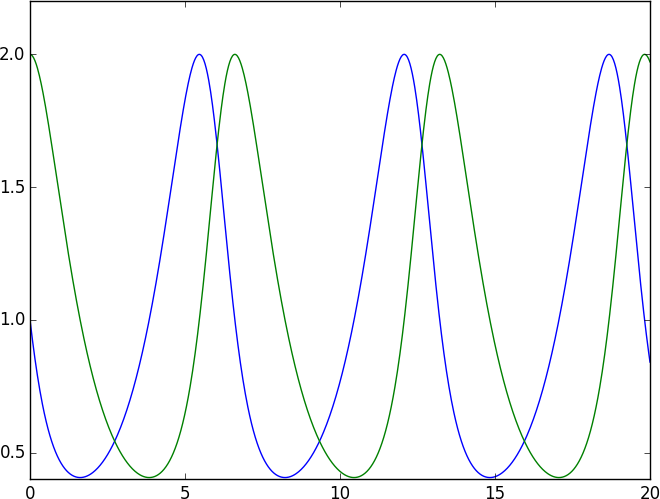
\includegraphics[width=.45\linewidth]{exo_fb_19_01.png}
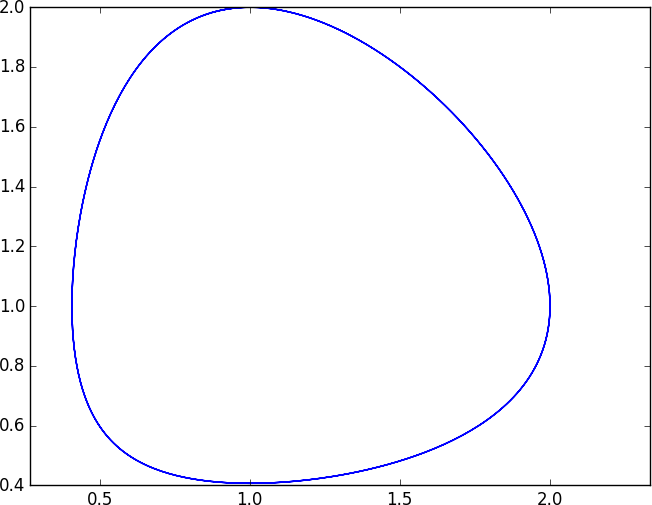
\includegraphics[width=.45\linewidth]{exo_fb_19_02.png}
\end{center}
%\end{multicols}

%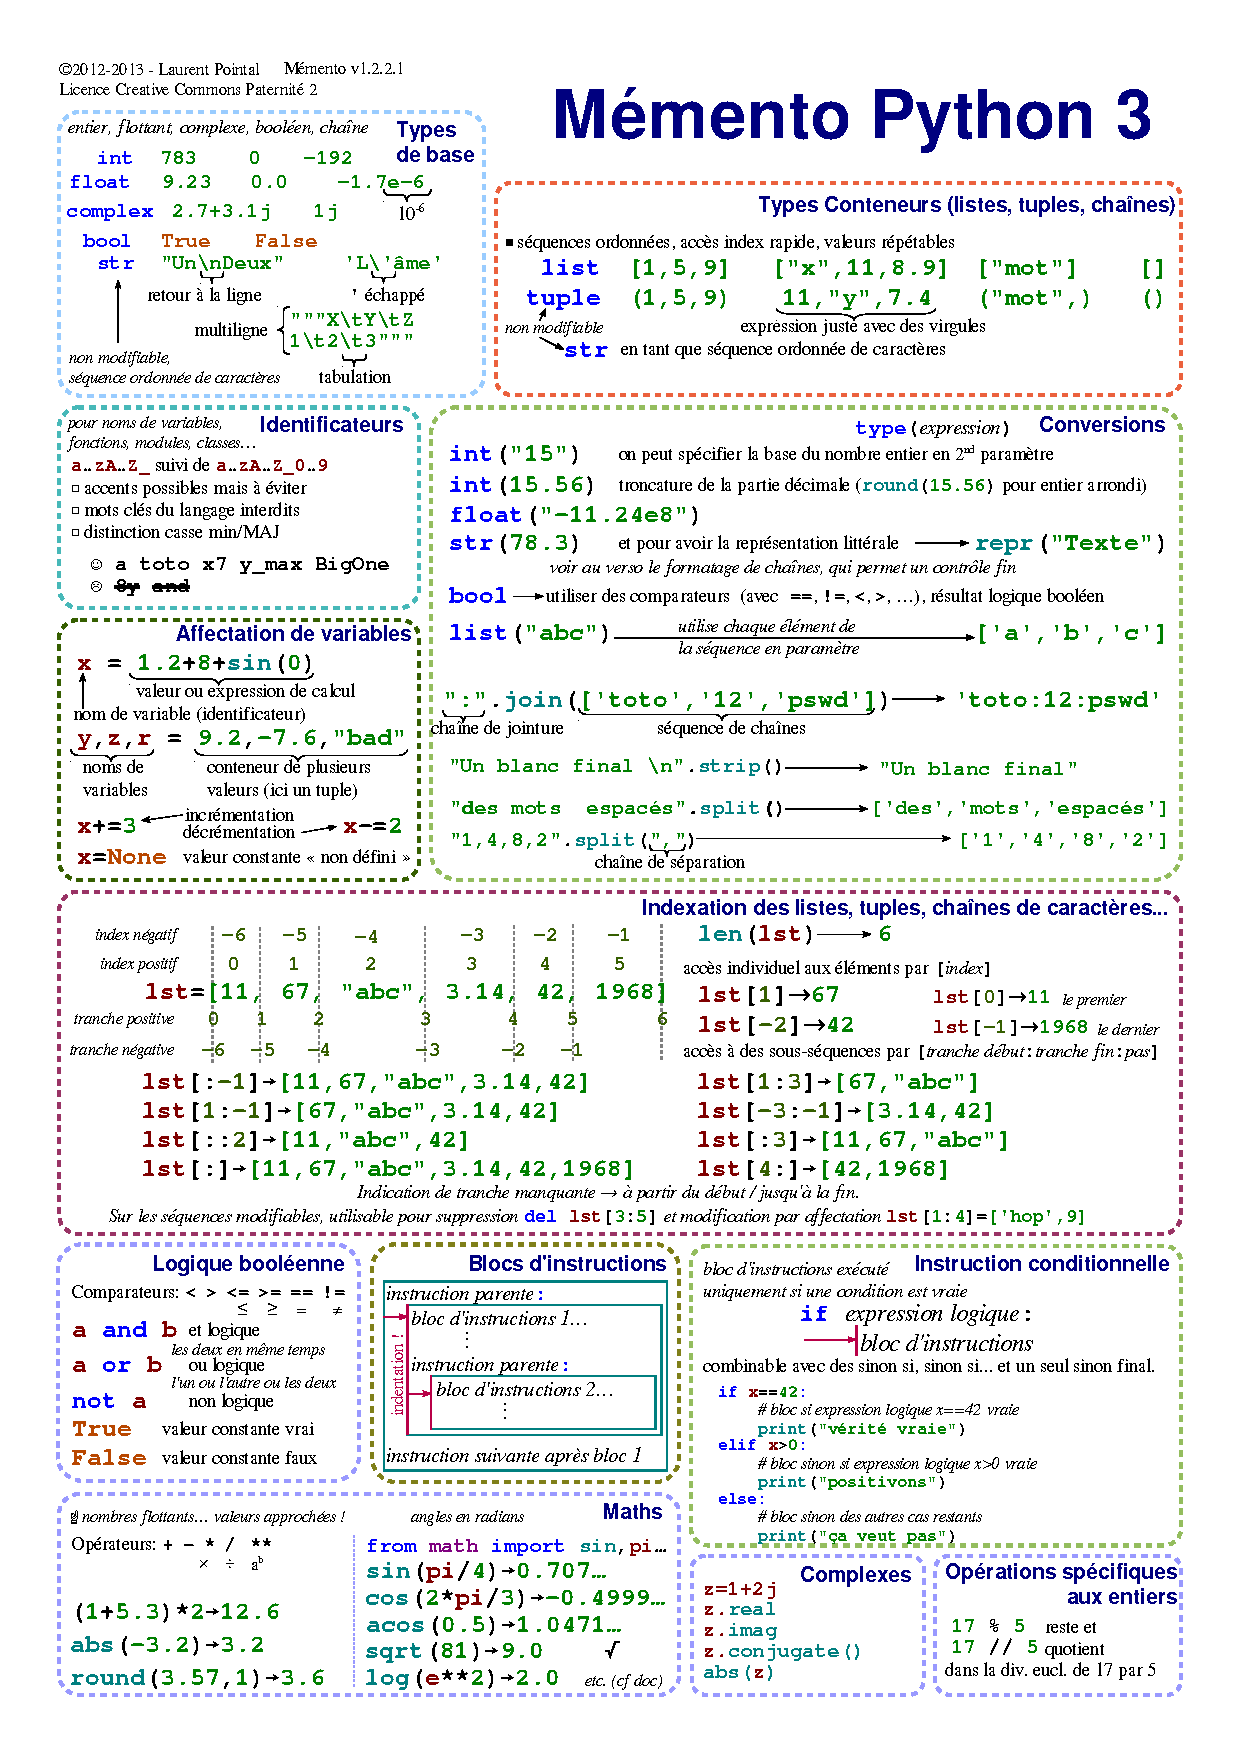
\includepdf[pages={1-4},]{images/MementoPythonScilab}

\newpage 
\section{Exercices de la Banque PT -- 2016}
\subsection*{Exercice 1  -- \ding{51}}
\begin{corrige}
$\quad$
\begin{python}
import math as m
# EXERCICE 2016 01
def suite (n,nb):
    i=1
    res=nb
    while n > 0:
        res = (res+module(res))/2
       # print(i,res)
        n=n-1
        i+=1
    return res


def module(nb):
    return(m.sqrt(nb.real**2+nb.imag**2))

def suite2(nb):
    i=1
    res=nb
    while abs(res.imag)>0.01:
        res = (res+module(res))/2
        i=i+1
    return i

print(suite(12,1+10j))
print(suite2(1+10j))
\end{python}
\end{corrige}


\subsection*{Exercice 2}
\textit{D'après Léo Chabert, PT$\star$ 2016 -- 2017.}
\begin{corrige}
$\quad$
\begin{python}
import numpy as np

#Q1
def produit(L,C):
    """ Renvoie le produit de la ligne L par la colonne C """
    l = np.array(L)
    c = np.array(C)

    return(np.dot(L,C))
    
L1 = [[1,-1]]
C1 = [[1],[1]]

#print(produit(L1,C1))
#[[0]]

#Q2

def ligne(M,i) :
    """ Renvoie le vecteur de la ligne i de M,
    M sous la forme d'une liste simple"""
    n = len(M)
    j = int(np.sqrt(n))

    return (M[(i-1)*j : i*j])

M = [1,1,1,1,1,0,1,0,0]
#print(ligne(M,2))
#[1, 1, 0]

#Q3

def colonne(M,j) :
    """ Renvoie le vecteur de la colonne j de M,
    M sous la forme d'une liste simple"""
    n = len(M)
    i = int(np.sqrt(n))

    return([M[(a*i)+(j-1)] for a in range(i)])

#print(colonne(M,3))
#[1, 0, 0]

#Q4

def produit_mat(M,N) :
    """ Effectue le produit matriciel de M par N, deux matrices sous forme de liste """
    P =[]
    n = int(np.sqrt(len(M)))

    for i in range(1,n+1):
        for j in range(1,n+1):
            L = ligne(M,i)
            C = colonne(N,j)
            
            P.append(produit(L,C))
    return(P)

N = [1,0,0,0,1,0,0,0,1]

#print(produit_mat(M,N))
#[1, 1, 1, 1, 1, 0, 1, 0, 0]      
\end{python}
\end{corrige}

\subsection*{Exercice 3}
\textit{D'après Léo Chabert, PT$\star$ 2016 -- 2017.}
\begin{corrige}
$\quad$
\begin{python}
import random as r
import numpy as np
import matplotlib.pyplot as plt

#Q1
 #Modification du programme (il manque l'initialisation )

def ordonner(L):
    if len(L) == 0 :
        return([])
    if len == 1 :
        return(L)
    if len(L) == 2 :
        if L[1]<=L[0] :
            return(L)
        else :
            return([L[1],L[0]])
    if len(L) >= 3 :
        n = 1
        e0 = L[0]
        Linf,Lsup = [],[]
        for ei in L[1:]:
          if ei == e0 :
              n+= 1
          elif ei < e0  :
              Linf.append(ei)
          else :
              Lsup.append(ei)

        return(ordonner(Linf)+ n *[e0] + ordonner (Lsup))

#Ordonner permet de classer la liste L par ordre croissant

#Q2

def less(z1,z2):
    """ Renvoie True si Re(z1)<Re(z2) ou (Re(z1)=Re(z2) et Im(z1) < Im (z2) """
    B = (((z1.real) < (z2.real)) or ((z1.real) == (z2.real) and (z1.imag < z2.imag)))

    return(B)

#print(less(1+2j,1+3j))
#True

#Q3

def ordonnerdansc(L):
    """ Ordonner la liste L d'après la méthode de la liste ordonner, 
    en s'appuyant sur l'ordonnancement de la fonction less """
    if len(L) == 0 :
        return([])
    if len(L) == 1 :
        return(L)
    if len(L) == 2 :
         if less(L[1],L[0]) :
             return(L)
         else :
             return([L[1],L[0]])
    if len(L) >= 3 :
        n = 1
        e0 = L[0]
        Linf,Lsup = [],[]
        for ei in L[1:]:
             if ei == e0 :
                 n+= 1
             elif less(ei,e0) :
                 Linf.append(ei)
             else :
                 Lsup.append(ei)
        
        return(ordonnerdansc(Linf) + n *[e0] + ordonnerdansc(Lsup))
    
#Q3
L = []
for i in range(11):
    a = r.randint(-10,10)
    b = r.randint(-10,10)
    L.append(a+b*1j)


#print (L)
#print(ordonnerdansc(L))

#[(-3-5j), (-2+0j), (9-6j), (4+1j), (-2+2j), (2-1j), (2-4j), (-5-1j), (3+9j), (-5+6j), (-7-9j)]
#[(-7-9j), (-5-1j), (-5+6j), (-3-5j), (-2+0j), (-2+2j), (2-4j), (2-1j), (3+9j), (4+1j), (9-6j)]


#Q4

Lpi = []

for a in range(-100,100):
    Lpi.append((20+ np.cos(10*a*np.pi/100))*np.exp((a*np.pi/100)*1j))

Lpi = ordonnerdansc(Lpi)

Lpir = []
Lpiim =[]

for z in Lpi :
        Lpir.append(z.real)
        Lpiim.append(z.imag)
        
plt.plot(Lpir,Lpiim,'o',label = 'Lpi')

plt.xlabel('Re()')
plt.ylabel('Im()')

plt.legend()
plt.show()
\end{python}
\begin{center}
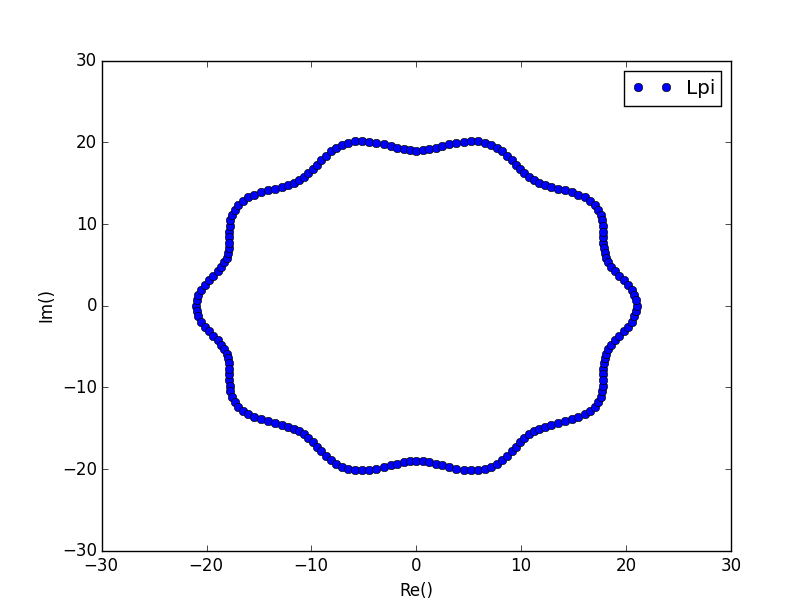
\includegraphics[width=7cm]{programmes/Exercice_2016_03/figure_1}
\end{center}
\end{corrige}

\subsection*{Exercice 4}
\textit{D'après Ayoub Elghaoui, PT$\star$ 2016 -- 2017.}
\begin{corrige}
$\quad$
\begin{python}
#question 1

def dédoublement(L):
    n =len(L)
    k=0
    P=[]
    while k < n :
        v=L[k]
        S=0
        while k<n and L[k] == v:
            S=S+1
            k=k+1
        P.append(S)
        P.append(v)
    return(P)

##print(dédoublement([1,1,1,2,2,2]))
##>>> 
##[3, 1, 3, 2]

#question2

def chaine(P):
    C=str(P[0])
    n=len(P)
    for k in range(1,n):
        C=C+','+str(P[k])
    return(C)

##print(chaine(dédoublement([1,1,1,2,2,2])))
##>>> 
##3,1,3,2

def dédoubl_recurence(L,n):
    for k in range(n):
        L=dédoublement(L)
    return(L)


def dédouble_recursive(L,n):
    if n == 0:
        return(L)
    else:
        L=dédoublement(L)
        return(dédouble_recursive(L,n-1))

##print(dédouble_recursive([1],3))
##print(dédoubl_recurence([1],3))
##>>> 
##[1, 2, 1, 1]
##[1, 2, 1, 1]
\end{python}
\end{corrige}

\subsection*{Exercice 5}
\textit{D'après Ayoub Elghaoui, PT$\star$ 2016 -- 2017.}

\begin{corrige}
$\quad$
\begin{python}
#### Exercice 5
##question 1:
#cette fonction crée une liste de chiffre à partir d'un nombre, les elements de la liste sont les chiffres 
### qui composent le nombre

##question 2:
def chiffres (n):
    L=[]
    for k in range(len(str(n))):
        if n == 0:
            return[0]
        if n != 0:
            L.append(n%10)
            n=n//10
    return(L)

def calcul_narcissique(n):
    p=len(str(n))
    L=chiffres(n)
    S=0
    for k in range (p):
        S=S+L[k]**p 
    return(S)

# print(calcul_narcissique(93084))
# 93084

##question 3:
def verif_narcissique(n):
    return(calcul_narcissique(n)==n)
    
# print(verif_narcissique(93084))
# True

##question 4
l=[]
for k in range(100000):
    if verif_narcissique(k) == True:
        l.append(k)
    
# print(l)
# [0, 1, 2, 3, 4, 5, 6, 7, 8, 9, 153, 370, 371, 407, 1634, 8208, 9474, 54748, 92727, 93084]
\end{python}
\end{corrige}


\subsection*{Exercice 6}
\textit{D'après Ayoub Elghaoui, PT$\star$ 2016 -- 2017.}

\begin{corrige}
$\quad$
\begin{python}
import matplotlib.pyplot as plt
import numpy as np
import random as rdm

####Exercice 6 ####
A=[1,5]
B=[2,8]
C=[7,1]

##question 1:
def triangle(a,b,c):
    plt.plot([a[0],b[0],c[0]],[a[1],b[1],c[1]],'r')
        plt.plot([c[0],a[0]],[c[1],a[1]],'r')

triangle(A,B,C)
plt.show()
##question 2:

def milieu(a,b):
    I=[(a[0]+b[0])/2,(a[1]+b[1])/2]
    return(I)

print(milieu(A,B))

##question 3:

def cal_milieu(p):
    L=[A,B,C]
    a=L[rdm.randint(0,2)]
    I=milieu(a,p)
    
    return(I)

## question 4 :

p=[1,1] # point p choisi arbitrairement

L=[]
for k in range(1000):
    L.append(cal_milieu(p))

les_x=[]
les_y=[]

for l in range(len(L)):
    les_x.append(L[l][0])
    les_y.append(L[l][1])

triangle(A,B,C)
plt.xlim(0,10)
plt.ylim(0,10)
plt.plot([p[0]],[p[1]],'*')
plt.plot(les_x,les_y,'+-g')
plt.show()
\end{python}
\end{corrige}

\subsection*{Exercice 7}
\textit{D'après Léo Chabert, PT$\star$ 2016 -- 2017.}

\begin{corrige}
$\quad$
\begin{python}
##Q1

# 400 Zholty : Impossible !
# 400 divisible par 10 => Si on veut faire avec ces billets, il en faudra 5 ou 10
# Si on en prend 5, on sera en dessous et la valeur à combler sera trop petite, 
# Si on en prend 10 on est forcément au dessus (10*52 > 400 )

##Q2

Billets = [52,62,72]

def somme(p) :
    """ p = [a,b,c], renvoie la somme de a billets de 52 etc... """
    return(p[0]*Billets[0] + p[1]*Billets[1] + p[2]*Billets[2])
    
#print(somme([0,0,0]))
#print(somme([4,2,1]))
#0
#404
    
def compte(n) :
    """ Donne les possibilités pour obtenir n avec des triplets de bilets """
    Poss = []
    a,b,c = 0,0,0
    p = [a,b,c]
    
    while somme(p) < n : 
        #On incrémente d'abord sur le a, après avoir testé toutes les combinaisons pour une valeur de a 
        while somme(p) < n :
            #Id. pour b et c
            
            while somme(p) < n :
                c += 1
                p = [a,b,c]
                
            if somme(p) == n :
                Poss.append(p)
            
            c = 0
            b += 1
            p = [a,b,c]
            
        b = 0
        a += 1
        p = [a,b,c]
    
    return(Poss)
    
#print(compte(600))
#print(compte(400))
#[[3, 6, 1], [4, 4, 2], [5, 2, 3], [6, 0, 4]]
#[]

##Q3

res = []


for i in range(72, 600) :
    #On cherche les possibilités entre 72z et 600z avec 4z d'écarts
    
    if compte(i) != [] :
        if compte(i-4) != []:
            res.append(i)
            

#print(res)
#[436, 488, 498, 508, 540, 550, 560, 570, 580, 592]

for val in res :
    print(compte(val),compte(val-4))
                
                
# [[7, 0, 1]] [[0, 0, 6]]
# [[8, 0, 1]] [[0, 2, 5], [1, 0, 6]]
# [[7, 1, 1]] [[0, 1, 6]]
# [[6, 2, 1], [7, 0, 2]] [[0, 0, 7]]
# [[9, 0, 1]] [[0, 4, 4], [1, 2, 5], [2, 0, 6]]
# [[8, 1, 1]] [[0, 3, 5], [1, 1, 6]]
# [[7, 2, 1], [8, 0, 2]] [[0, 2, 6], [1, 0, 7]]
# [[6, 3, 1], [7, 1, 2]] [[0, 1, 7]]
# [[5, 4, 1], [6, 2, 2], [7, 0, 3]] [[0, 0, 8]]
# [[10, 0, 1]] [[0, 6, 3], [1, 4, 4], [2, 2, 5], [3, 0, 6]]
#A chaque fois, on à au moins deux billets différents
#Il faudrait éventuellement éliminer les cas incohérent  ou l'enfant récupère des billets qu'il avait déjà
\end{python}
\end{corrige}


\subsection*{Exercice 8}
\textit{D'après Léo Chabert, PT$\star$ 2016 -- 2017.}

\begin{corrige}
$\quad$
\begin{python}
import random as r

##Q1
def lancer():
    """ Simule un lancer de dés """
    return(r.randint(1,6))
    
#print(lancer())
#1
    
##Q2
def liste(n) :
    """ Renvoie une liste pour le lancer de n dés """
    return([lancer() for i in range(n)])
    
#print(liste(10)); [5, 3, 3, 2, 4, 6, 4, 5, 1, 1]
L = [5, 3, 3, 2, 4, 6, 4, 5, 1, 1]

##Q3
def arrivee(k,L) :
    """ Simule l'avancée comme proposé """   
    c = k    
    while c < len(L) and c + L[c] < len(L) :
        c += L[k]       
    return(c)
    
#print(arrivee(2,L)) ,5

L_15 = liste(15)
L_20 = liste(20)
L_25 = liste(25)
La_15 = []
La_20 = []
La_25 = []

for k in range (len(L_15)) :
    La_15.append(arrivee(k,L_15))

#print(La_15),[12, 15, 12, 15, 12, 15, 12, 15, 18, 17, 12, 14, 12, 14, 14]

for k in range (len(L_20)) :
    La_20.append(arrivee(k,L_20))

#print(La_20),[18, 19, 20, 17, 18, 20, 18, 17, 18, 18, 19, 17, 17, 17, 17, 17, 17, 17, 18, 19]

for k in range (len(L_25)) :
    La_25.append(arrivee(k,L_25))

"""print(La_25),[24, 25, 22, 21, 21, 25, 24, 23, 22, 21, 22, 21, 22, 23, 22, 
21, 21, 21, 21, 21, 22, 21, 22, 23, 24]"""

##Q4
def commun(L) :
    """ renvoie le plus grand entier tel que l'arrivee de 0,1,2,k soit le même """
    a,b,c = arrivee(0,L),arrivee(1,L),arrivee(2,L)
    k = 0
    res = True
    
    while res and k < len(L) :
        if arrivee(k,L) == a and arrivee(k,L) == b and arrivee(k,L) == c :
            k +=1
        else :
            res = False
        
    return(k-1)
        
#print(commun([6,5,4,3,2,1,1]))
#6
\end{python}
\end{corrige}

\subsection*{Exercice 9}
\textit{D'après Léo Chabert, PT$\star$ 2016 -- 2017.}
\begin{corrige}
$\quad$
\begin{python}
import matplotlib.pyplot as plt
import numpy as np

## Q1

def g(x) :
    """ renvoie la valeur de g(x) """
    return(1)
    
def f(x) :
    """ renvoie la valeur de f(x) """
    
    if x>= 0 and x<1 :
        return(g(x))
    elif x>1 :
        return(x*f(x-1))
    
def H(x) :
    """ prolongement de f(x) à ]-1,0] """
    if x >= 0 :
        return(f(x))
    elif x > -1 :
        return(f(-x))
    
## Q3

les_x = np.arange(-0.99,4.01,0.01)
les_y = []

for x in les_x :
 les_y.append(H(x))

plt.plot(les_x,les_y, 'b',label = 'H(x)')

## Q4

#On approxime la dérivée avec Euler :
# yi' = (yi+1-yi)/dx


def derivation(les_x,les_y) :
    """ dérive une fonction f, sous la forme de deux listes avec euler """
    return([ (les_y[i+1]-les_y[i])/(les_x[i+1]-les_x[i]) for i in range(len(les_x) -1) ])

les_yp = derivation(les_x,les_y)

plt.plot(les_x[:len(les_x)-1],les_yp,'r', label = "f'(x)")

plt.xlabel('x')
plt.ylabel('y')
plt.legend()

plt.figure()

## Q5 
#Même chose avec g = cos(x)
def g2(x) :
    """ renvoie la valeur de g(x) """
    return(np.cos(x))

def f2(x) :
    """ renvoie la valeur de f(x) """
    
    if x>= 0 and x<1 :
        return(g2(x))
    elif x>1 :
        return(x*f2(x-1))
    
def H2(x) :
    """ prolongement de f(x) à ]-1,0] """
    if x >= 0 :
        return(f2(x))
    elif x > -1 :
        return(f2(-x))

les_x2 = np.arange(-0.99,4.01,0.01)
les_y2 = []

for x in les_x2 :
 les_y2.append(H2(x))

plt.plot(les_x2,les_y2, 'b',label = 'H2(x)')
les_yp2 = derivation(les_x2,les_y2)

plt.plot(les_x2[:len(les_x2)-1],les_yp2,'r', label = "f'2(x)")

plt.xlabel('x')
plt.ylabel('y')
plt.legend()

plt.show()
\end{python}
\end{corrige}

\subsection*{Exercice 10}
\textit{D'après Thibaut Decombe, PT$\star$ 2016 -- 2017.}
\begin{corrige}
$\quad$
\begin{python}
###### Exercice 1 ######
## 1 ##
def mots(n):
    L=[]
    for i in range(n):
        L1=[0]*n
        L1[i]=1
        L.append(L1)
    return(L)
#print(mots(4)) [[1, 0, 0, 0], [0, 1, 0, 0], [0, 0, 1, 0], [0, 0, 0, 1]]
        
## 2 ##
def bon_mot(mot):
    i=0
    x= False
    while i < len(mot)-1 and x == False:
        m=mot[i]
        n=mot[i+1]
        if m==n:
            x=True
            return(x)
        else:
            i+=1
            print(i)
    return(x)
    
##print(bon_mot([0,1,2,3,5,1,1]))    #True
##print(bon_mot([1,3,2,3,5]))        #False
\end{python}
\end{corrige}


\subsection*{Exercice 11}
\textit{D'après Thibaut Decombe, PT$\star$ 2016 -- 2017.}
\begin{corrige}
$\quad$
\begin{python}
## 1 ##
def pol(L,x):
    s=0
    for i in range(len(L)-1,-1,-1): # pas de -1 pour parcourir le range à l'envers
        s+=L[(len(L)-1)-i]*(x**i)
   
    return(s)

# print(pol([1,2,1],-2))  #1 bien égal à (-2)**2 +2*(-2)+1


## 2 ##

M=np.array([[0,0,0,0],[0,0,0,0],[0,0,0,0],[0,0,0,0]])
# print(M)
# [[0 0 0 0]
#  [0 0 0 0]
#  [0 0 0 0]
#  [0 0 0 0]]

## 3 ##
# ici la relation de récurrence est bk+1 = bk**2 + I4
I4=np.array([[1,0,0,0],[0,1,0,0],[0,0,1,0],[0,0,0,1]])
def Bk(M,k):
    M1=np.copy(M)
    for i in range(k):
        M1=M1*M1 + I4
    return(M1)
# print(Bk(M,4))
# [[26  0  0  0]
#  [ 0 26  0  0]
#  [ 0  0 26  0]
#  [ 0  0  0 26]]
\end{python}
\end{corrige}

\subsection*{Exercice 12}
\textit{D'après Thibaut Decombe, PT$\star$ 2016 -- 2017.}
\begin{corrige}
$\quad$
\begin{python}
## 1 ##
def divise(n):
    L=[]
    i=1
    while i*i<=n:
        if n%i==0:
            L.append(i)
        i+=1
    return(L)

#print(divise(100)) [1, 2, 4, 5, 10]
    
## 2 ##
def est_premier(n):
    return((len(divise(n))==1))
##print(est_premier(27))    False
##print(est_premier(25))    False
##print(est_premier(41))    True

## 3 ##
def nbp(n):
    i=0
    for j in range(2,n+1):
        if est_premier(j)==True:
            i+=1
    return(i)
# print(nbp(25))
# 9 cela correspond(2, 3, 5, 7, 11, 13, 17, 19, 23)
\end{python}
\end{corrige}

\subsection*{Exercice 13}
\textit{D'après Thibaut Decombe, PT$\star$ 2016 -- 2017.}
\begin{corrige}
$\quad$
\begin{python}
## 1 ##
def h(t):
    if t>0:
        return(1)
    else:
        return(0)
    
def ro(t):
    return(np.sqrt(h(np.cos(2*t))*np.cos(2*t)))
    
## 2 ##
def pts(n):
    les_xy=[]
    les_ti=np.linspace(0,2*np.pi,n+1)
    for t in les_ti:
        les_xy.append((ro(t)*np.cos(t),ro(t)*np.sin(t)))
    return(les_xy)
# print(pts(2))
# [(1.0, 0.0), (-1.0, 1.2246467991473532e-16), (1.0, -2.4492935982947064e-16)]

les_x1=[]
les_y1=[]
les_x2=[]
les_y2=[]

for i in range(len(pts(50))):
    les_x1.append(pts(50)[i][0])
    les_y1.append(pts(50)[i][1])

for i in range(len(pts(1000))):
    les_x2.append(pts(1000)[i][0])
    les_y2.append(pts(1000)[i][1])

#plt.plot(les_x1,les_y1,label=' n = 50 ')
#plt.plot(les_x2,les_y2,label=' n = 1000 ')
#plt.legend()
#plt.savefig('courbe_exo_6')
#plt.show()

## 3 ##
def longueur(L):
    l=0
    for i in range(len(L)-1):
        l=l+np.sqrt((L[i+1][1]-L[i][1])**2+(L[i+1][0]-L[i][0])**2)
    return(l)

## print(longueur(pts(50)))              5.21854299262

## print(longueur(pts(1000)))            5.24403702161
\end{python}
\end{corrige}


\subsection*{Exercice 14}
\textit{D'après Thibaut Decombe et Camille Ambellie PT$\star$ 2016 -- 2017.}
\begin{corrige}
$\quad$
\begin{python}
## 1 ##
def trec(n):
    if n==0:
        return(0)
    elif n == 1:
        return(1-trec(0))
    elif n%2==0:
        j=n//2
        return(trec(j))
    else:
        j=n//2
        return(1-trec(j))

##print(trec(0)) 0

## 2 ##
def mot(n):
    m=''
    for i in range(n):
        m+=str(trec(i))
    return(m)
#print(mot(10))

## 3 ##

def nbseq(n,seq):
    l=len(seq)
    nb=0
    for i in range(n-l+1):
        if seq==mot(n)[i:i+l]:
            nb+=1
    return(nb)

## 4 ##
# attention a ne pas trop augmenter la valeur de n, l'algorithme recursif plante
#print(nbseq(1000,'0')/1000)       #0.75
#print(nbseq(1000,'1')/1000)       #0.25
#print(nbseq(1000,'01')/1000)      #0.25
#print(nbseq(1000,'10'))           #0.25
#print(nbseq(1000,'010')/1000)     #0.25
#trop de temps de calcul les autres ne sont pas fait
\end{python}
\end{corrige}

\subsection*{Exercice 15}
\textit{D'après Thibaut Decombe, PT$\star$ 2016 -- 2017.}
\begin{corrige}
$\quad$
\begin{python}
## 1 ##
f=open('pi.txt','r')
les_lignes=f.readlines()
deci=les_lignes[0]
f.close()

## 2 ##
#print(deci[:10])     1415926535
#print(len(deci))      50

## 3 ##
def tirer(n,C,p):
    l=[]
    N=len(C)
    for i in range(n):
        if p+i<N:
            l.append(C[p+i])
        else:
            l.append(C[p+i-N-1])
    return(l)
                
# print(tirer(5,deci,48))
# ['1', '0', '0', '1', '4']
\end{python}
\end{corrige}


\subsection*{Exercice 16}
\textit{D'après Thibaut Decombe, PT$\star$ 2016 -- 2017.}
\begin{corrige}
$\quad$
\begin{python}
## 1 ##
def bin(d):
    i=0
    m=1
    while d>m:
        m=m*2
        i+=1
    return(i)

#print(bin(31))     5
#print(bin(3))      2

## 2 ##

def f(a):
    n=bin(a)
    return(a**(n+1)-2**(n+1))

#print(f(1))      -1
#print(f(2))       0


## 3 ##

def les_un(n,uo):
    l=[uo]
    for i in range(n):
        l.append(f(l[i]))
    return(l)

#print(les_un(3,1))     [1, -1, -3, -5]4
\end{python}
\end{corrige}


\subsection*{Exercice 17}
\textit{D'après Thibaut Decombe, PT$\star$ 2016 -- 2017.}
\begin{corrige}
$\quad$
\begin{python}
## 1 ##
def listes1(n):
    l=[]
    nb=2**n
    for i in range(0,nb):
        
        l1=[int(bin(i)[j]) for j in range(2,len(bin(i)))]
        l2=l1[:]
        while len(l2)<n:
            l2=[0]+l2
        l3=l2[:]
        for i in range(len(l2)):
            if l2[i] == 0:
                l3[i]=-1
        l.append(l3)
    return(l)

# il y a 2**n combinaison possible , on utilise l'ecriture en binaire de tout
# les nombres de 1 a 2**n en remplacant les 0 par des -1 et on obtient toutes
# les listes possibles
\end{python}
\end{corrige}


\subsection*{Exercice 18}
\textit{D'après Thibaut Decombe, PT$\star$ 2016 -- 2017.}
\begin{corrige}
$\quad$
\begin{python}
## 1 ##
def inversé(n):
    l=[]
    i=1
    while n >10:
        l.append(n%10)
        n=n//10
    l.append(n)
    #l contient les chiffres du nombre n dans l'ordre inverse [8, 7, 6, 5, 2, 1]
    s=0
    for i in range(len(l)):
        s+=l[i]*10**(len(l)-i-1)
    # s contient le nombre inversé
    return(s)

# print(inversé(125678))                   876521

## 2 ##
def palindrome(n):
    return(n==inversé(n))

#print(palindrome(121))   True
#print(palindrome(1212))  False

     
## 3 ##
def palindromes(n):
    l=[]
    for i in range(n+1):
        if palindrome(i) == True:
            l.append(i)
    return(l)

# print(palindromes(111))
# [0, 1, 2, 3, 4, 5, 6, 7, 8, 9, 10, 11, 22, 33, 44, 55, 66, 77, 88, 99, 111]

## 4 ##
l=[]
def inversérec(n):
    if n<10:
        l.append(n)
        s=0
        for i in range(len(l)):
            s+=l[i]*10**(len(l)-i-1)
        return(s)
    else:
        l.append(n%10)
        return(inversérec(n//10))

# print(inversérec(124))  421    
# De même mais on crée la liste de facon récursive, meme méthode pour finir
\end{python}
\end{corrige}




\subsection*{Exercice 19}
\textit{D'après Thibaut Decombe, PT$\star$ 2016 -- 2017.}
\begin{corrige}
$\quad$
\begin{python}
## 1 ##
import random as rd
def bonbonmang(n1,n2):
    bonbon=0
    while n1 >0 and n2 > 0 :
        poche=rd.randint(0,1)
        if poche==0:
            n1=n1-1
            bonbon+=1
        else:
            n2=n2-1
            bonbon+=1
    boitevide=1
    if n2==0:
        boitevide=2
    return(bonbon,boitevide)

# print(bonbonmang(5,5))
# (7,a)=(bonbons mangés , poche 1 vide)
# evolution (na,nb) : (5,4) (4,4) (3,4) (3,3) (3,2) (3,1) (3,0)

## 2 ##

def probamangé(na,nb,n):
    l=[0]*(na+nb)
    l2=[0,0]
    for i in range(n):
        l[bonbonmang(na,nb)[0]-1]+=1
        if bonbonmang(na,nb)[1]==1:
            l2[0]+=1
        else:
            l2[1]+=1
            
    for i in range(len(l)):
        l[i]=(l[i]/n)*100
    l2[0]=(l2[0]/n)*100
    l2[1]=(l2[1]/n)*100
    
    return(l2,l)

# print(probamangé(5,5,100)) renvoie deux listes : la preimiere donne les proba
# que les poche 1 puis 2 soient vides; la deuxieme liste donne la proba de chaque
# nombre de bonbon mangé de 1 a na+nb 
    
\end{python}
\end{corrige}



\subsection*{Exercice 20}
\textit{D'après Thibaut Decombe, PT$\star$ 2016 -- 2017.}
\begin{corrige}
$\quad$
\begin{python}
valeurs=["7","8","9","10","V","D","R","A"]
couleurs=["trefle","coeur","carreau","pique"]

## 1 ##

jeu=[]
for val in valeurs:
    for cou in couleurs:
        jeu.append([val,cou])
#print(jeu)
        
## 2 ##
        
def tirermain():
    rand=[]
    while len(rand)<5:
        if rd.randint(0,31) not in rand:
            rand.append(rd.randint(0,31))
    main=[jeu[x] for x in rand]
    return(main)

#print(tirermain())
main1=[['R', 'trefle'], ['9', 'coeur'], ['8', 'carreau'], ['9', 'pique'], ['7', 'pique']]

    
## 3 ##

import numpy as np
def LV(main):
    l=[0,0,0,0,0,0,0,0]
    for x in main:
        for i in range(8):
            if x[0]==valeurs[i]:
                l[i]=l[i]+1
    l1=[]
    for i in range(7):
        if l[i]!=0:
            l1.append(l[i])
    
    return(l1)
# print(LV(tirermain()))
# [1, 1, 2, 1]       [1, 1, 1, 1, 1]     [2,3]

## 4 ##
def probabrelan(n):
    p=0
    for i in range(n):
        var=False
        for x in LV(tirermain()):
            if x>=3:
                var=True
        if var == True:
            p+=1
    return(p/n)
    

def probapaire(n):
    p=0
    for i in range(n):
        var=False
        for x in LV(tirermain()):
            if x>=2:
                var=True
        if var == True:
            p+=1
    return(p/n)
    
def probacarre(n):
    p=0
    for i in range(n):
        var=False
        for x in LV(tirermain()):
            if x>=4:
                var=True
        if var == True:
            p+=1
    return(p/n)
\end{python}
\end{corrige}


\newpage 
\section{Exercices de la Banque PT -- 2015}

\subsection*{Exercice 1}

\textit{D'après Léo Chabert, PT$\star$ 2016 -- 2017.}
\begin{corrige}
$\quad$
\begin{python}

import numpy as np
import matplotlib.pyplot as plt

# Précision sur l'énoncé : tracé dans le plan complexe des points de module
# k/12 et d'argument k*pi/6, k entre 0 et 12 

les_z = [ ((k/12)*np.exp((k*np.pi/6)*1j)) for k in range(0,13) ]
print(les_z)

les_abs = [ z.real for z in les_z ]
les_ord = [ z.imag for z in les_z ]

plt.plot(les_abs,les_ord, label = ' les points ' )

plt.xlabel( 'partie réelle' )
plt.ylabel( 'partie imaginaire' )

plt.legend()
plt.show()
\end{python}
\end{corrige}
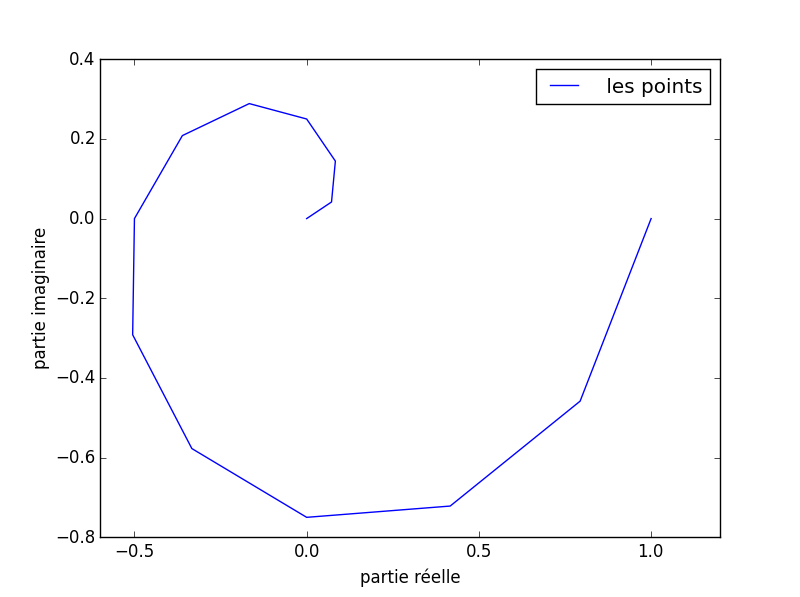
\includegraphics[width=7cm]{programmes/Exercice_2015_01/Exercice_2015_01_Chabert}

\textit{D'après Thibaut Decombe, PT$\star$ 2016 -- 2017.}
\begin{corrige}
$\quad$
\begin{python}
## 1 ##
zo=2 + 1j
def zn1(zn):
    return((zn+abs(zn))/2)

#print(zn1(zo))
z=zo
for i in range(12):
    z=zn1(z)
    
#print(z)  2.1568104230797602+0.000244140625j)
    
## 2 ##
    
def les_zn(zo,n):
    L=[zo]
    z=zo
    for i in range(n):
        L.append(zn1(z))
        z=zn1(z)
    return(L)
#print(les_zn(2+1j,2))

# [(2+1j), (2.118033988749895+0.5j), (2.1471424441163585+0.25j)]
\end{python}
\end{corrige}


\subsection*{Exercice 2}
\textit{D'après Léo Chabert, PT$\star$ 2016 -- 2017.}

\begin{corrige}
$\quad$
\begin{python}
# On suppose a<b
## Q1
def disjoint(i1,i2):
    """ retourne True si les segment sont disjoints, false sinon """
    return(i1[1]<i2[0] or i2[1]<i1[0])

#print(disjoint([0,1],[-1,0.5]))
#False

## Q2
def fusion(i1,i2):
    """ fusionne les deux segments """
    return([min(i1[0],i2[0]),max(i1[1],i2[1])])

#print(fusion([-1,2],[0,0.5])) [-1, 2]
#print(fusion([-1,2],[0,5])) [-1, 5]


## Q3

#L = [[0,3],[6,7],[2,5]]
#non bien fondée
L = [[0,1],[2,3],[4,5]]
#bien fondée

def verif(L):
    """ vérifie si une liste est bien fondée """

    if len(L) == 1 :
        return(True)
    elif disjoint(L[0],L[1]) and L[0][1]<L[1][0] :
        return(True and (verif(L[1:])))
    else :
        return(False)
    
#print(verif(L))
#True
\end{python}
\end{corrige}

\subsection*{Exercice 3}
\textit{D'après Léo Chabert, PT$\star$ 2016 -- 2017.}

\begin{corrige}
$\quad$
\begin{python}


## Q1

def est_cube(n) :
    """ vérifie qu'un nombre est un cube """
    return(int(n**(1/3))**3 == n )

#print(est_cube(8))
#print(est_cube(27))
#print(est_cube(12))

#True
#True
#False

Lcube = []

for i in range(251):
    if est_cube(i):
        Lcube.append(i)

# print(Lcube)
# [0, 1, 8, 27, 125]

        
## Q2

def S2cube(n) :
    """ vérifie qu'un nombre est la somme de deux cubes """
    
    res = False
    i = 0
    
    while i <= (n-1) and not(res) :
        if est_cube(n-i) and est_cube(i) :
            res = True
        i+=1
        
    return(res)

#print(S2cube(35))
#print(S2cube(30))

#True
#False



# Entier inférieur à 250 somme de 2 cubes :

##L2cube = []
##
##for i in range(251):
##    if S2cube(i):
##        L2cube.append(i)

#print(L2cube)
#[1, 2, 8, 9, 16, 27, 28, 35, 54, 125, 126, 133, 152, 250]


## Q3

def S4cube(n) :
    """ vérifie qu'un nombre est la somme de 4 cubes """
    
    res = False
    i = 0
    
    while i <= (n-1) and not(res) :
        if S2cube(n-i) and S2cube(i) :
            res = True
        i+=1
        
    return(res)

##
##L4cube = []
##
##for i in range(251):
##    if S4cube(i):
##        L4cube.append(i)

#print(L4cube)

""" [2, 3, 4, 9, 10, 11, 16, 17, 18, 24, 25, 28, 29, 30, 32, 35, 36, 37, 43, 44, 51, 
      54, 55, 56, 62, 63, 70, 81, 82, 89, 108, 126, 127, 128, 133, 134, 135, 141, 
       142, 149, 152, 153, 154, 160, 161, 168, 179, 180, 187, 206, 250]
"""

## Q4
def S8cube(n) :
    """ vérifie qu'un nombre est la somme de 8 cubes """
    
    res = False
    i = 0
    
    while i <= (n-1) and not(res) :
        if S4cube(n-i) and S4cube(i) :
            res = True
        i+=1
        
    return(res)


##L8cube = []
##
##for i in range(251):
##    if S8cube(i):
##        L8cube.append(i)
##    print(i)
##
##print(L8cube)
##
###[4, 5, 6, 7, 8, 11, 12, 13, 14, 15, 18, 19, 20, 21, 22, 25, 26, 27, 28, 29, 30, 31, 32, 33, 34, 35, 36, 37, 38, 39, 40, 41, 42, 43, 44, 45, 46, 47, 48, 49, 50, 51, 52, 53, 54, 55, 56, 57, 58, 59, 60, 61, 62, 63, 64, 65, 66, 67, 68, 69, 70, 71, 72, 73, 74, 75, 76, 78, 79, 80, 81, 82, 83, 84, 85, 86, 87, 88, 89, 90, 91, 92, 93, 94, 95, 97, 98, 99, 100, 102, 105, 106, 107, 108, 109, 110, 111, 112, 113, 114, 116, 117, 118, 119, 121, 124, 125, 126, 128, 129, 130, 131, 132, 133, 135, 136, 137, 138, 139, 140, 142, 143, 144, 145, 146, 149, 150, 151, 152, 153, 154, 155, 156, 157, 158, 159, 160, 161, 162, 163, 164, 165, 166, 167, 168, 169, 170, 171, 172, 173, 174, 176, 177, 178, 179, 180, 181, 182, 183, 184, 185, 186, 187, 188, 189, 190, 191, 192, 193, 195, 196, 197, 198, 200, 203, 204, 205, 206, 207, 208, 209, 210, 211, 212, 214, 215, 216, 217, 219, 222, 223, 224, 230, 231, 233, 234, 235, 236, 238, 241, 242, 243, 249, 250]

\end{python}
\end{corrige}

\end{document}

\textit{D'après Léo Chabert, PT$\star$ 2016 -- 2017.}
\textit{D'après Thibaut Decombe, PT$\star$ 2016 -- 2017.}

%\columnbreak
%\addcontentsline{toc}{subsection}{Exercice 4}
\subsection*{Exercice 8}

\begin{corrige}
$\quad$
\begin{python}

\end{python}
\end{corrige}




